\documentclass[10pt,a4paper]{article}
\usepackage[justification=centering]{caption}
\usepackage[pdfpagelabels,bookmarks,hyperindex,hyperfigures, hidelinks]{hyperref}
\usepackage[spanish]{babel}
\usepackage[toc, page]{appendix}
\usepackage[utf8]{inputenc}
\usepackage[version=4]{mhchem}
\usepackage{alltt}
\usepackage{amsmath}
\usepackage{circuitikz}
\usepackage{csquotes}
\usepackage{epstopdf}
\usepackage{fancyhdr}
\usepackage{gensymb}
\usepackage{lastpage}
\usepackage{multirow}
\usepackage{parskip}
\usepackage{pdfpages}
\usepackage{placeins}
\usepackage{subcaption}
\usepackage{tabularx}
\usepackage{textcomp}
\usepackage{tikz}
\usepackage{titlesec}
\usepackage{upgreek}
\usepackage{xfrac}

\usetikzlibrary{arrows, decorations.markings, positioning}

% Print a DRAFT water mark on the document
% Comment to remove for final version
%\usepackage{draftwatermark}
%\SetWatermarkText{ DRAFT }
%\SetWatermarkScale{5}

\setlength{\parskip}{0.6em}

% Set the indentation length 
\setlength{\parindent}{0em}

% Bibliography settings
\usepackage[backend=biber,style=ieee]{biblatex}
%\setbeamertemplate{bibliography item}{\insertbiblabel}
\addbibresource{major_paper.bib}

% Glossary entries
\usepackage[acronym, nomain]{glossaries}
\makenoidxglossaries

\newacronym{ARLB}{ARLB}{Aqueous rechargeable lithium batteries}
\newacronym{BMS}{BMS}{Battery Management System}
\newacronym{CAN}{CAN}{Controller Area Network}
\newacronym{CC}{CC}{Constant Current}
\newacronym{CV}{CV}{Constant Voltage}
\newacronym{DB}{DB}{Diagrama de Bloques}
\newacronym{DOD}{DOD}{Depth of Discharge}
\newacronym{EC}{EC}{Eficiencia Culombica}
\newacronym{EIS}{EIS}{Electrochemical Impedance}
\newacronym{FIR}{FIR}{Finite Impulse Response}
\newacronym{FPGA}{FPGA}{Field Programmable Gate Arrays}
\newacronym{HPPC}{HPPC}{Hybrid Pulse Power Characterization}
\newacronym{IISB}{IISB}{Institute for Integrated Systems and Device Technology}
\newacronym{Ion-Li}{Ion-Li}{Batería de Ion Litio}
\newacronym{KF}{KF}{Kalman Filter}
\newacronym{Li-Po}{Li-Po}{Batería de Polímero de Litio}
\newacronym{MCU}{MCU}{Microcontroller Unit}
\newacronym{MLE}{MLE}{Maximum Likelihood Estimation}
\newacronym{MSE}{MSE}{Mean Squared Error}
\newacronym{OCV}{OCV}{Open Circuit Voltage}
\newacronym{SOA}{SOA}{Secure Operation Area}
\newacronym{SOC}{SoC}{State Of Charge}
\newacronym{SOH}{SoH}{State Of Health}
\newacronym{TCR}{TCR}{Temperature Coefficient of Resistance}
\newacronym{UPS}{UPS}{Uninterruptible Power Supply}
\newacronym{VE}{VE}{vehículo eléctrico}
\newacronym{VVEE}{VVEE}{vehículos eléctricos}
\newacronym{hri}{HRI}{human-robot interactions}
\newacronym{lstm}{LSTM}{Long Short-Term Memory}
\newacronym{rnn}{RNN}{Recurrent Neural Network}

\tikzstyle{vecArrow} = [thick, decoration={markings,mark=at position
	1 with {\arrow[semithick]{open triangle 60}}},
double distance=1.4pt, shorten >= 5.5pt,
preaction = {decorate},
postaction = {draw,line width=1.4pt, white,shorten >= 4.5pt}]
\tikzstyle{innerWhite} = [semithick, white,line width=1.4pt, shorten >= 4.5pt]
\graphicspath{{assets/}} 
\newcommand\reaction[1]{\begin{equation}\ce{#1}\end{equation}} 

\titleclass{\subsubsubsection}{straight}[\subsection]

\newcounter{subsubsubsection}[subsubsection]
\renewcommand\thesubsubsubsection{\thesubsubsection.\arabic{subsubsubsection}}
\renewcommand\theparagraph{\thesubsubsubsection.\arabic{paragraph}} % optional; useful if paragraphs are to be numbered

\titleformat{\subsubsubsection}
  {\normalfont\normalsize\bfseries}{\thesubsubsubsection}{1em}{}
\titlespacing*{\subsubsubsection}
{0pt}{3.25ex plus 1ex minus .2ex}{1.5ex plus .2ex}

\makeatletter
\renewcommand\paragraph{\@startsection{paragraph}{5}{\z@}%
  {3.25ex \@plus1ex \@minus.2ex}%
  {-1em}%
  {\normalfont\normalsize\bfseries}}
\renewcommand\subparagraph{\@startsection{subparagraph}{6}{\parindent}%
  {3.25ex \@plus1ex \@minus .2ex}%
  {-1em}%
  {\normalfont\normalsize\bfseries}}
\def\toclevel@subsubsubsection{4}
\def\toclevel@paragraph{5}
\def\toclevel@paragraph{6}
\def\l@subsubsubsection{\@dottedtocline{4}{7em}{4em}}
\def\l@paragraph{\@dottedtocline{5}{10em}{5em}}
\def\l@subparagraph{\@dottedtocline{6}{14em}{6em}}
\makeatother

\setcounter{secnumdepth}{4}
\setcounter{tocdepth}{4}

\setcounter{MaxMatrixCols}{20}

\setlength{\headheight}{52pt}
\pagestyle{fancy}
\fancyheadoffset{0.5cm}
\fancyhead{}
\fancyhead[L]{
\includegraphics[scale=0.125]{FCEIA-logo.png}}
\fancyhead[C]{Universidad Nacional de Rosario\\
Facultad de Ciencias Exactas,Ingeniería y Agrimensura\\
Escuela de Ingeniería Electrónica}
\fancyhead[R]{
\includegraphics[scale=0.06]{LOGO-UNR-NEGRO.png}}

\renewcommand{\figurename}{Fig.}

\renewcommand\footrule{\begin{minipage}{0.95\textwidth}
    \hrule width \hsize   
\end{minipage}\par}

\setlength{\footskip}{30pt}
\fancyfoot[L]{\textit{Proyecto Final - F. Ceccarelli, M. Moya, L. Santos}}
\fancyfoot[C]{}
\fancyfoot[R]{\textit{Página \thepage{} de \pageref{LastPage}}}

\DeclareGraphicsExtensions{.bmp, .png, .jpg}

\renewcommand*\contentsname{Índice}

\topmargin = -1.5cm
\leftmargin = -1cm
\oddsidemargin = 0cm
\textheight = 24cm
\textwidth = 17cm

\begin{document}

\begin{titlepage}
    \begin{center}
	\begin{minipage}{.45\textwidth}
	    \flushleft
	    
\includegraphics[scale=0.25]{FCEIA-logo.png}
	\end{minipage}%
	\hspace{20mm}
	\begin{minipage}{.3\textwidth}
	    \flushleft
	    
\includegraphics[scale=0.1]{LOGO-UNR-NEGRO.png}
	\end{minipage}

	\vspace{15mm}

	\large{ \textbf{Universidad Nacional de Rosario}} \\[5mm]
	\textbf{Facultad de Ciencias Exactas, Ingeniería y Agrimensura} \\[5mm]
	Escuela de Ingeniería Electrónica \\[20mm]
	\Large {\textbf{Área de Gestión de Proyectos}}\\[1.5mm]
	\small {Ingeniería Electrónica} \\[20mm]
	\Large {\textbf{Proyecto Final}} \\[5mm]
	\Large{ \textbf{Estudio e Implementación de un Sistema de Administración de
	Baterías de Li-Ion de baja y mediana potencia}} \\[15mm]

    \end{center}

    \begin{minipage}[t]{0.6\textwidth}
	{\large\textbf{Autores:}}
	\begin{itemize}
	    \item [] Federico Ceccarelli (C-6241/3)
	    \item [] Martin Moya (M-6132/8)
	    \item [] Lucio Santos (S-4966/2)
	\end{itemize}
	\vspace{10pt}
	{\large\textbf{Directora:}}

	\begin{itemize}
	    \item [] Dra. Monica Romero
	\end{itemize}
	\vspace{10pt}
	{\large\textbf{Asesor:}}
	\begin{itemize}
	    \item [] Ing. Edgardo Arnejo
	\end{itemize}
    \end{minipage}

    \begin{minipage}[t]{0.35\textwidth}
	\flushleft
	\Large\textbf{Firma:}
    \end{minipage}

\end{titlepage}

\newpage

\begin{abstract}
    \noindent En el presente trabajo se detalla el proceso de desarrollo e
    investigaci\'on de un administrador de baterias o, tambien conocido como,
    \acrshort{BMS} (del ingles \emph{\acrlong{BMS}}) compatible con un pack
    de bater\'ias de iones de litio, capaz de estimar el estado de carga 
    utilizando filtros cuadr\'aticos, balancear, proteger, cargar y 
    comunicar, a trav\'es del protocolo \acrshort{CAN}, todas 
    las variables del mismo. El dispositivo es orientado a veh\'iculos 
    el\'ectricos de baja y mediana potencia, como por ejemplo, 
    bicicletas/monopatines hasta triciclos de transporte con carga
    y busca resolver mucha de las problem\'aticas intr\'insecas de 
    la tecnolog\'ia litio-ion, como por ejemplo, su volatilidad ante 
    operaciones fuera del \'area segura de operaci\'on, 
    como tambi\'en la falta de proyectos abiertos de esta \'indole en el mercado. 
    A pesar de estar caracterizado para veh\'iculos el\'ectricos, el mismo 
    puede ser aplicado a almacenadores de energ\'ia, tales como los paneles 
    solares, incluso hasta sistemas de alimentaci\'on ininterrumpida, o 
    \acrshort{UPS} (del ingles, \emph{\acrlong{UPS}}).
\end{abstract}

\newpage
% Print table of contents
\tableofcontents

\newpage

\section{Introducción}

\noindent A partir de la relevancia que ha comenzado a tomar el 
calentamiento global en las últimas décadas y el inquietante impacto que 
el mismo tiene sobre la calidad de vida de las personas, se han intentado 
buscar distintas soluciones para apaciguar las principales causas que 
generan un deterioro del medio ambiente, entre ellas, se encuentra el 
desarrollo de nuevas fuentes de energía renovables y su aprovechamiento.

\noindent El \acrfull{VE} \emph{(fig. \ref{EV})} es considerado 
una de las transiciones tecnológicas más importantes de los últimos años 
debido a que no emiten dióxido de carbono ($\mathrm{CO_2}$) al medio 
ambiente y no utilizan combustibles fósiles para su funcionamiento, esto 
los convierte en uno de los avances tecnológicos más atractivos de los 
últimos tiempos teniendo en cuenta el avance del calentamiento global y el 
crecimiento del valor del petróleo.

\begin{figure}[h!]
    \begin{center}
	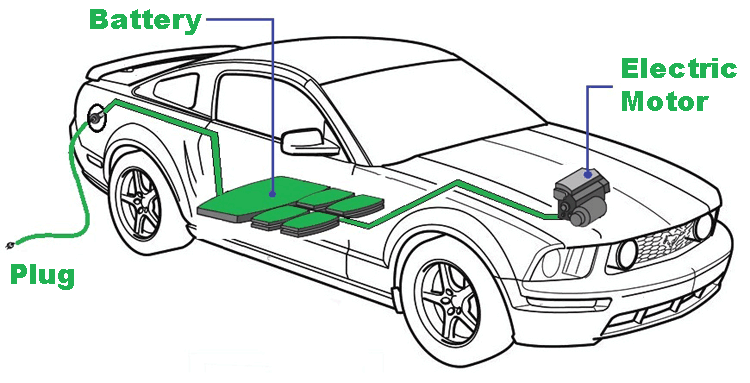
\includegraphics[width=0.7\textwidth]{EV.png}
	\caption{Esquem\'atico de un veh\'iculo electrico}
	\label{EV}
    \end{center}
\end{figure}

\noindent Siendo las baterías eléctricas la única fuente de energía en los 
\acrfull{VVEE}, éstas tienen un gran impacto en la performance de los mismos 
determinando la autonomía del vehículo. En base a este criterio, las 
baterías de iones de litio (\emph{Li-Ion}) resultan las más adecuadas para 
esta aplicación debido a su alta densidad energética, es decir, que éste 
tipo de baterías tienen una gran capacidad para su reducido volumen a 
comparación de otras tecnologías. Para poder ser utilizados en
\acrshort{VVEE}, las baterías de Li-Ion son conectadas en forma de arreglos 
o packs de baterías en serie que permiten obtener mayores valores de tensión
y, otras, en paralelo para aumentar la capacidad del pack.

\subsection{Motivaci\'on del proyecto}

\noindent Una de las grandes problem\'aticas de las bater\'ias de Litio-ion 
reside en que se debe tener en cuenta ciertas precauciones a la hora de
implementarlas, debido a que las mismas son propensas a fallar al ser 
sobrecargadas, completamente descargadas u operadas fuera del
rango seguro de temperatura, tensi\'on o corriente, adem\'as, en un pack de 
bater\'ias conectadas en serie, se pueden manifestar pequeñas diferencias de 
capacidades a traves de todas las celdas, causado por tolerancias de
producci\'on o diferentes condiciones de operaci\'on, que tienden
a incrementar con cada ciclo de carga. Por \'ultimo, las bater\'ias
sufren un proceso de \emph{auto-descarga} (t\'ipicamente entre un
2-10\% dependiendo de la temperatura y el estado de carga de la misma). 
Si la distribuci\'on de temperatura a lo largo del pack es
heterog\'enea, las celdas con mayor temperatura tienden a una mayor
p\'erdida de capacidad provocando un desbalanceo de carga.
Esto trae varias consecuencias, entre ellas, se encuentran:

\begin{itemize}
    \item \textbf{Seguridad:} Si el voltaje máximo de carga es excedido por 
	unos cientos de milivoltios, puede provocar un embalamiento térmico, 
	derritiendo el pack de baterias y, por lo tanto, el dispositivo que 
	alimenta. En el peor de los casos puede explotar poniendo en riesgo el 
	bienestar del usuario.
    \item \textbf{Salud de la batería:} La degradación de la batería es 
	extremadamente sensible a la operación de la misma fuera de la zona 
	indicada. Si la temperatura de operación o la tensión máxima de carga 
	es excedida esto provoca una aceleración en la degradación de su vida 
	útil.
    \item \textbf{Autonomía:} Consideremos que el circuito de protección 
	detecta que una de las baterías se encuentra descargada a niveles 
	cercanos de operación insegura. En este caso, la protección frena la 
	descarga del pack por una sola celda y el resto se encuentran con 
	voltajes más altos y, por lo tanto, con un remanente de energía para 
	entregar a la carga desaprovechando la capacidad del pack entero.
\end{itemize}

\noindent Lo que conllevan a la implementación de un sistema de administración 
de baterías (\emph{\acrshort{BMS}} por sus siglas en inglés \acrlong{BMS}). En
definitiva, un \acrshort{BMS} es un dispositivo encargado de controlar las
funciones vitales de las baterías para que operen de forma correcta y segura, 
con el objetivo de otorgar seguridad al usuario y prolongar la autonomía del 
vehículo. Las funciones más relevantes que llevan a cabo son:

\begin{itemize}
    \item Protección del pack para su operación en la región segura tanto 
	en tensión, corriente como también en temperatura.
    \item Ecualización de las celdas individuales del pack, es decir,
	controlar que la carga entre celdas sea uniforme
    \item Estimación del estado de carga del pack de batería 
        (\emph{\acrshort{SOC}} por sus siglas en ingl\'es \acrlong{SOC}).
    \item Estimación del estado de salud del pack de batería 
        (\emph{\acrshort{SOH}} por sus siglas en ingl\'es \acrlong{SOH}).
    \item Informar a la computadora central del vehículo los distintos 
	parámetros del pack de baterías.
\end{itemize}

\noindent Ademas de las problem\'aticas mencionadas anteriormente, en el mercado
actual se venden una gran variedad de \acrshort{BMS} con escaza documentaci\'on
sobre el mismo, dificultando su implementaci\'on con otros dispositivos, tales 
como computadoras centrales de veh\'iculos el\'ectricos hasta \acrshort{UPS}.

\noindent Por su contraparte, existen solamente dos proyectos de 
c\'odigo/hardware abiertos relacionados al desarrollo de \acrshort{BMS}, 
detallados a continuaci\'on.

\subsubsection{foxBMS}

\emph{foxBMS} es un proyecto desarrollado por el Instituto de Sistemas
Integrados y Tecnolog\'ias de Dispositivos de la sociedad \emph{Fraunhofer} o
tambien llamado Fraunhofer IISB (del ingles \emph{\acrlong{IISB}}), una
organización de investigación alemana que comprende 72 institutos esparcidos por
todo el territorio alem\'an.

\noindent El desarrollo de este proyecto es el resultado de 15 años de
investigaci\'on en el \'area de energ\'ias renovables y es diseñado para 
administrar innovadores prototipos de sistemas de bater\'ias basados en la 
tecnolog\'ia iones de litio, desde pocas celdas conectadas en serie hasta 
centenares de kWh y kW, especialmente para sistemas que requieren altos niveles 
de fiabilidad.

\noindent El proyecto no tiene intenciones de ser usado de forma comercial en
productos ya que no cumple con estandards espec\'ificos y requieren determinados
certificados para ser vendidos en el mercado. Solamente cumple con el 
prop\'osito de ser una plataforma de ensayo y desarollo que provee todas las 
funcionalidades del manejo de la complejidad y tamaño de los sistemas de 
almacenamiento mas avanzados al d\'ia de la fecha.

\noindent Si bien el mismo tiene extensa documentacion, originalmente fue
desarrollado para manejar packs de 12 a 18 celdas en serie, lo cual excede el
prop\'osito de la aplicaci\'on en cuestion por lo que no resulta viable para ser
implementado de forma directa. Tambien el hardware del proyecto es
extensivamente costoso y complejo, ya que implementa varios microcontroladores e
integrados dedicados hasta \acrshort{FPGA}s (del ingles, \emph{\acrlong{FPGA}}).

\subsubsection{openBMS}

A diferencia de \emph{foxBMS}, este proyecto fue desarrollado por ingenieros
independientes con el objetivo de diversificar los proyectos abiertos relativos
al tema en cuesti\'on.

\noindent El mismo busca desarrollar un \acrshort{BMS} capaz de manejar un
pack de bater\'ias de 4 a 96 celdas en serie, realizar el balanceo de las mismas 
y comunicar las variables del pack a traves del protocolo \acrshort{CAN}.

\noindent Si bien, se encuentran todos los archivos del proyecto a disposición
del publico, la documentaci\'on es muy escaza para ser implementado
f\'acilmente para un proyecto relacionado.

\noindent En definitiva, las motivaciones para llevar a cabo el presen trabajo
se basan en la complejidad en el manejo de grandes packs de
bater\'ias basadas en celdas de litio-ion y la falta de proyectos abiertos
disponibles relacionados al tema.

\noindent Finalmente, el informe se encuentra dividido en 6 secciones, en
la Seccion \ref{descripcion} se realiza una descripci\'on en alto nivel del
proyecto, detallando los objetivos generales, las especificaciones y
requerimientos del trabajo, a continuaci\'on, se encuentra el fundamento 
te\'orico (Secci\'on \ref{teoria}), donde se detalla el funcionamiento de una 
celda de litio-ion, los fundamentos b\'asicos de modelados de celdas y 
algoritmos de estimaci\'on de carga, como tambi\'en aquellos relacionados a la 
equalizaci\'on de celdas, adem\'as, se presenta el desarrollo matem\'atico de 
mucho de los m\'etodos como tambi\'en una comparativa, por ultimo se presentan 
las secciones \ref{desarrollo} y \ref{ensayos} donde se describe el desarrollo 
de la bater\'ia en si, en conjunto con su modelo y algoritmos como tambi\'en su 
final implementaci\'on en un sistema embebido con los ensayos realizados para 
validar el funcionamiento del sistema. Finalmente, en la secci\'on 
\ref{conclusiones} se describen las conclusiones y futuros proyectos a continuar 
sobre el eje de estudio.

\section{Descripci\'on}\label{descripcion}

\subsection{Objetivos Generales}

Como solución a los problemas planteados, se propone desarrollar un 
\acrshort{BMS} que cumpla con los siguientes requisitos:

\begin{itemize}
    \item Proteger el pack de baterías evitando que el mismo salga de su 
	zona de operación segura, tanto en tensión, corriente como en 
	temperatura, evaluando los umbrales correspondientes para las celdas de 
    Litio-Ion.
    \item Estimar el estado de carga en tiempo real.
    \item Balancear la carga entre celdas, priorizando el menor costo 
	energético posible del sistema y la mayor autonomía final del pack.
    \item Comunicar los parámetros fundamentales del pack a una computadora 
	central a través de algún protocolo estandarizado.
\end{itemize}

\noindent Para lograr estos objetivos, se plantea un estudio pormenorizado 
del estado del arte de la temática en cuestión procurando seleccionar las 
prácticas y metodologías más adecuadas para la solución del problema 
planteado, a partir de un estudio teórico. Finalmente se validará la 
solución elegida a partir de la implementación y ensayo de la solución 
desarrollada.

\subsection{Especificaciones}

\noindent El sistema a implementar debe ser capaz de poder administrar un 
pack de bater\'ias de 6 m\'odulos conectados en serie, donde cada modulo est\'a 
compuesto por 3 celdas en paralelo encargado de: 

\begin{itemize}
    \item Sensar la tensión de las celdas individuales del pack y de la 
	corriente que circula desde y hacia el pack as\'i como tambi\'en 
	la temperatura media.
    \item Realizar el balanceo de los m\'odulos que componen a la bater\'ia.
    \item Proteger el mismo, desconectando el pack de bater\'ias de la carga
	frente a operaciones fuera de la zona segura.
    \item Estimar el estado de carga y detectar las celdas que se encuentran
	en desbalance utilizando una unidad de cómputo como por ejemplo, un
	microcontrolador o \acrshort{MCU} (del ingl\'es \emph{\acrlong{MCU}}).
    \item Controlar el proceso de carga del pack de bater\'ias.
    \item Comunicar las variables del sistema a una computadora central a
	trav\'es de un protocolo especificado
\end{itemize}

\noindent La descripción anterior se puede visualizar en el \acrfull{DB} de la
Figura \ref{bms}. Como puede observarse, el microcontrolador es el encargado de
comunicarse y comandar los modulos de protecci\'on, ecualizaci\'on y carga de 
la bateria, como tambi\'en obtener variables de los mismos para poder estimar 
el \acrshort{SOC}, determinar el desbalanceo de una o m\'as celdas y tomar 
acci\'on al respecto, y por último, pero m\'as relevante, comandar las 
protecciones en caso de una falla y/o alerta de la batería. 
De forma simult\'anea, el mismo debe estar a cargo de comunicar las distintas 
variables del sistema a una computadora central.

\begin{figure}[h!]
    \begin{center}
	\begin{circuitikz}[european]
	    \draw (-4, -1) rectangle (-2, 1)[fill=blue!10!white];
	    \node at (-3, 0.2) {CPU};
	    \node at (-3, -0.2) {Central};
	    \draw [vecArrow] (-1.8, 0) to (-1, 0);
	    \draw [vecArrow] (-1.2, 0) to (-2, 0);

	    \draw (-1, -1) rectangle (1, 1)[fill=blue!10!white];
	    \node at (0, 0) {MCU};

	    \draw [blue,thin,dashed] (2.1, 2.5) rectangle (5.1, -2.5)[fill=blue!10!white];

	    \draw (2.2, 2.4) rectangle (5.0, 0.92)[fill=yellow!15!white];
	    \draw (2.2, 0.82) rectangle (5.0, -0.71)[fill=yellow!15!white];
	    \draw (2.2, -0.81) rectangle (5.0, -2.4)[fill=yellow!15!white];

	    \node at (3.6, 1.6) {Protección};           
	    \node at (3.6, -1.6) {Cargador};
	    \node at (3.6, 0) {Equalizaci\'on};
	    \draw [vecArrow] (1.2, 0) to (2.1, 0);
	    \draw [vecArrow] (1.5, 0) to (1, 0);

	    \draw (7, 2) -- (7, 2.2);
	    \draw (7, 2) to[battery1] (7, 1.6);
	    \draw (7, 1.4) -- (7, 1.6);
	    \draw (7, 1.4) to[battery1] (7, .9);            
	    \draw (7, .7) -- (7, .9);           
	    \draw (7, 0.7) to[battery1] (7, 0.2);           
	    \draw (7, 0.2) -- (7, -0.2);
	    \draw (7, -0.2) to[battery1] (7, -0.7);
	    \draw (7, -.7) -- (7, -.9);
	    \draw (7, -.9) to[battery1] (7, -1.4);
	    \draw (7, -1.4) -- (7, -1.6);
	    \draw (7, -1.6) to[battery1] (7, -2);
	    \draw (7, -2) -- (7, -2.2);

	    \draw (9, 2) -- (9, 2.2);
	    \draw (9, 2) to[battery1] (9, 1.6);
	    \draw (9, 1.4) -- (9, 1.6);
	    \draw (9, 1.4) to[battery1] (9, .9);            
	    \draw (9, .7) -- (9, .9);           
	    \draw (9, 0.7) to[battery1] (9, 0.2);           
	    \draw (9, 0.2) -- (9, -0.2);
	    \draw (9, -0.2) to[battery1] (9, -0.7);
	    \draw (9, -.7) -- (9, -.9);
	    \draw (9, -.9) to[battery1] (9, -1.4);
	    \draw (9, -1.4) -- (9, -1.6);
	    \draw (9, -1.6) to[battery1] (9, -2);
	    \draw (9, -2) -- (9, -2.2);

	    \draw (11, 2) -- (11, 2.2);
	    \draw (11, 2) to[battery1] (11, 1.6);
	    \draw (11, 1.4) -- (11, 1.6);
	    \draw (11, 1.4) to[battery1] (11, .9);          
	    \draw (11, .7) -- (11, .9);         
	    \draw (11, 0.7) to[battery1] (11, 0.2);     
	    \draw (11, 0.2) -- (11, -0.2);
	    \draw (11, -0.2) to[battery1] (11, -0.7);
	    \draw (11, -.7) -- (11, -.9);
	    \draw (11, -.9) to[battery1] (11, -1.4);
	    \draw (11, -1.4) -- (11, -1.6);
	    \draw (11, -1.6) to[battery1] (11, -2);
	    \draw (11, -2) -- (11, -2.2);

	    \draw (5.1, 0) to[short, -*] (7, 0);
	    \draw (7, 0) to[short, -*] (9, 0);
	    \draw (9, 0) to[short, -*] (11, 0);

	    \draw (7, 0.8) to[short, -*] (9, 0.8);
	    \draw (9, 0.8) to[short, -*] (11, 0.8);

	    \draw (7, 1.5) to[short, -*] (9, 1.5);
	    \draw (9, 1.5) to[short, -*] (11, 1.5);

	    \draw (7, 2.2) to[short, -*] (9, 2.2);
	    \draw (9, 2.2) to[short, -*] (11, 2.2);         

	    \draw (7, -0.8) to[short, -*] (9, -0.8);
	    \draw (9, -0.8) to[short, -*] (11, -0.8);

	    \draw (7, -1.5) to[short, -*] (9, -1.5);
	    \draw (9, -1.5) to[short, -*] (11, -1.5);

	    \draw (7, -2.2) to[short, -*] (9, -2.2);
	    \draw (9, -2.2) to[short, -*] (11, -2.2);           

	    \draw (5.1, 0.2) -- (6.2, 0.2) |- (7, 0.8) node at (7, .8){$\bullet$};
	    \draw (5.1, 0.4) -- (6, 0.4) |- (7, 1.5) node at (7, 1.5){$\bullet$};
	    \draw (5.1, 0.6) -- (5.8, 0.6) |- (7, 2.2) node at (7, 2.2){$\bullet$};

	    \draw (5.1, -0.2) -- (6.2, -0.2) |- (7, -0.8) node at (7, -.8){$\bullet$};
	    \draw (5.1, -0.4) -- (6, -0.4) |- (7, -1.5) node at (7, -1.5){$\bullet$};
	    \draw (5.1, -0.6) -- (5.8, -0.6) |- (7, -2.2) node at (7, -2.2){$\bullet$};

	    \draw [dashed] (-1.2, 2.6) rectangle (5.2, -2.6);
	    \draw node at (-.8, 2.8){BMS};

	    \draw [dashed] (6.5, 2.4) rectangle (11.5, -2.4);

	    \draw node at (8.2, 2.6) {Pack de Baterías 6s3p};

	    \draw (13, 1) to[R=$Z$] (13, -1);

	    \draw (11, 2.2) -- (12, 2.2)
	    |- (12, 1.5) -- (13, 1.5) |- (13,1) node at (12, 1.5){$\bullet$};

	    \draw (11, -2.2) -- (12, -2.2)
	    |- (12, -1.5) -- (13,-1.5) |- (13,-1) node at (12, -1.5){$\bullet$};

	    \draw node at (12.8, 1){+};
	    \draw node at (12.8, -1){-};  
	\end{circuitikz}
    \end{center}
    \caption{Diagrama en Bloques del \acrshort{BMS} y el pack de baterías}
    \label{bms}
\end{figure}

\section{Aspectos Te\'oricos}\label{teoria}

\subsection{Batería de Litio-Ion}

La energía eléctrica ha empoderado a la sociedad desde su descubrimiento y,
gracias a sus avances tecnológicos, el acceso a la misma se ha convertido mas
facil y mas eficiente, aun así con la ausencia de conexiones eléctricas en la
cercania. Sumado a eso, tambien nos dirigimos a una sociedad que aprovecha de la
movilidad a medida que los dispositivos dependen menos de una conexi\'on 
el\'ectrica local.

\noindent En gran parte, estos desarrollos son posibles gracias al
descubrimiento del litio-ion y su aplicacion en baterías. Este tipo de batería
ha revolucionado la tecnolog\'ia en almacenamiento de energ\'ia y ha logrado
impulsar la revoluci\'on digital empoderando los dispositivos moviles, 
a trav\'es de su gran capacidad y densidad energ\'etica.

\subsubsection{Principios b\'asicos}

El principio básico de funcionamiento de una batería, en su configuraci\'on
b\'asica, consiste en una celda compuesta por dos electrodos 
\emph{(fig. \ref{batt_wk_ppl})}, cada una conectada a un circuito el\'ectrico, 
separado por un electrolito que es capaz de acomodar cargas dentro de sí. 
Frecuentemente, los electrodos son f\'isicamente separados por una barrera que 
previene que estén en contacto físico entre ellos, evitando así un corto 
circuito en la bateria. En descarga, cuando la bater\'ia entrega corriente al 
circuito, toma lugar un proceso de oxidación en el electrodo negativo (\'anodo), 
resultando en un movimiento de electrones a trav\'es del circuito. Por el otro 
lado, en el electrodo positivo (c\'atodo), ocurre un proceso de reducción, 
reabastecido por los electrones del circuito. El voltaje de la celda depende 
fuertemente de la diferencia de potencial entre los electrodos, y del proceso 
espont\'aneo en su totalidad. Para baterías recargables el proceso puede ser 
reversible aplicando electricidad externa produciendo un proceso complementario 
de \emph{redox} (reducci\'on-oxidac\'on) en los electrodos. Este proceso es 
dependiente de la energ\'ia y es no espont\'aneo, es decir, que sucederá s\'i y 
solo s\'i un agente externo participa en el proceso.

\noindent En base a este principio de funcionamiento, surgen una gran variedad
de tecnologías, partiendo de la pila voltaica, hecha de dos discos de metales
distintos, uno de zinc y otro de cobre o plata, separados por un dieléctrico
(como cartón o cuero) sumergido en una solución electrolítica. Durante la
operación, el disco de zinc actua como ánodo, liberando electrones al circuito y
produciendo iones de metal (proceso de oxidación), mientras que la reacción en
el electrodo opuesto depende de las condiciones de trabajo. En presencia del
aire, el metal de cobre es parcialmente oxidado a CuO, y la reducción de CuO a
Cu se da en el electrodo. En la ausencia de aire, los protones en el electrolito
son reducidos a hidrógeno en la superficie del cobre. El voltaje de la celda es
de aproximadamente 0.8-1.1V, dependiendo de la exposición al aire. 
Esencialmente, la pila voltaica es una batería no recargable.

\begin{figure}[h!]
    \begin{center}
	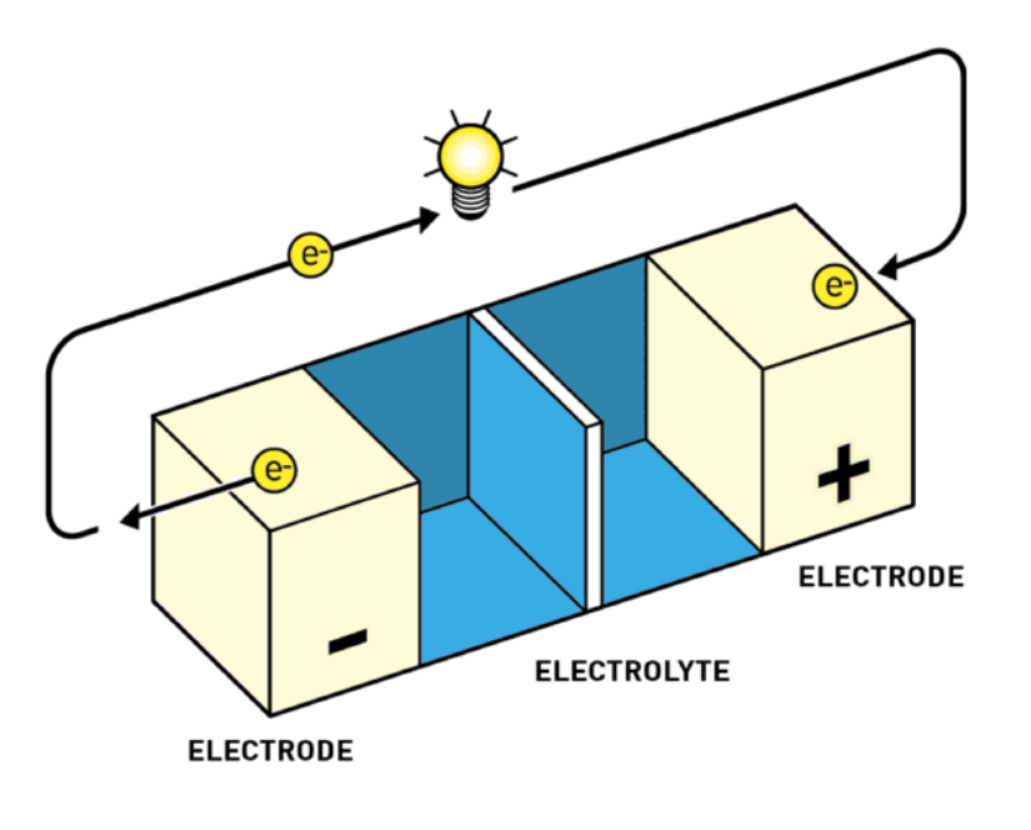
\includegraphics[width=0.4\textwidth]{batt_func_ppr.png}
    \end{center}
    \caption{Diagrama del principio básico de funcionamiento de una bater\'ia 
        en el proceso de descarga.}
    \label{batt_wk_ppl}
\end{figure}

\noindent Despu\'es surgieron las baterías de plomo-ácido, que su principio
de operaci\'on es similar a las baterías voltaicas expuestas al aire, pero con
la posibilidad de ser recargadas. Esta tecnología se basa en dos electrodos de
plomo, donde uno se encuentra parcialmente oxidado, en este caso es  oxido de 
plomo ($\mathrm{PbO_2}$), separado por \'acido sulf\'urico que contiene un 
electrolito. Durante el proceso de descarga, ocurre un proceso de oxidaci\'on 
en el electrodo de plomo (\'anodo), produciendo electrones, protones y sulfato 
de plomo ($\mathrm{PbSO_4}$), mientras que el \'oxido de plomo es reducido a
$\mathrm{PbSO_4}$ en el cátodo. En este caso, el potencial de una celda es de
alrededor 2V.

\noindent Otro logro en el desarrollo de baterías, ocurrió en el 1899 cuando se
desarrolló la primer batería de niquel-hierro (Ni-Fe) y niquel-cadmio (Ni-Cd) o
tambien conocidas como baterias alcalinas, que fueron predecedoras del híbrido
niquel-metal (Ni-MH) que fue comercializada en 1898.

\noindent Las baterías anteriores son basadas en soluciones acuosas, y la
densidad energetica de las mismas no es alta, espec\'ificamente son menores a 
los 100Wh/kg. Para incrementar la densidad energética de estas baterías, es
necesario encontrar una estabilidad electroquímica del agua ya que juega un rol
muy importante en ello. Además, cuando \'ambos electrodos utilizando el alto
potencial del plomo, el voltaje de salida solo puede alcanzar un máximo de 2.2V.
Como resultado de los avances tecnol\'ogicos dentro del mercado de consumo
electr\'onico y, como consecuencia, con la necesidad de incrementar la densidad 
energética de una celda, se impuls\'o la b\'usqueda de nuevas tecnolog\'ias que
permitan obtener una mayor capacidad en las bater\'ias con un tamaño reducido, 
se descubrio el potencial del metal de litio y su aplicacicación en las 
celdas que llevan su nombre.

\subsubsection{Litio}

El litio es un metal descubierto en 1818 que tiene excelentes propiedades para
servir como material para el desarrollo de baterías. Es el metal m\'as liviano
con una densidad de 0.53$\mathrm{g/cm^3}$. Tambi\'en tiene un potencial de
reducci\'on muy bajo, que lo hace ideal para celdas de alta densidad y alto
voltaje. Sin embargo, es un metal reactivo que debe ser protegido, por ejemplo,
del agua y del aire, ya que el contacto con estos provoca que el mismo sea muy
complicado de controlar, imposibilitando su uso para la aplicación deseada. Esta
protección al medio no es trivial, y factores, tales como su caracter inerte,
punto de fusión, la estabilidad del \emph{redox}, solubilidad de iones de litios
y sales, velocidades de transferencia ion/electrón, viscosidad, entre otros,
deben ser considerados.

\noindent Las primeras baterías de litio alcanzaron el mercado en 1970 y la
comercialización de las mismas comenzó en Japón en el año 1991, cuando
\emph{Sony Corporation} presentó el primer modelo.

\noindent Las baterías de litio-ion son definidas en \cite{def_liion} como
almacenadores de energía que utilizan iones de Litio como portadores de carga.
En base a esta definición, el término \emph{batería de Litio-Ion} no se
corresponde con una sola composición química, como lo son las baterías de ácido
o niquel-cadmio, si no que expresa una familia de baterías que dependen de los
iones de litio pero que pueden ser conformadas por distintos materiales.

\noindent A diferencia de las baterías de ácido, hay dos razones principales por
las cuales las baterías de litio-ion han crecido en popularidad en tan poco
tiempo: su excelente rendimiento y la capacidad de adaptarse al creciente
mercado de la electrónica de consumo, como por ejemplo, videograbadoras,
celulares y computadoras. A partir de la primer década del siglo XXI, se
comenzaron a utilizar en vehículos eléctricos, como también en grandes sistemas
de almacenamiento de energía, capaces de alimentar barrios residenciales
enteros.

\noindent Desde el 2000 al presente, se desarrollaron varios tipos de 
bater\'ias basadas en el litio. Entre ellas se encuentran las bater\'ias de 
litio-sulfuro (Li-S) y litio-aire (Li-air), cuya densidad energética teórica 
ronda los 2600Wh/kg y 11400 Wh/kg, respectivamente. En 2012, se desarrolló una 
bateria de litio-ion recargable acuosa o \acrshort{ARLB} (del ingles
\emph{\acrlong{ARLB}}), que utiliza metal de litio recubierto como ánodo en una
solución de electrolitos mejorando ampliamente la densidad energética.

\subsubsection{Principio de funcionamiento}\label{battery_fun}

El principio de los procesos de carga y descarga en las baterías de litio-ion se
basan en utilizar óxido de litio-cobalto ($\mathrm{LiCoO_2}$) y grafito como
típicos materiales de electrodo. La Figura \ref{op_lithium-ion} ilustra el
princio de operación, y las reacciones de los electrodos se expresan en  las
Ecuaciones \ref{li_anode}, \ref{li_catode} y \ref{li_total}

\reaction{\text{Electrodo positivo: } LiCoO2 <=>[Carga][Descarga] Li_{1-x}CoO2 + xLi + xe^- \label{li_anode}}
\reaction{\text{Electrodo negativo: }6C + xLi^+ + xe^- <=>[Carga][Descarga] Li_{x}C6 \label{li_catode}}
\reaction{\text{Reaccion total: }6C + LiCoO2 <=>[Carga][Descarga] Li_{x}C6 + Li_{1-x}CoO2 \label{li_total}}

\noindent El \ce{LiCoO2} tiene una estructura reticular octa\'edrica con un
arreglo alternativo de capas de \ce{Li+} y \ce{Co^{3+}}. Durante el proceso de
carga, los iones de litio (en estado iónico) se desintercalan de la estructura
de capas del material del electrodo positivo, liberando electrones, al mismo
tiempo, el \ce{Co^{3+}} se oxida convirti\'endose en \ce{Co^{4+}}.  Por el otro
lado, durante el proceso de descarga, con la intercalación de \ce{Li+} dentro de
la ret\'icula, el \ce{Co^{4+}} es reducido a \ce{Co^{3+}}, ganando electrones,
adem\'as se obtienen electrones de la ret\'icula para convertirse en litio en 
estado atómico. Durante este proceso, el estado atómico del litio pierde 
electrones convirtiendose en iones de litio, este proceso se puede resumir en 
que el ánodo provee al electrodo positivo iones de litio. Dado que el litio se 
mueve entre el electrodo positivo y negativo hacia ambos lados a este tipo de 
baterías se las puede redefinir como una batería mecedora (del ingles,
\emph{rocking chair}).

\begin{figure}[h!]
    \begin{center}
	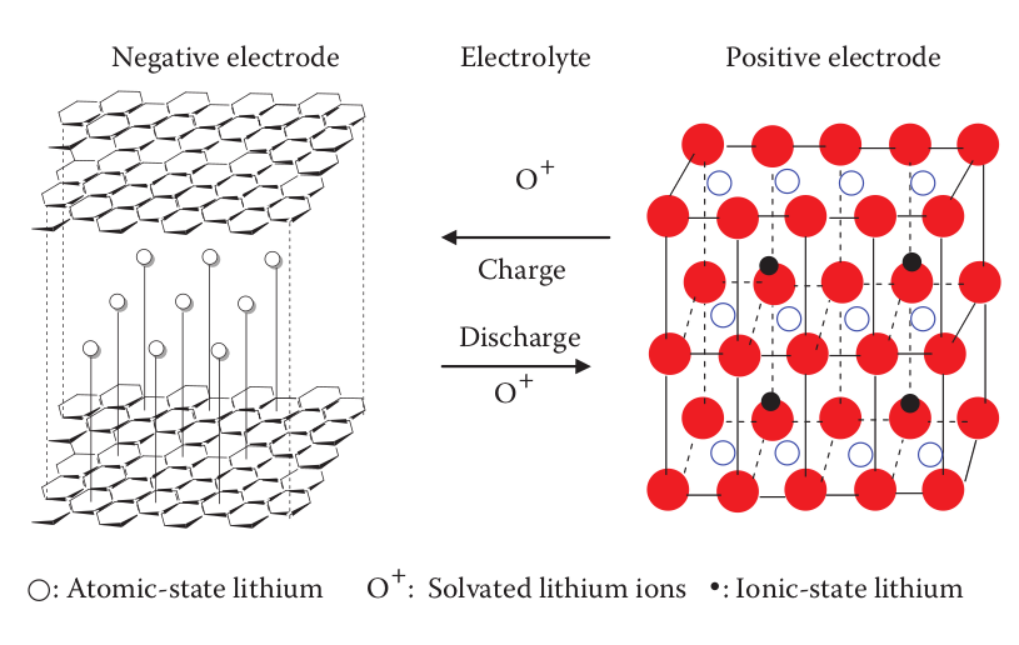
\includegraphics[width=0.7\textwidth]{prin_litio}
	\caption{Esquem\'atico del principio de operaci\'on de una bater\'ia de
	litio-ion.}
	\label{op_lithium-ion}
    \end{center}
\end{figure}

\noindent La mayoría de estas baterías usan materiales de carbón, tales como el
grafito y el carbón duro como ánodo. Otros utilizan óxidos de metales, como por
ejemplo, el titanato de litio ($\mathrm{Li_4Ti_5O_{12}}$) y el pentóxido de
niobio ($\mathrm{Nb_2O_5}$), debido a que pueden aceptar iones de litio cuando
son cargados, y liberarlos en el proceso de descarga, \'estas reacciones se
denominan como inserción y extracción respectivamente. Los potenciales de
reacción de estos materiales son mucho más bajos que los electrodos de hidrógeno
estándares, por lo tanto, el electrolito debería ser estable inclusive para
niveles de potencial tan bajos. Ésta es la razón por la cual, los electrolitos
orgánicos, que consisten de solventes orgánicos y sales de litio, son utilizados
en las baterías de Litio-ion en vez de electrolitos acuosos.

\noindent El material activo del cátodo debe contener Litio en su composición
química para proveer una fuente de iones de litio. Durante la primer etapa de
desarrollo de las celdas de litio, se utilizaba \'oxido de litio-cobalto.
También se estudió el uso de $\mathrm{LiNiO_2}$ como material activo para el 
cátodo pero fue inmediatamente descartado debido a su inestabilidad térmica. 
Sin embargo, se desarrollaron y utilizaron derivativos de esta composición, 
formulados como $\mathrm{LiM_xNi_{1-x}O_2}$  (M: elemento metálico tales como, 
el Co, Mn, Al, Mg).

\noindent Comparada con las baterías de litio-ion originales en los principios 
de 1990, el rendimiento de las mismas ha sido mejorado de forma significativa 
con el paso del tiempo. Los últimos desarrollos tienen ventajas dominantes sobre 
las baterías recargables tradicionales:

\begin{itemize}
    \item \textbf{Alta densidad energética:} La densidad energética por
	volumen y masa para una batería de litio modelo 18650 puede alcanzar
	los 500 Wh/$\mathrm{dm^3}$ y 230 Wh/kg, respectivamente, que adem\'as
	se encuentra en continuo aumento a medida que se investigan y
	desarrollan nuevas tecnologías.
    \item \textbf{Alto voltaje de salida (3.6V):} Esto es 3 veces 
        mayor a las baterías recargables de Ni-Cd o Ni-MH.
    \item \textbf{Alta potencia de salida:} Pueden alcanzar hasta 2kW/kg for
	un corto per\'iodo de tiempo.
    \item \textbf{Baja auto-descarga:} La descarga media de las celdas de
	litio son menores a un 3\% mensuales, que es la mitad que las celdas
	basadas en Ni-Cd y Ni-MH.
    \item \textbf{Bajo efecto de histéresis} A diferencia de las celdas de
	Ni-Cd y Ni-MH las celdas de litio tienen un efecto de histéresis
	despreciable con el paso de los ciclos de carga-descarga de la
	misma, resultando en un mejor ciclo de vida con respecto a los otros
	tipos de celdas.
    \item \textbf{Ciclos de carga-descarga rápidos:} Las baterías de
	litio-ion pueden ser cargadas con corrientes de hasta un 80\% de su
	capacidad. Es decir, si la batería tiene una capacidad de 3Ah, la
	misma se puede cargar a una corriente de 3A.
    \item \textbf{Alta eficiencia cul\'ombica:} La \acrlong{EC} o \acrshort{EC},
	es un par\'ametro que permite obtener que porcentaje del material
	activo se convierte en energia. Su medici\'on es importante porque 
	permite medir el desempeño de la bater\'ia con respecto a otras 
    tecnologias. En el caso de las celdas de Litio-ion, la \acrlong{EC}
	se mantiene casi en un 100\% inclusive despues del primer ciclo.
    \item \textbf{Gran rango de temperaturas}: Las bater\'ias de litio-ion
	pueden operar entre -25\degree C a +45\degree C. Las
	investigaciones actuales quieren extender ese rango desde -40\degree C a 
    +70\degree C con mejoras en el electrolito y los materiales de los 
    electrodos.

	Esto depende fuertemente del  alto voltaje, porque la energía específica es 
    el producto del voltaje de la celda y su capacidad específica, lo que hace 
    que las celdas de litio-ion se destaquen a comparación de otras tecnologías, 
	como por ejemplo, las celdas de Niquel-metal con un voltaje de 1.2V 
	pero con mayor capacidad tienen menor energía específica. 
    \item \textbf{Alta eficiencia energética:} Esto se debe a dos 
	factores principales, por un lado se debe a la alta eficiencia de 
	carga y descarga debido a que no hay pérdidas durante las reacciones 
	químicas de la celda en ambos procesos y, nuevamente, esto se atribuye 
	también a su alto voltaje. Éste último, se debe a que la eficiencia 
	energética, es el restante de la tensión operativa en relación a la 
	tensión en circuito abierto. Suponiendo que tenemos una celda A con una 
	tensión de circuito abierto ($\mathrm{V_A}$) mayor que otra celda B con 
	una tensión $\mathrm{V_B}$, que tiene la misma pérdida de voltaje X, 
	la eficiencia de A va a ser mayor que la de B, dado por:
	\vspace{5mm}
	\begin{equation}
	    \frac{V_A - X}{V_A} > \frac{V_B - X}{V_B} \nonumber
	\end{equation}
    \item \textbf{Larga duración:} Esto se atribuye a que las reacciones 
	dentro de la celda, durante los ciclos de carga y descarga, no realizan 
	cambios morfológicos significativos. Esto es bastante distinto con las 
	baterías de ácido, donde la reacción que se lleva a cabo involucra la 
	disolución y deposición de materiales, lo que representa grandes 
	cambios morfológicos durante los ciclos de carga y descarga.
\end{itemize}

\noindent Por último, las baterías de Litio-ion utilizan electrolitos orgánicos.
El electrolito permite que la celda tenga altos niveles de tensión, sin embargo
la combustibilidad del mismo genera problemas de seguridad. Por lo tanto, es
clave para el desarrollo de estas baterías minimizar la causa y efecto de la
combustión de la misma sin sacrificar rendimiento.

\noindent El estado de las baterías de Litio-ion con respecto a las otras
tecnologías se puede observar en la Figura \ref{comparisson_batt}, donde se
puede observar la dominancia de las mismas en términos de densidad energética 
(Wh/L) y energía específica (Wh/kg). La flecha de la esquina derecha indica que 
ésta tecnología se encuentra en constante desarrollo y puede mejorar con el 
paso del tiempo.

\begin{figure}[h!]
    \begin{center}
	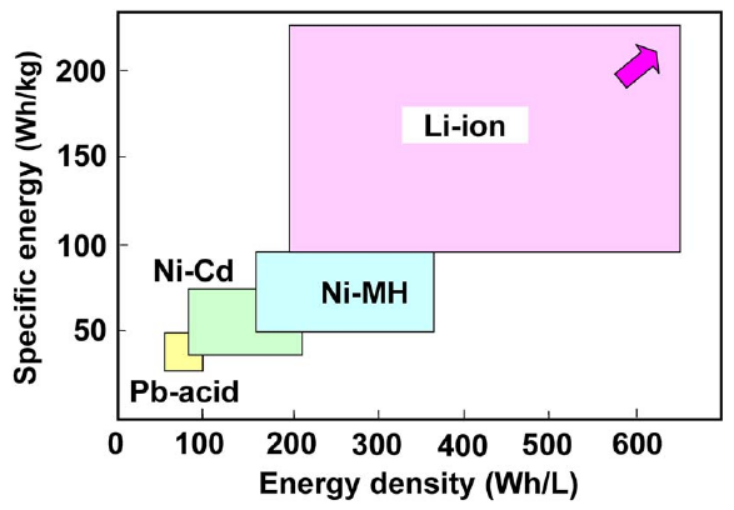
\includegraphics[width=0.6\textwidth]{comparisson-liion.png}
	\caption{Gr\'afica comparativa entre distintas tecnologías de baterías.}
	\label{comparisson_batt}
    \end{center}
\end{figure}

\noindent La aplicación práctica de las baterías de Litio-ion involucra la
integración de las mismas dentro de un sistema, involucrando un controlador
central (\acrshort{BMS}), sistemas de refrigeración, sensores y conectores entre
las celdas. En tales sistemas las celdas pueden conectarse de distintas formas,
por ejemplo, pueden conectarse en paralelo, para incrementar la capacidad del
pack, en serie, para incrementar el voltaje, o combinadas para lograr ambos
cometidos al mismo tiempo. Por ejemplo, un auto eléctrico de la marca
\emph{Tesla}, posee un pack de baterías de 85KWh compuesto por 7104 celdas, con
una arquitectura de 16 módulos conectados en serie , donde cada uno posee 444
celdas conectadas en paralelo.

\newpage

\subsection{Modelado de bater\'ias de litio-ion}\label{litioModel}

\noindent Como se menciona anteriormente, las celdas de litio-ion son utilizadas
ampliamente en el mercado de consumo electr\'onico para un gran espectro de 
aplicaciones. Sin embargo, su fiabilidad y tiempo de vida son limitados y 
depende considerablemente de condiciones ambientales como tambien su uso 
hist\'orico. Por lo tanto, se necesitan modelos de bater\'ias exactos y eficaces 
para que sean correctamente monitoreados por un \acrshort{BMS}.

\noindent Una celda, como se describe en la Secci\'on \ref{battery_fun}, puede 
ser caracterizada como un sistema electrotermoqu\'imico y actualmente existen 
una cantidad numerosa de modelos que logran describir el funcionamiento tanto 
est\'atico como din\'amico de la misma. Un modelo exacto y eficiente permite 
optimizar al m\'aximo el ciclo de vida de una bater\'ia ya que permite 
obtener informaci\'on sobre el \acrshort{SOC} como tambi\'en conocer 
par\'ametros cr\'iticos de la bater\'ia como por ejemplo, el perfil de descarga 
de la misma permitiendo ajustar los distintos algoritmos de protecci\'on y/o 
ecualizaci\'on  que se apliquen en el desarrollo del \acrshort{BMS}.

\noindent A continuaci\'on se definen y se comparan los distintos modelos 
disponibles en la literatura actual. Esta comparaci\'on es basada en tres 
criterios:

\begin{itemize}
    \item \textbf{Precisi\'on}: La precisi\'on define cuan cercano un modelo
        puede predecir los par\'ametros y/o valores de las variables de
        inter\'es de una bater\'ia.
    \item \textbf{Complejidad}: Se refiere a la cantidad de par\'ametros que
        necesita el modelo. Dependiendo de la complejidad del, el c\'alculo 
        del mismo tomara m\'as o menor tiempo, cuestionando su utilidad para una 
        aplicaci\'on en tiempo real.
    \item \textbf{Interpretaci\'on f\'isica}: Esto se define como el nivel de
        interpretaci\'on anal\'itico que el modelo puede dar con respecto al
        funcionamiento interno de una bater\'ia.
\end{itemize}

\subsubsection{Modelos F\'isicos}\label{phyModel}

\noindent O Tambi\'en conocidos como cajas blancas (del ingl\'es, 
\emph{white boxes}), los modelos f\'isicos son modelos de bajo nivel con un 
nivel de exactitud muy alto. Permiten describir la estructura de los materiales 
y logran describir los complejos fen\'omenos electroqu\'imicos que suceden 
dentro de celda, tambi\'en denominados fen\'omenos termodin\'amicos, kin\'eticos 
y de transporte.

\noindent Schmidt (2013) presenta un resumen del fen\'omeno f\'isico como se 
muestra en la Figura \ref{schmidt_fen_fis}. En ella, se pueden observar cuatro 
procesos en tres regiones de operaci\'on: las dos fases s\'olidas del material 
de los electrodos, y la fase l\'iquida del electrolito.

\begin{figure}[h!]
    \begin{center}
        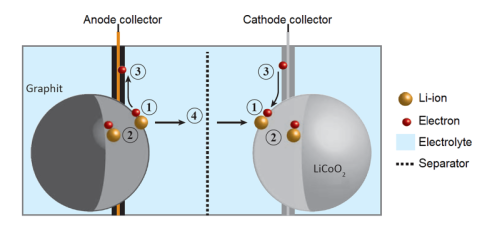
\includegraphics[width=0.7\textwidth]{schmidt_proceso_fisico.png}
        \caption{Descripci\'on gr\'afica del proceso interno de una celda de
        litio ion.}
        \label{schmidt_fen_fis}
    \end{center}
\end{figure}

\noindent El primer proceso se denomina el \emph{pasaje} de cargas y se da en 
la primer regi\'on de operaci\'on: La fase s\'olida del electrodo. 
Este proceso describe la intercalaci\'on como tambi\'en la desintercalaci\'on 
de los iones de litio dentro del material activo. El segundo proceso, ocurren 
en la misma regi\'on, y se la denomina la \emph{difusi\'on del estado s\'olido} 
de los iones de litio forzado por el gradiente de concentraci\'on de iones entre 
la superficie y el volumen del electrodo. El tercer proceso, se describe como 
la \emph{conducci\'on de electrones} entre un electrodo y otro a trav\'es de 
un circuito externo. Por \'ultimo, el cuarto proceso es la \emph{conducci\'on de 
iones} en el electrolito a trav\'es del separador, que tambi\'en es forzado for 
un gradiente de concentraci\'on y basado en la difusi\'on pero ocurre a mucha 
mayor velocidad que en los electrodos.

\noindent Estos tipos de modelos dependen de una gran cantidad de par\'ametros,
como tambi\'en de ecuaciones diferenciales interdependientes, para poder 
replicar el comportamiento de una celda, como por ejemplo, coeficientes de 
difusi\'on y propiedades de los materiales son variables relevantes utilizadas 
en estas ecuaciones. En \cite{Li2016} se basa en un modelo unidimensional a lo
largo de la secci\'on de la celda, dividiendolo en cinco secciones,
aplicando las siguientes ecuaciones diferenciales: 

\begin{itemize}
    \item \textbf{Conservaci\'on de carga en un s\'olido homog\'eneo}
        \begin{equation}
            \nabla (-\sigma\nabla\upvarphi_s)=-j^{Li} 
            \label{Chrg_cons_hom_sol}
        \end{equation}	
    \item \textbf{Conservaci\'on de masa en un s\'olido homog\'eneo}
        \begin{equation}
            \frac{\partial c_s}{\partial t}=\nabla \cdot (D_s\nabla c_s) 
            \label{Mass_cons_hom_sol}
        \end{equation}	
    \item \textbf{Conservaci\'on de masa en un electrolito homog\'eneo}
        \begin{equation}
            \varepsilon_e\frac{\partial c_e}{\partial t} + \nabla \cdot
            (-D_e\nabla c_e) = \left(\frac{1-t_+^0}{F}\right)j^{Li}
            \label{Mass_cons_hom_electrolyte}
        \end{equation}	
    \item \textbf{Conservaci\'on de carga en un electrolito homog\'eneo}
        \begin{equation}
            \nabla \cdot (\upkappa \nabla \upvarphi_e + \upkappa_D \nabla \ln 
            c_e) = -j^{Li}
            \label{Chrg_cons_hom_electrolyte}
        \end{equation}	
    \item \textbf{Ecuaci\'on de Butler-Volmer:} Esta ecuaci\'on representa el
        movimiento de cargas en una uni\'on entre un s\'olido conductor y una
        soluci\'on de iones de litio con el efecto de doble capa
        \begin{equation}
            j^{Li} =
            a_si_0\left[{e^\frac{F\eta}{2RT}-e^{-\frac{F\eta}{2RT}}}\right] + 
            a_sC_{dl}\frac{\partial{(\upvarphi_s - \upvarphi_e)}}{\partial t}
            \label{Butler_Volmer_kinetics}
        \end{equation}	
\end{itemize}

\noindent En las ecuaciones \ref{Chrg_cons_hom_sol} - 
\ref{Butler_Volmer_kinetics}, se utilizan las siguientes variables:

\begin{itemize}
    \item $\mathrm{\sigma}$: Conductividad de la fase s\'olida del
        electrodo.
    \item $\mathrm{\upvarphi_s}$: Potencial el\'ectrico de la fase
        s\'olida.
    \item $\mathrm{\upvarphi_e}$: Potencial el\'ectrico del
        electrolito.
    \item $\mathrm{j^{Li}}$: Densidad de corriente producida por el
        consumo de iones de litio.
    \item t: Tiempo transcurrido.
    \item c: Concentraci\'on de iones de litio.
    \item D: Coeficiente de difusi\'on del material.
    \item F: Constante de Faraday.
    \item $\mathrm{\varepsilon}$: Fracci\'on por volumen.
    \item $\mathrm{t_+^0}$: N\'umero de transferencia.
    \item $\mathrm{\upkappa}$: Conductividad del electrolito.
    \item $\mathrm{\upkappa_D}$: Conductividad de la difusi\'on.
    \item $\mathrm{i_0}$: Corriente de intercambio.
    \item $\mathrm{\eta}$: Sobretensi\'on.
    \item a: \'Area espec\'ifica de la secci\'on.
    \item $\mathrm{C_{dl}}$: C\'apacidad de la doble capa.
\end{itemize}

A pesar de su alta exactitud, este tipo de modelo resulta complejo de
implementar en sistemas de tiempo real debido a la gran cantidad de ecuaciones
diferenciales a implementar con su extensa cantidad de par\'ametros a ajustar en
el mismo, imposibilitando su uso en veh\'iculos el\'ectricos.

\subsubsection{Modelos emp\'iricos}\label{empModels}

\noindent Los modelos emp\'iricos, o tambi\'en conocidos como 
\emph{cajas negras}, debido a que proveen pobres conocimientos sobre el 
funcionamiento interno del sistema, se basan en par\'ametros emp\'iricos que no 
tienen ning\'un significado f\'isico en algunos casos. 
Las aproximaciones matem\'aticas que se utilizan para definir la
funci\'on transferencia entre las entradas y las salidas de estos modelos
permiten que los mismos sean f\'aciles de configurar como tambi\'en generar
predicciones y respuestas r\'apidas. Sin embargo, la exactitud es limitada,
especialmente si el modelo es muy simple, aunque puede ser mejorado si se combina
con un modelo de bajo nivel.

\subsubsection{Modelos abstractos}\label{absModels}

\noindent Tambi\'en conocidos como \emph{cajas grises}, los modelos abstractos 
proveen una representaci\'on alternativa de la entidad f\'isica a modelar. 
A pesar de que hay varias formas posibles de realizarlo, la m\'as utilizada 
dentro de la bibliograf\'ia es su representaci\'on en un circuito el\'ectrico 
equivalente. Los modelos basados en circuitos son simples y pr\'acticos porque 
permiten que el proceso electroqu\'imico que ocurre dentro de la celda sea 
reemplazado por un simple circuito. La correlaci\'on con las din\'amicas de la 
bater\'ia son preservados sin comprometer demasiada exactitud en su 
predicci\'on.

\noindent El costo de configuraci\'on para tales modelos es reducido en 
comparaci\'on a modelos de bajo nivel, sin embargo \'estos requiren de 
\emph{Look-up Tables} para coincidir con los datos experimentales. 
La complejidad de los mismos es m\'as flexible dependiendo de la unidad de 
c\'omputo como tambi\'en de la memoria disponible. Los mismo se pueden 
acomplejizar utilizando efectos de segundo \'orden, tales como la temperatura, 
degradaci\'on de la capacidad como tambi\'en el envejecimiento de las celdas.

\noindent A continuaci\'on se describen los modelos m\'as utilizados dentro de 
la literatura actual.

\subsubsubsection{Circuito simple}

\noindent El circuito el\'ectrico mas simple que representa una bater\'ia de 
litio ion es un circuito con constante de tiempo cero que se puede observar en 
la Figura \ref{zero_time_constant_sch}. Si el usuario no necesita representar la 
din\'amica de la bater\'ia, este modelo es capaz de representar el 
comportamiento est\'atico del sistema. 

\begin{figure}[h!]
    \begin{center}
        \begin{circuitikz}[american voltages]
            \draw 
                (0, 0) -- (3.5, 0)
                (0, 0) -- (0, .5)
                (0, 1.5) to[american voltage source, v_=$V_{OCV}$] (0, 0.5)
                (0, 1.5) -- (0, 2) to[R, l_=$R_S$] (3, 2) 
                to [short, i_=$I_{batt}$] (3.5, 2)
                (4, 2) to [open, v=$V_{batt}$] (4, 0);
        \end{circuitikz}
        \caption{Modelo de constante de tiempo cero para una celda de litio 
                 ion.}
        \label{zero_time_constant_sch}
    \end{center}
\end{figure}


\noindent El \acrshort{OCV} se relaciona directamente con el \acrshort{SOC},
definido en la Ecuacion \ref{ocv_soc_ztc}

\begin{equation}
    SoC = \frac{C_{current}}{C_{full}}\dot 100\% \label{ocv_soc_ztc}
\end{equation}

\noindent Donde $\mathrm{C_{current}}$ es la cantidad de carga disponible en la 
celda y $\mathrm{C_{full}}$ es la capacidad de la celda cuando est\'a 
completamente cargada. La ecuaci\'on del modelo es expresada en la Ecuaci\'on 
\ref{vbatt_ocv_soc_ztc}.

\begin{equation}
    V_{batt} = V_{OC} - R_S \times I_{batt} \label{vbatt_ocv_soc_ztc}
\end{equation}

\noindent La curva del \acrshort{OCV} como funci\'on del tiempo muestra una 
caida del voltage para ciertas condiciones de descarga. Los importantes 
par\'ametros que afectan el proceso de descarga son la corriente de descarga, 
la temperatura y el historia de carga/descarga.

\noindent El efecto de la temperatura en el efecto de descarga es visto a
temperaturas mucho mas bajas que a temperatura ambientes, donde la actividad
qu\'imica disminuye y la resitencia de la bater\'ia aumenta. A temperaturas
m\'as altas que la ambiente, la resistencia interna disminuye, mejorando la
velocidad de la actividad qu\'imica, por lo tanto, y desafortunadamente,
induciendo un efecto de auto descarga.

\noindent La desventaja principal del modelo de constante de tiempo cero es que 
no contempla la din\'amica de las celdas. Sin embargo, esto puede ser mitigado 
de forma f\'acil agregando un tanque RC en serie a la resistencia (\emph{fig.
\ref{one_time_constant_sch}}), que describe la respuesta din\'amica de la 
bater\'ia durante el proceso de carga/descarga.

\begin{figure}[h!]
    \begin{center}
        \begin{circuitikz}[american voltages]
            \draw 
                (0, 0) -- (7, 0)
                (0, 0) -- (0, 1)
                (0, 2) to[american voltage source, v_=$V_{OCV}$] (0, 1)
                (0, 2) -- (0, 3) to[R, l_=$R_s$] (3, 3) to[R, l_=$R_p$] (6, 3)
                (3, 3) to[short, *-] (3, 1.5) to [C, l_=$C_p$] 
                (6, 1.5) -- (6, 3) to [short, i_=$I_{batt}$] (7, 3)
                (7.5, 3) to [open, v=$V_{batt}$] (7.5, 0);
        \end{circuitikz}
        \caption{Modelo de primer \'orden para una celda de litio ion.}
        \label{one_time_constant_sch}
    \end{center}
\end{figure}

\noindent La exactitud del modelo y su comportamiento din\'amico, pueden ser 
mejorados agregando m\'as tanques RC al circuito, esto a su vez incrementa la
complejidad del mismo. 

\subsubsubsection{Modelos basados en el espectro de impedancia}

\noindent Para describir la din\'amica de una celda a niveles de medianas y 
altas frecuencias, se utiliza el m\'etodo de impedancia electroqu\'imica por 
espectroscop\'ia (\acrshort{EIS}, del ingl\'es \acrlong{EIS}). Sin embargo, para
aplicar este m\'etodo, es necesario un sistema lineal invariante en el tiempo,
por lo tanto, dado que las bater\'ias son sistemas altamente no lineales durante
el proceso de carga y descarga, el \acrshort{EIS} es aplicado a dados niveles de
\acrshort{SOC} cuando la bater\'ia tiene un determinado tiempo de descanso, para
garantizar determinada linealidad necesaria.

\noindent La impedancia (Z) es una variable compleja representada en en el 
diagrama de Nyquist por una componente real y otra imaginaria. 
La Figura \ref{EIS_Nyquist} muestra un t\'ipico diagrama de Nyquist, 
resultado de mediciones \acrshort{EIS} de una celda de litio-ion. 
Cuantitativamente, los valores dependen de varios factores, como mencionamos 
anteriormente, la temperatura, el \acrshort{SOC} y la corriente de carga.

\begin{figure}[h!]
    \begin{center}
	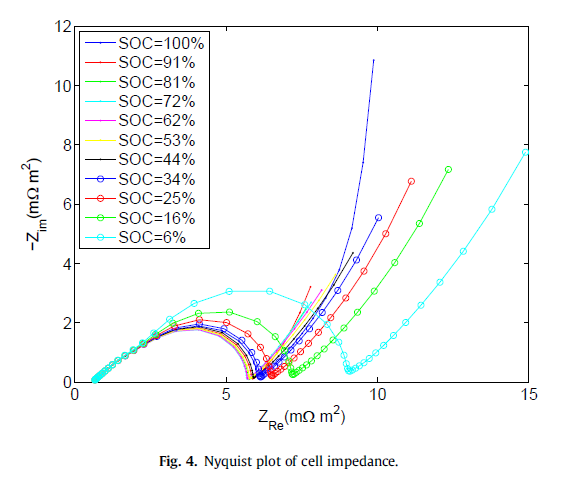
\includegraphics[width=0.4\textwidth]{EIS_Nyquist.png}
	\caption{Diagrama de Nyquist - Espectroscopía Dieléctrica (EIS) de 
	una batería de Li-Ion obtenida por barrido frecuencial.}
	\label{EIS_Nyquist}
    \end{center}
\end{figure}

\newpage

\noindent La curva puede ser subdividida seg\'un los rangos de frecuencia en
distintas secciones, como se puede observar en la Figura
\ref{EIS_nyquist_sections}. Estas secciones se pueden asociar con fen\'omenos 
f\'isicos y electroqu\'imicos bien definidos que ocurren dentro de la celda.

\begin{figure}[h!]
    \begin{center}
	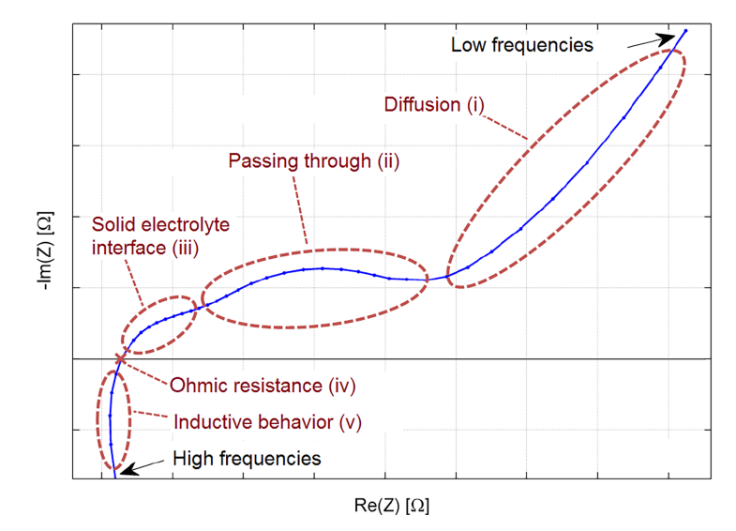
\includegraphics[width=0.7\textwidth]{EIS_nyquist_section.png}
	\caption{Secciones identificables dentro del diagrama de Nyquist.}
	\label{EIS_nyquist_sections}
    \end{center}
\end{figure}

\noindent La secci\'on con $\mathrm{Z" < 0}$ consiste de tres \'areas bien 
reconocibles. El arco a frecuencies muy bajas (cercanas a DC) se asocia con el 
comportamiento de difusi\'on introducido en la Seccion \ref{battery_fun} y es 
representado por la impedancia de \emph{estado s\'olido de Warburg}. El segundo 
arco a frecuencias un poco m\'as altas (arco [ii] en Fig. 
\ref{EIS_nyquist_sections}) corresponde a la kin\'etica de la transferencia de 
carga. El tercer y arco m\'as pequeño arc cerca del eje real (arco [iii] en Fig. 
\ref{EIS_nyquist_sections}) representa los efectos entre capas de la interface 
s\'olida del electrolito.

\noindent El punto (iv) de la Figura \ref{EIS_nyquist_sections} representa la 
resistencia \'ohmica total del sistema, incluyendo la resistencia del 
electrolito como tambi\'en la de los electrodos. Este punto generalmente occurre 
a una frecuencia dentro del rango de los KHz pero puede variar considerablemente 
con el diseño de la celda y los materiales utilizados.

\noindent Las altas frecuencias muestran un comportamiento inductivo con 
$\mathrm{Z" > 0}$ (secci\'on (v) de la Figura \ref{EIS_nyquist_sections}) 
correspondiente a la estructura porosa de los electrodos y los conectores de la 
bater\'ia.

\noindent El circuito equivalente de la respuesta de la impedancia es
introducido por Moss et al. (2008) y se puede observar en la Figura
\ref{sch_modelo_EIS}

\begin{figure}[h!]
    \begin{center}
        \begin{circuitikz}
            \draw
            (0, 0) to[L, o-, l=$L_s$] (2, 0) to [R, l=$R_s$] (4, 0) to[R,
            l=$R_{p1}$] (6, 0)
            (4, 0) to [short, *-] (4, -2) to [C, l=$C_{p1}$] (6, -2) to [short, -*]
            (6, 0) to[short, -*] (7, 0) to [C, l=$C_{dl}$] (11, 0)
            (7, 0) to[short] (7, -2) to[R, l=$R_{CT}$] 
            (9, -2) to[R, l=$Z(\omega)$] (11, -2) to[short, -*] (11, 0)
            to[C, -o, l=$C_{int}$] (12, 0);
        \end{circuitikz}
        \caption{Modelo equivalente a la respuesta del \acrshort{EIS}}
        \label{sch_modelo_EIS}
    \end{center}
\end{figure}

\noindent Donde los componentes representan las siguientes partes f\'isica de 
la celda:

\begin{itemize}
    \item $\mathrm{C_{dl}}$: Es la capacitancia electroqu\'imica de doble capa
        de la celda.
    \item $\mathrm{R_{CT}}$: Es la resistencia a la corriente
        far\'adica
    \item $\mathrm{C_{int}}$: Es la capacitancia de intercalaci\'on
        correspondiente a la acumuluaci\'on de iones de litio dentro de la
        matriz del electrodo.
    \item $\mathrm{Z(\omega)}$: Es la impedancia de estado s\'olido de Warburg
        que depende de la frecuencia del ensayo.
\end{itemize}

\noindent Moss et al. (2008) sugiere la substituci\'on de la impedancia de 
difusi\'on de Warburg con una cadena de tanques RC. La nueva cadena no refleja 
la impedancia del elemento de warburg pero representa una aproximaci\'on con una 
exactitud aceptable. Tomando esta aproximaci\'on en consideraci\'on, se valida 
el uso de modelos el\'ectricos para modelar celdas en un circuito compuesto 
por una fuente de tensi\'on con una resistencia $\mathrm{R_s}$ y una cadena de 
tanques RC conectadas en serie. Esto es solo posible gracias a las relaciones de 
Kramers-Kronig (Schmidt, 2013), que pueden ser aplicadas en redes equivalentes, 
y sugiere que distintos circuitos pueden tener una respuesta equivalente o 
similar sin tener la misma topolog\'ia. En otras palabras, la bater\'ia puede 
ser modelada con una topolog\'ia m\'as simple con elementos de circuito que no 
tienen una directa interpretaci\'on f\'isica. Este modelo es v\'alido, porque 
tiene la misma respuesta en frecuencia, y es m\'as f\'acil de parametrizar.

\subsubsection{Comparaci\'on de modelos y su evaluaci\'on para aplicaciones
en veh\'iculos el\'ectricos}\label{compModels}

\noindent La Tabla \ref{table_comp_models} presenta un vistazo general sobre la
comparaci\'on de los modelos seg\'un el criterio previamente explicado. Los
modelos simples pueden ser menos costosos desde un punto de vista computacional
como tambi\'en en desarrollo, a su vez, \'estos son mas susceptibles a
incertezas en los par\'ametros del mismo. Por el otro lado, modelos complejos
necesitan mayor tiempo para resolver los algoritmos inherentes a ellos.
Dependiendo de la aplicaci\'on, la extracci\'on del m\'etodo del modelo y
usabilidad deben ser evaluados antes de comenzar su desarrollo. 
Dentro de un ambiente de laboratorio, se puede invertir m\'as tiempo para 
extraer un modelo m\'as preciso. Sin embargo, en el campo se necesitan 
resultados de forma r\'apida para evaluar si las celdas son aptas para ser 
aplicadas en un veh\'iculo, por ejemplo, en estos casos los modelos son 
utilizados para el desarrollo de un \acrshort{BMS} como es lo que se busca en el 
presente trabajo. 

\noindent Tener una extensa comprensi\'on de la bater\'ia en estos casos no es
necesario, aunque puede resultar beneficioso. Dado que el mismo es embebido
dentro de una unidad de monitoreo en tiempo real, tal como un \acrshort{MCU} y/o
\acrshort{FPGA}. Es m\'as conveniente que el modelo sea simple, para que los
tiempos de c\'omputo no sean muy altos comprometiendo niveles aceptables de
exactitud en los mismos. 

\begin{table}[h!]
\begin{center}
\begin{tabular}{@{}ccccc@{}}
\textbf{Modelos} & \textbf{Exactitud} & \textbf{Complejidad} &
\textbf{Interpretaci\'on f\'isica} & \textbf{Aplicaci\'on apropiada}\\
\hline
F\'isicos   & Muy alta  & \textgreater{}50 par\'ametros         & Alta
& diseño de de bater\'ias \\\hline Emp\'iricos & Media 
& 2 a 3 par\'ametros & Baja & Predicciones\\ 
\hline Abstractos & Media & 2 a 30 par\'ametros & Limitada & 
Monitoreo y diagn\'ostico
\end{tabular}
\caption{Resumen de la comparaci\'on entre modelos de celdas de litio-ion.}
\label{table_comp_models}
\end{center}
\end{table}

\subsection{Algoritmos de Estimaci\'on del Estado de Carga}\label{algSoc}

\noindent El \acrshort{SOC} es el equivalente a medir la cantidad de combustible
restante en un veh\'iculo convencional basado en combustibles f\'osiles. La
funci\'on principal de esta variable es comunicar de forma instintiva el estado
de la bater\'ia al conductor y, al mismo tiempo, evitar problemas tales como la
sobrecarga y sobredescarga del pack de bater\'ias, en otras palabras, mantener
el pack de bater\'ia dentro de la zona de operaci\'on segura como tambi\'en 
lograr mantener las celdas ecualizadas entre si.

\noindent \'Esta tarea involucra el uso de sensores que permitan obtener las
señales de tensi\'on, corriente y temperatura de la bater\'ia para que el
circuito de control pueda procesarlos y computar el \acrshort{SOC},
usando uno de los algoritmos disponibles en la literatura actual que 
un tema que se encuentra en constante investigaci\'on debido al funcionamiento 
no-lineal de las celdas de litio ion inherentes a sus elementos 
electroqu\'imicos, que se  ven afectados por condiciones internas y externas.

\newpage

\noindent Cuando se menciona el \acrshort{SOC}, se refiere a la relaci\'on entre
la capacidad de corriente que queda en la bater\'ia con respecto a la capacidad
total bajo determinadas condiciones (temperatura, corriente de carga/descarga,
envejecimiento, entre otras), y su expresi\'on matem\'atica se puede observar en
la Ecuaci\'on \ref{eq_soc_int}

\begin{equation}
    SOC = \frac{Q_c}{Q}\times100\% 
    \label{eq_soc_int}
\end{equation}

\noindent Donde, desde el punto de vista de los veh\'iculos el\'ectricos,
$\mathrm{Q_c}$ es la energia residual de la bater\'ia en el momento que se
calcula, y su unidad es Ah (Ampere-hora); Q es la capacidad total de la
bater\'ia teniendo la misma unidad que $\mathrm{Q_c}$.

\noindent El hecho de que la bater\'ia dependa de varios factores, obliga a que
la Ecuaci\'on \ref{eq_soc_int} sea modificada, obteniendo la siguiente 
expresi\'on (\emph{eq. \ref{eq_soc_extended}}).

\begin{equation}
    SOC(t) = SOC(t_0) - \int_{t_0}^t \frac{\eta I}{C_n }d\tau
    \label{eq_soc_extended}
\end{equation}

\noindent En la Ecuaci\'on \ref{eq_soc_extended}, $\mathrm{C_n}$ es la 
capacidad nominal de la bater\'ia (en Ah), $\mathrm{\eta}$ es la eficiencia 
cul\'ombica de la celda e I es la corriente que circula sobre la celda en el 
instante de tiempo t.

\noindent Adem\'as del comportamiento de la celda, tambi\'en se debe modelar el
efecto de envejecimiento de la celda sobre el estado de carga, que puede ser
afectado por el ensamblado de la bater\'ia, temperatura, condiciones de
ventilaci\'on, corriente de auto-descarga, concentraci\'on de electrolitos, por
el otro lado, tambi\'en se lo relaciona con inconsistencias entre las distintas
celdas que componen el pack de bater\'ias, como por ejemplo, voltaje,
resistencia interna, capacidad y otros par\'ametros que afectan el 
envejecimiento del pack. La relaci\'on del envejecimiento y el \acrshort{SOC} se
ve reflejado por el \acrshort{SOH}, que es una variable que permite cuantificar
la antigüedad de una bater\'ia. La influencia del envejecimiento de la celda
sobre el \acrshort{SOC} se puede expresar en la Ecuaci\'on \ref{soc_soh}.

\begin{equation}
    SOC(t) = SOH(t) - DOD(t) \label{soc_soh}
\end{equation}

\noindent En la Ecuaci\'on \ref{soc_soh}, SOH(t) es el estado de salud. 
Cuando la bater\'ia es nueva, se considera que el SOH est\'a a un 100\%. 
Por el otro lado, el \acrshort{DOD} (del ingl\'es, \acrlong{DOD}) indica cuanto 
de la capacidad total de la bater\'ia puede ser descargado realmente, este valor 
se toma en cuenta cuando solo se puede descargar el 80\% de la capacidad total 
de la celda.

\noindent Basado en caracter\'isticas experimentales y te\'oricas, existen 
varios m\'etodos para estimar el \acrshort{SOC} y pueden ser clasificados dentro 
de tres grupos: Los m\'etodos tradicionales de estimaci\'on que se basan 
meramente en datos experimentales, m\'etodos modernos basados en teor\'ias de 
control y, por \'ultimo, m\'etodos basados novedosos basados en algoritmos
pertenecientes a lo que hoy se denomina la \emph{ciencia de datos}.

\subsubsection{M\'etodos tradicionales basados en experimentos}
\label{tradSocMeth}

\subsubsubsection{M\'etodo en base al voltaje de circuito abierto}
\label{ocv_section}

\noindent La medici\'on del voltaje de circuito abierto, u \acrshort{OCV}, se
basa en la relaci\'on entre la medici\'on de este voltage y el \acrshort{SOC}
representado en la Ecuaci\'on \ref{ocv_soc_eq}.

\begin{equation}
    V_{OC} = f(SOC) \label{ocv_soc_eq}
\end{equation}

\noindent Esta relaci\'on se determina realizando el experimento \acrshort{HPPC} 
(del ingl\'es, \acrlong{HPPC}) que consiste en descargar la bater\'ia con pulsos 
de corrientes equivalentes a un tercio de su capacidad comenzando desde el 
100\% de la bater\'ia hasta un 10\% de su capacidad en donde, despu\'es de cada 
pulso, se deja descansar a la celda por un un intervalo de 2 horas, permitiendo 
que la misma se equilibre de forma t\'ermica y electroqu\'imica antes de aplicar 
el pr\'oximo pulso de corriente. Durante el proceso de este ensayo, se toman 
mediciones de corriente y tensi\'on en bornes de la bater\'ia, permiti\'endo 
obtener una curva de \acrshort{OCV} vs \acrshort{SOC} como se puede observar en 
la Figura \ref{soc_ocv_paper}.

\begin{figure}[h!]
    \begin{center}
        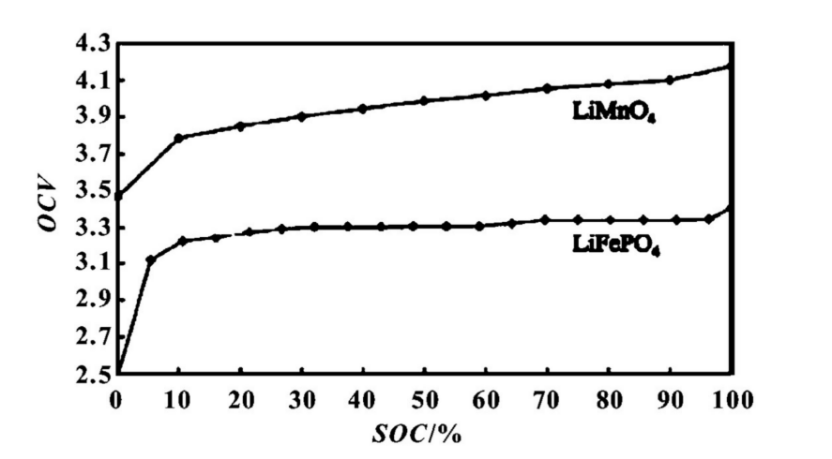
\includegraphics[width=0.6\textwidth]{soc_ocv_paper.png}
        \caption{Curva \acrshort{OCV} vs \acrshort{SOC} de una celda de hierro
        litio fosfato y otra de litio \'acido manganeso.}
        \label{soc_ocv_paper}
    \end{center}
\end{figure}

\noindent La ventaja del m\'etodo basado en la medici\'on del \acrshort{OCV} es
que es muy simple de implementar, solo hace falta tener una lectura de la
tensi\'on en bornes de la celda. Sin embargo, a pesar de su simpleza, el
m\'etodo no es apto para realizar una estimaci\'on en tiempo real debido a las
din\'amicas internas de la celda.

\noindent Por ejemplo, el voltage de la celda tiene una respuesta muy din\'amica
ante fluctuaciones de corriente, como se puede observar en la Figura
\ref{relaxation_ocv}, lo que imposibilita utilizar este m\'etodo como estimador
del \acrshort{SOC} en tiempo real, ya que ante una pequeña circulaci\'on de
corriente la correlaci\'on entre el voltaje y el \acrshort{SOC} no es directa.

\begin{figure}[h!]
    \begin{center}
        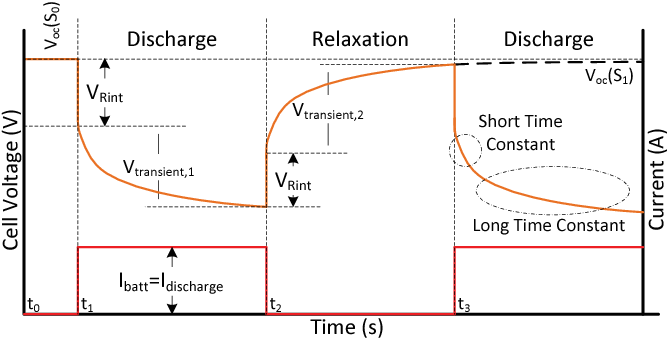
\includegraphics[width=0.7\textwidth]{ocv_relaxation.png}
        \caption{Repuesta de la tensi\'on de salida de una celda de Litio-ion
        ante un escal\'on de corriente}
        \label{relaxation_ocv}
    \end{center}
\end{figure}

\noindent Por el otro lado, las celdas de litio-ion poseen un voltage de
hist\'eresis en el proceso de carga y descarga, como se puede observar en la
Figura \ref{histeresis_plot}, donde en la misma se muestrea el \acrshort{SOC}
para distintos per\'iodos de relajaci\'on, en ella se puede notar como
afecta el per\'iodo de relajaci\'on para realizar la estimaci\'on, donde a
mayor tiempo mejor es la estimaci\'on, esto es directamente relacionado con la
difusi\'on del litio dentro de la celda.

\begin{figure}[h!]
    \begin{center}
        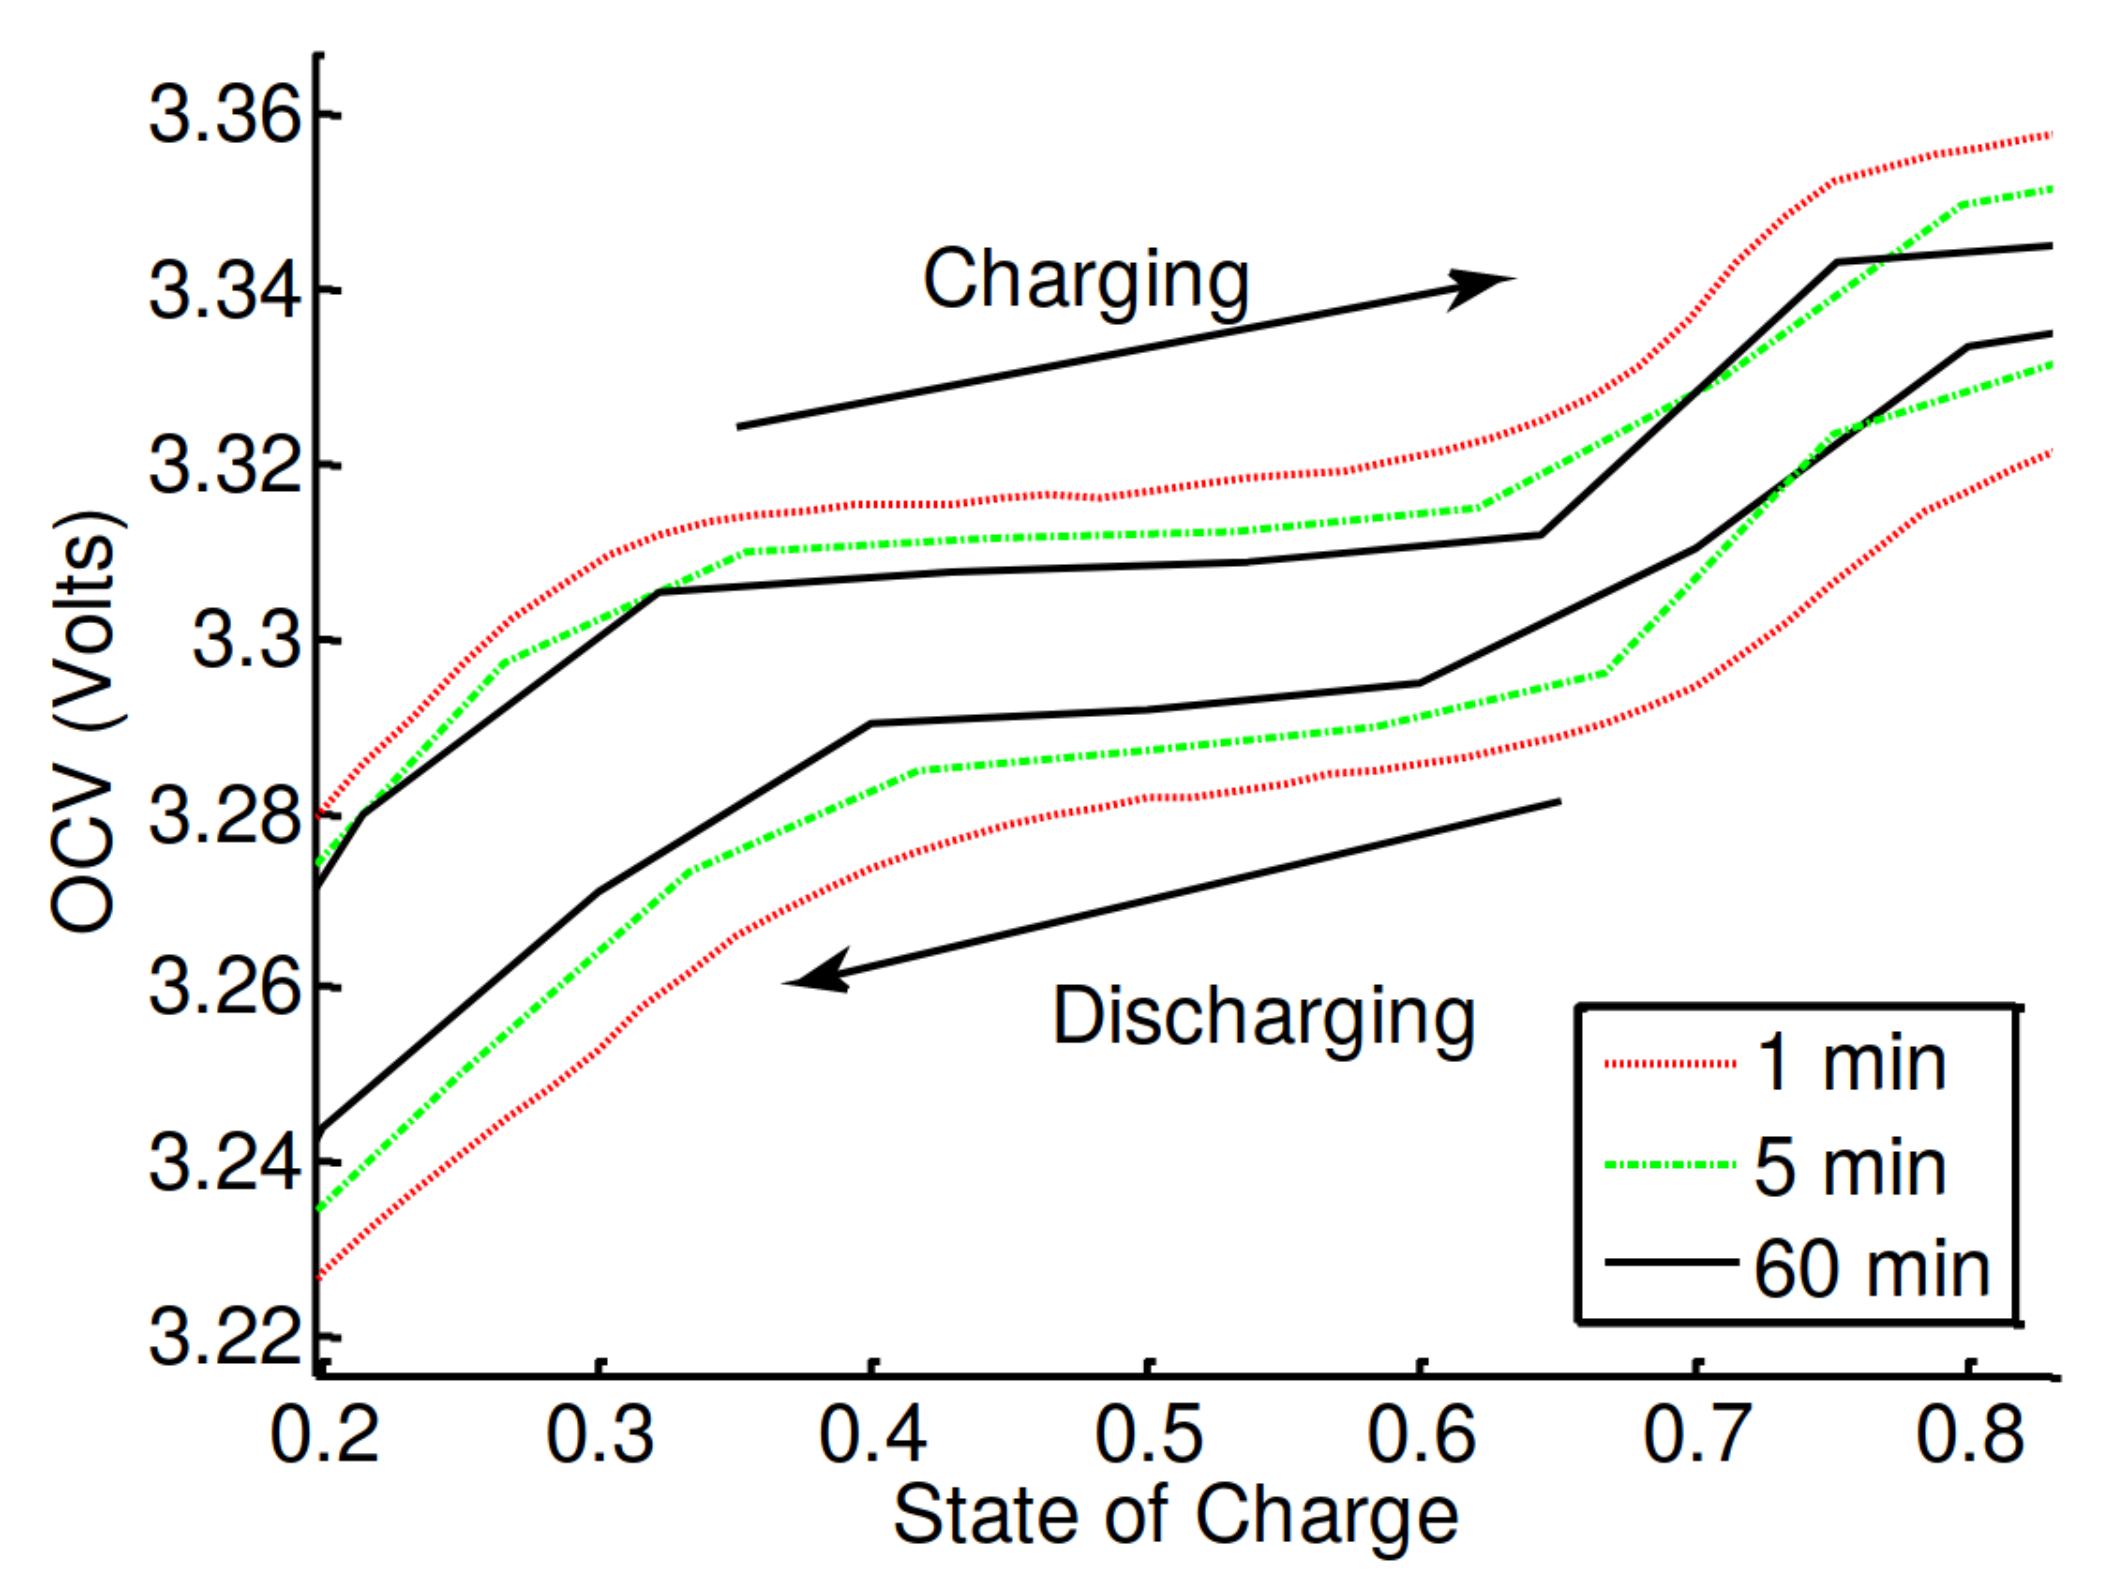
\includegraphics[width=0.5\textwidth]{soc_histeresis.png}
        \caption{\acrshort{OCV} vs \acrshort{SOC} mostrando la variaci\'on del
        voltaje ante la variaci\'on del tiempo de descanso} 
        \label{histeresis_plot}
    \end{center}
\end{figure}

\noindent Finalmente, la curva \acrshort{OCV} vs \acrshort{SOC} de la Figura
\ref{soc_ocv_paper} muestra secciones en la que la señal del \acrshort{OCV} es
plana ante una variaci\'on del \acrshort{SOC}, particularmente entre el 40\% y
el 60\%. Adem\'as, hay una variaci\'on muy pequeña en tensi\'on entre el 20\% y
80\%, lo cual, ante un m\'inimo error en la lectura de la tensi\'on de la celda
puede llevar a mediciones muy inexactas del \acrshort{SOC}. Estas observaciones
son los principales retos de estimar el \acrshort{SOC} utilizando solamente la
medici\'on del \acrshort{OCV}, lo cual llev\'o al desarrollo de nuevas
metodolog\'ias de estimaci\'on.

\newpage

\subsubsubsection{M\'etodo de integraci\'on de corriente}\label{ahMethod}

\noindent \'Este m\'etodo es utilizado com\'unmente para medir la corriente
el\'ectrica acumulada/entregada en determinado per\'iodo de tiempo. Se basa en
el c\'alculo de la circulaci\'on de corriente acumulada durante el proceso de
carga y descarga de una bater\'ia. En la literatura se plantean varias versiones
de una descripci\'on matem\'atica de este m\'etodo, la m\'as utilizada se
puede describir en la Ecuaci\'on \ref{ah_soc_general}.

\begin{equation}
    SOC = \frac{Q_0 + \int_{0}^t i_c\eta dt - \int_{0}^t i_d dt - S}{Q}
    \label{ah_soc_general}
\end{equation}

\noindent En la Ecuaci\'on \ref{ah_soc_general}, Q es la capacidad total de la 
bater\'ia, $\mathrm{Q_0}$ es la carga inicial de la celda, $\mathrm{\eta}$ es la 
eficiencia de carga, S es la cantidad estimada de auto-descarga de la celda, 
$\mathrm{i_c}$ es la corriente de carga e $\mathrm{i_d}$ es la corriente de 
descarga.

\noindent Por el otro lado, en la literatura tambi\'en se encuentran versiones
mejoradas de \'este m\'etodo para corregir el error estimado. El principio de
operaci\'on se puede observar en la Ecuaci\'on \ref{ah_soc_enhanced}.

\begin{equation}
    SOC = \alpha SOC_0 - \frac{1}{\delta c}\int \eta_\epsilon I dt
    \label{ah_soc_enhanced}
\end{equation}

En esta ecuaci\'on, $\mathrm{SOC_0}$ es obtenida por el m\'etodo de
\acrshort{OCV} descripto en la Secci\'on \ref{ocv_section}, $\mathrm{\alpha}$ es
el coeficiente que representa el factor de correcci\'on de auto-descarga y
envejecimiento de la celda, que se obtiene en base a varios experimentos en la
celda, $\mathrm{\delta}$ es el factor de correcci\'on por la capacidad de la
bater\'ia que se puede obtener a partir de la Ecuaci\'on
\ref{batt_cap_correction}. El par\'ametro $\mathrm{\eta_\epsilon}$ es la
eficiencia cul\'ombica equivalente de la celda, cuyo valor se obitene unificando
la eficiencia cul\'ombica de distintas corrientes.

\begin{equation}
    \delta = 0.0010N^2 - 0.032N + 11.8819\label{batt_cap_correction}\;
    \text{donde N es el n\'umero de ciclos}
\end{equation}

\noindent El m\'etodo de integraci\'on de corriente tiene la ventaja de ser un
c\'alculo simple, estable y permite ser implementado en tiempo real.
Considerando la auto-descarga, temperatura, eficiencia de carga y descarga, el
m\'etodo puede alcanzar niveles de exactitud aceptables para una
implementaci\'on r\'apida para la estimaci\'on del \acrshort{SOC} en un BMS. Sin
embargo, este m\'etodo tiene dos principales desventajas:

\begin{enumerate}
    \item Dado que solo se integra corriente en un largo per\'iodo de tiempo, el
        m\'etodo es propenso a acumular una considerable cantidad de error en el
        tiempo.
    \item El mismo no logra eliminar la p\'erdida de la capacidad de carga como
        consecuencia del envejecimiento de la celda, logrando que se acumule
        error por cada ciclo de carga.
\end{enumerate}

\noindent Por esto mismo, varias bibliograf\'ias proponen fusionar el m\'etodo
por \acrshort{OCV} junto a \'este para compensar los errores inherentes, as\'i
obteniendo una metodolog\'ia simple y eficiente para estimar el \acrshort{SOC}
de una celda.

\subsubsubsection{Medici\'on de resistencia interna}\label{internalRMethod}

\noindent \'Este m\'etodo tiene el objetivo de relacionar la resistencia interna
de una celda con el \acrshort{SOC}, considerando la corriente de descarga y la
resistencia interna de la bater\'ia. Sin embargo, en la pr\'actica, la
relaci\'on entre los par\'ametros de una celda y el \acrshort{SOC} es bastante
compleja. En la etapa inicial de la descarga, la eficiencia de descarga de la
resistencia interna es estable y su fluctuaci\'on es casi impercetible. Sin
embargo, en la etapa final, la resistencia interna aumenta considerablemente
obteniendo como resultado grandes fluctuaciones, denotando que este m\'etodo es
generalmente aplicado en esta etapa del proceso de descarga. Este comportamiento
se puede observar en la Figura \ref{res_int_graph}.

\begin{figure}[h]
    \begin{center}
	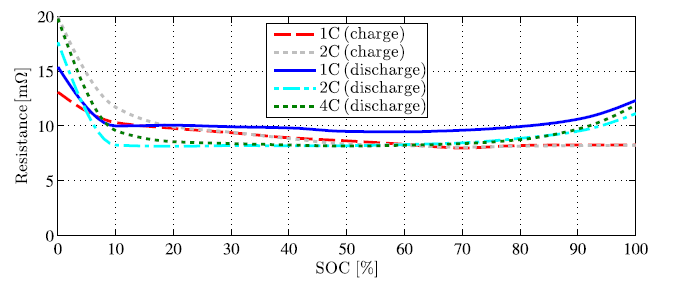
\includegraphics[width=0.7\textwidth]{Ro_vs_SOC.png}
	\caption{Resistencia en corriente continua de una batería de litio ion vs. 
        SOC obtenida por HPPC}
	\label{res_int_graph}
    \end{center}
\end{figure}

\noindent La resistencia interna de una bater\'ia puede ser dividida en la
resistencia de corriente alterna y corriente continua. Por lo tanto,
\'este m\'etodo puede ser dividido en dos m\'etodos para cada uno. 
La impendancia en alterna es la funci\'on transferencia entre el
voltage y la corriente de la celda cuando se le aplica una corriente
alterna y ambos pueden ser medidos f\'acilmente con un medidor de impedancias. 
Sin embargo, a pesar de ser un m\'etodo muy simple de implementar, la relaci\'on 
de la resistencia interna con el SOC se acomplejiza dependiendo de la 
tecnolog\'ia de la bater\'ia, especialmente en las celdas de litio ion.

\noindent El m\'etodo consiste en excitar la bater\'ia breves instantes 
(menores a 10ms) un pulso de corriente, asumiendo que este per\'iodo es lo 
suficientemente acotado para que la variaci\'on de tensi\'on sea atribuida a la 
resistencia interna y no a la carga/descarga de la bater\'ia, el c\'alculo de la 
resistencia se podr\'ia obtener seg\'un la Ecuaci\'on
\ref{rint_batt_eq}:

\begin{equation}
    \frac{\Delta V}{\Delta I} = R_{\ohm} \label{rint_batt_eq}
\end{equation}

Sin embargo, a pesar de su simpleza, este m\'etodo no resulta atractivo para
implementar en sistemas en tiempo real dado que, como se menciona anteriormente,
tiene una gran exactitud \'unicamente en bajos valores de \acrshort{SOC},
adem\'as, tambi\'en debe inyectarse un valor de corriente conocido para poder
estimar su valor, resultando en mayor complejidad al circuito del \acrshort{BMS}
para poder generar este valor de corriente conocido en tiempo real.

\noindent En resumen, los m\'etodos de estimaci\'on del \acrshort{SOC} basados
en experimentos tienen la ventaja de ser simples y f\'aciles de implementar,
pero requieren de mucha inversi\'on experimental en las celdas para un bajo
rendimiento en estimar de forma exacta el \acrshort{SOC}. Con respecto a la
exactitud de estimaci\'on y caractter\'isticas de los ensayos de cada m\'etodo,
se puede decir que:

\begin{itemize}
    \item \textbf{Estimaci\'on por OCV:} La exactitud de \'este m\'etodo depende
        exclusivamente del tiempo en el que la bater\'ia estuvo relajada,
        mientras mayor sea este tiempo m\'as exacto es la estimaci\'on.
    \item \textbf{Estimaci\'on por integraci\'on de corriente:} Es
        principalmente utilizado para determinar el \acrshort{SOC} inicial, pero
        si exactitud disminuye con el tiempo de medici\'on, debido a que la
        resistencia interna cambia constantemente y es propenso a acumular
        errores.
    \item \textbf{M\'etodo de resistencia interna:} \'Este m\'etodo es solo
        estable sobre la etapa final de descarga y tiene un alto grado de
        precisi\'on, pero el tiempo de ensayo no se puede obtener de forma
        precisa por lo que genera un error en el mismo.
    \item \textbf{M\'etodo de descarga:} \'Este m\'etodo tiene una
        alta exactitud pero es solo aplicable en laboratorios y no sirve para
        veh\'iculos reales.
\end{itemize}


\subsubsection{M\'etodos modernos basados en la teor\'ia de control}
\label{controlTheoryMethod}

\noindent Dentro de la ingenier\'ia y las matem\'aticas, la teor\'ia de control 
se encarga de modelar y controlar la din\'amica de un sistema 
independientemente de su naturaleza. Cuando una o m\'as variables de salida 
necesitan seguir determinada referencia, un controlador manipula las 
entradas del mismo para que el sistema pueda lograr el efecto deseado a su 
salida.

\noindent La mayor\'ia de los conceptos dentro de \'esta tem\'atica son
basados en sensores que permiten medir la variable bajo control. De hecho, 
tambi\'en se asume una perfecta disponibilidad de la variable de 
retroalimentaci\'on dentro del esquema de control. Desafortunadamente, tal
suposici\'on no siempre es v\'alida. Los sensores f\'isicos siempre tienen
limitaciones que afectan estos sistemas. Por ejemplo, en algunos casos
los sensores son componentes muy costosos tanto econ\'omicamente como en su
implementaci\'on, en otros casos la variable a medir no puede ser accesible o 
f\'isicamente medida debido a ambientes hostiles. Finalmente, los sensores 
inducen errores significativos, tales como el ruido, retardo de fase, errores 
determin\'isticos y respuesta limitada en ancho de banda.

\noindent Para mitigar este problema, se plantea el uso de \emph{observadores}. 
Los observadores son algoritmos que combinan señales que provienen de sensores 
con conocimientos del sistema para producir señales \emph{observadas}. 
\'Estas señales pueden ser igual de exactas que el sensado, menos costosas de 
producir, y de mayor confianza que las señales proveniente de sensores. 
Los observadores le ofrece al diseñador la alternativa de agregar nuevos 
sensores, o mejorar los existentes agregando solamente costo computacional, sin 
reimplementaciones de hardware que puede traer altos costos de diseño durante la
etapa de desarrollo de un producto.

\noindent El principio de operaci\'on de un observador se basa en combinar la
medici\'on de salida de la planta con conocimientos previos de los distintos 
componentes que modelan a la misma, obteniendo un mayor conocimiento sobre el 
comportamiento de la planta a comparaci\'on de utilizar solamente la señal de 
salida de la misma. Como se puede observar en la Figura \ref{role_observer}, el 
observador aumenta la capacidad del sensor de salida y provee una señal de 
realimentaci\'on a las leyes de control.

\begin{figure}[h!]
    \begin{center}
    \begin{tikzpicture}
        \draw (-.75, 0) node {Set Point};
        \draw[-stealth] (0, 0) -> (1, 0);
        \draw (1.5, 0) circle (0.5);
        \draw[-stealth] (2, 0) -> (2.5, 0);
        \draw (2.5, .5) rectangle (5, -.5) node[pos=.5]{Ley de Control};
        \draw[-stealth] (5, 0) -> (5.5, 0);
        \draw (6, 0) circle (0.5);
        \draw[-stealth] (6, 1) -> (6, 0.5);
        \draw (6, 1.5) node {Ruido};
        \draw[-stealth] (6.5, 0) -> (7, 0); 
        \draw (7, .5) rectangle (8.5, -.5) node[pos=.5]{Planta};
        \draw[-stealth] (8.5, 0) -> (9, 0);
        \draw (9, .5) rectangle (10.5, -.5) node[pos=.5]{Sensor};
        \draw (10.5, 0) -> (11, 0) -> (11, -4);
        \draw[-stealth] (11, -4) -- (9, -4);
        \draw (11, -4.5) node {Medici\'on de salida};
        \draw (9, -3.5) rectangle (4, -4.5) node[pos=.5]{Observador};
        \draw[-stealth](6.5, -2.5) -- (6.5, -3.5);
        \draw (6.5, -2) node {Modelo de la planta};
        \draw (4, -4) -- (1.5, -4);
        \draw (1.5, -4.5) node {Realimentaci\'on del observador};
        \draw[-stealth] (1.5, -4) -- (1.5, -.5);
    \end{tikzpicture}
    \caption{Rol del observador en un sistema de control}
    \label{role_observer}
    \end{center}
\end{figure}

\noindent Sin embargo, la tecnolog\'ia del observador no es la soluci\'on final
a estos problemas. Como mencionamos anteriormente, los observadores agregan
trabajo computacional al producto final y, adem\'as, no son igual de robustos
que un sensor, especialmente cuando la planta se modifica substancialmente
cuando se mueve dentro del punto de operaci\'on. 

\newpage

\noindent Dentro de los observadores disponibles, la bibliograf\'ia relacionada
a la estimaci\'on del \acrshort{SOC} hace un gran \'enfasis en la utilizaci\'on
del \emph{filtro de Kalman} como un buen candidato (\emph{spagnoli et. al 2011}, 
\emph{zhihao et. al 2015}, \emph{atsushi et. al 2014}) obteniendo resultados
prometedores. A continuaci\'on se desarrolla su principio de funcionamiento, 
beneficios y como se utiliza como observador del \acrshort{SOC}.

\subsubsubsection{M\'etodo del Filtro de Kalman}\label{kalmanFilterMethod}

\noindent Dentro de las herramientas matem\'aticas que pueden ser utilizada para
estimaci\'on de variables a partir de mediciones ruidosas, una de las m\'as
conocidas y usadas es el \emph{Filtro de Kalman}. Esencialmente, el filtro de
Kalman es un conjunto de ecuaciones matem\'aticas que implementan un estimador
de tipo \emph{predictor-corrector} que es \'optimo en el sentido de que minimiza
la covarianza del error dadas determinadas condiciones y, a pesar de que estas
condiciones son rara vez dadas, se obtienen buenos resultados para varias
aplicaciones.

\noindent En principio, el filtro logra estimar la variable de inter\'es usando 
un control de retroalimentaci\'on: El filtro estima el estado del proceso en 
determinado instante de tiempo y despu\'es obtiene la realimentaci\'on en forma 
de mediciones ruidosas, en base a esta realimentaci\'on, calcula el error y
reacomoda su ganancia para disminuir el mismo. Las ecuaciones del filtro se
dividen en dos grupos: \emph{ecuaciones de actualizaci\'on en el tiempo} 
y \emph{ecuaciones de actualizaci\'on de medici\'on}. El primer conjunto de
ecuaciones es responsable de proyectar la estimaci\'on el estado actual y la
covarianza del error en el tiempo para obtener estimaciones \emph{a priori} para
el proximo paso en el tiempo. El segundo conjunto de ecuaciones son responsables
de la realimentaci\'on, por ejemplo, incorporando nuevas mediciones dentro del
estado estimado de forma \emph{a priori} para obtener una estimaci\'on \emph{a
posteriori} mejorada.

\noindent Las ecuaciones de actualizaci\'on del tiempo tambi\'en pueden ser 
interpretadas como ecuaciones de \emph{predicci\'on}, mientras que las 
ecuaciores de actualizaci\'on de medici\'on pueden ser interpretadas como 
ecuaciones de \emph{correcci\'on}. Obteniendo como resultado, un algoritmo 
recursivo de tipo \emph{predictor-corrector} para resolver problemas num\'ericos 
como se puede observar en la Figura \ref{kalman_filter_sch}.

\begin{figure}[h!]
    \begin{center}
    \begin{tikzpicture}
        \draw (0, 0) node {Predicci\'on};
        \draw[-stealth] (0, -.25) to[out=-90, in=-90] (3, -.25);
        \draw (3, 0) node {Correcci\'on};
        \draw[stealth-] (0, .25) to[out=90, in=90] (3, .25);
    \end{tikzpicture}
    \caption{El ciclo perp\'etuo del filtro de Kalman. La actualizaci\'on en el
    tiempo proyecta el estado actual en el tiempo. Mientras que la 
    actualizaci\'on de medici\'on ajusta la proyecci\'on estimada previamente a
    una actual medici\'on a ese instante.}
    \label{kalman_filter_sch}
    \end{center}
\end{figure}

Las ecuaciones especificas para la estimaci\'on del estado (o actualizaci\'on
en el tiempo) se representan en las Ecuaciones \ref{est_state} y 
\ref{est_uncert}.

\begin{align}
    \hat{x}_{n+1, n} &= F\hat{x}_{n,n} + Gu_n & & \textrm{Estimaci\'on de estado}
    \label{est_state} \\
    P_{n+1,n} &= FP_{n,n}F^T + Q & & \textrm{Estimaci\'on de incerteza}
    \label{est_uncert}
\end{align}

\noindent Donde F es una matriz (n x n, donde n es la cantidad de estados del 
sistema) que relaciona la proyecci\'on del estado con el estado actual, G es una 
matriz (n x l, donde l es la cantidad de entradas del sistema) que relaciona las 
señales de entrada con la proyecci\'on del estado del sistema y, por \'ultimo, 
Q (n x n) es la covarianza del ruido relacionado al proceso interno del sistema.

\noindent En las ecuaciones anteriores se puede observar como se projecta el 
estado y la covarianza desde el paso k al paso k+1, obteniendo una predicci\'on 
del estado del sistema.

\noindent Por el otro lado, las ecuaciones relacionadas a la actualizaci\'on de 
las mediciones se pueden observar en las Ecuaciones \ref{kalman_gain},
\ref{estimate_w_measurement} y \ref{estimate_uncertainty}.

\begin{align}
    K_n &= P_{n, n-1}H^T(HP_{n,n-1}H^T + R_n)^{-1} & & \textrm{Ganacia de Kalman}
    \label{kalman_gain}\\
    \hat{x}_{n, n} &= \hat{x}_{n,n-1} + K_n \left(z_n - H\hat{x}_{n, n-1}\right)
    & & \textrm{Actualizaci\'on del estado}\label{estimate_w_measurement}\\
    P_{n, n} &= \left(I - K_nH\right)P_{n,n-1}\left(I - K_nH\right)^T + K_n R_n
    K_n^T & & \textrm{Actualizaci\'on de la covarianza}
    \label{estimate_uncertainty}
\end{align}

\noindent La primer tarea durante el proceso de \emph{correcci\'on} es calcular 
la ganancia de Kalman, $\mathrm{K_k}$, despu\'es el algoritmo procede a medir el
proceso obteniendo la variable $\mathrm{z_k}$, y con esta informaci\'on generar
el estado \emph{a posteriori} incorporando las mediciones como se puede observar
en la Ecuaci\'on \ref{estimate_w_measurement}, que es similar a la Ecuaci\'on
\ref{est_state} pero con mediciones actuales utilizando la ganancia de Kalman
como un corrector. Por \'ultimo se obtiene una estimaci\'on del error de
covarianza \emph{a posteriori} como se realiza en la Ecuaci\'on
\ref{estimate_uncertainty}. 

\noindent Para cada instante de tiempo y medici\'on, el proceso se repite con 
estimaciones previas usadas para proyectar o predicir nuevo estados. Esta 
naturaleza recursiva es una de las caracter\'isticas atractivas del filtro de 
Kalman que lo hace atractivo en su implementaci\'on, a comparaci\'on de, por 
ejemplo, un filtro de Wiener (Brown and Hwang 1996) que es diseñado para operar 
con toda la informaci\'on en cda estimaci\'on. En cambio, el filtro de Kalman, 
utiliza de forma recursiva las mediciones pasadas para estimar el estado actual.
La Figura \ref{complete_kf} muestra la operaci\'on del fitro, combinando un
diagrama de alto nivel combinando las ecuaciones 
\ref{est_state}-\ref{estimate_uncertainty}.

\begin{figure}[h!]
    \begin{center}
        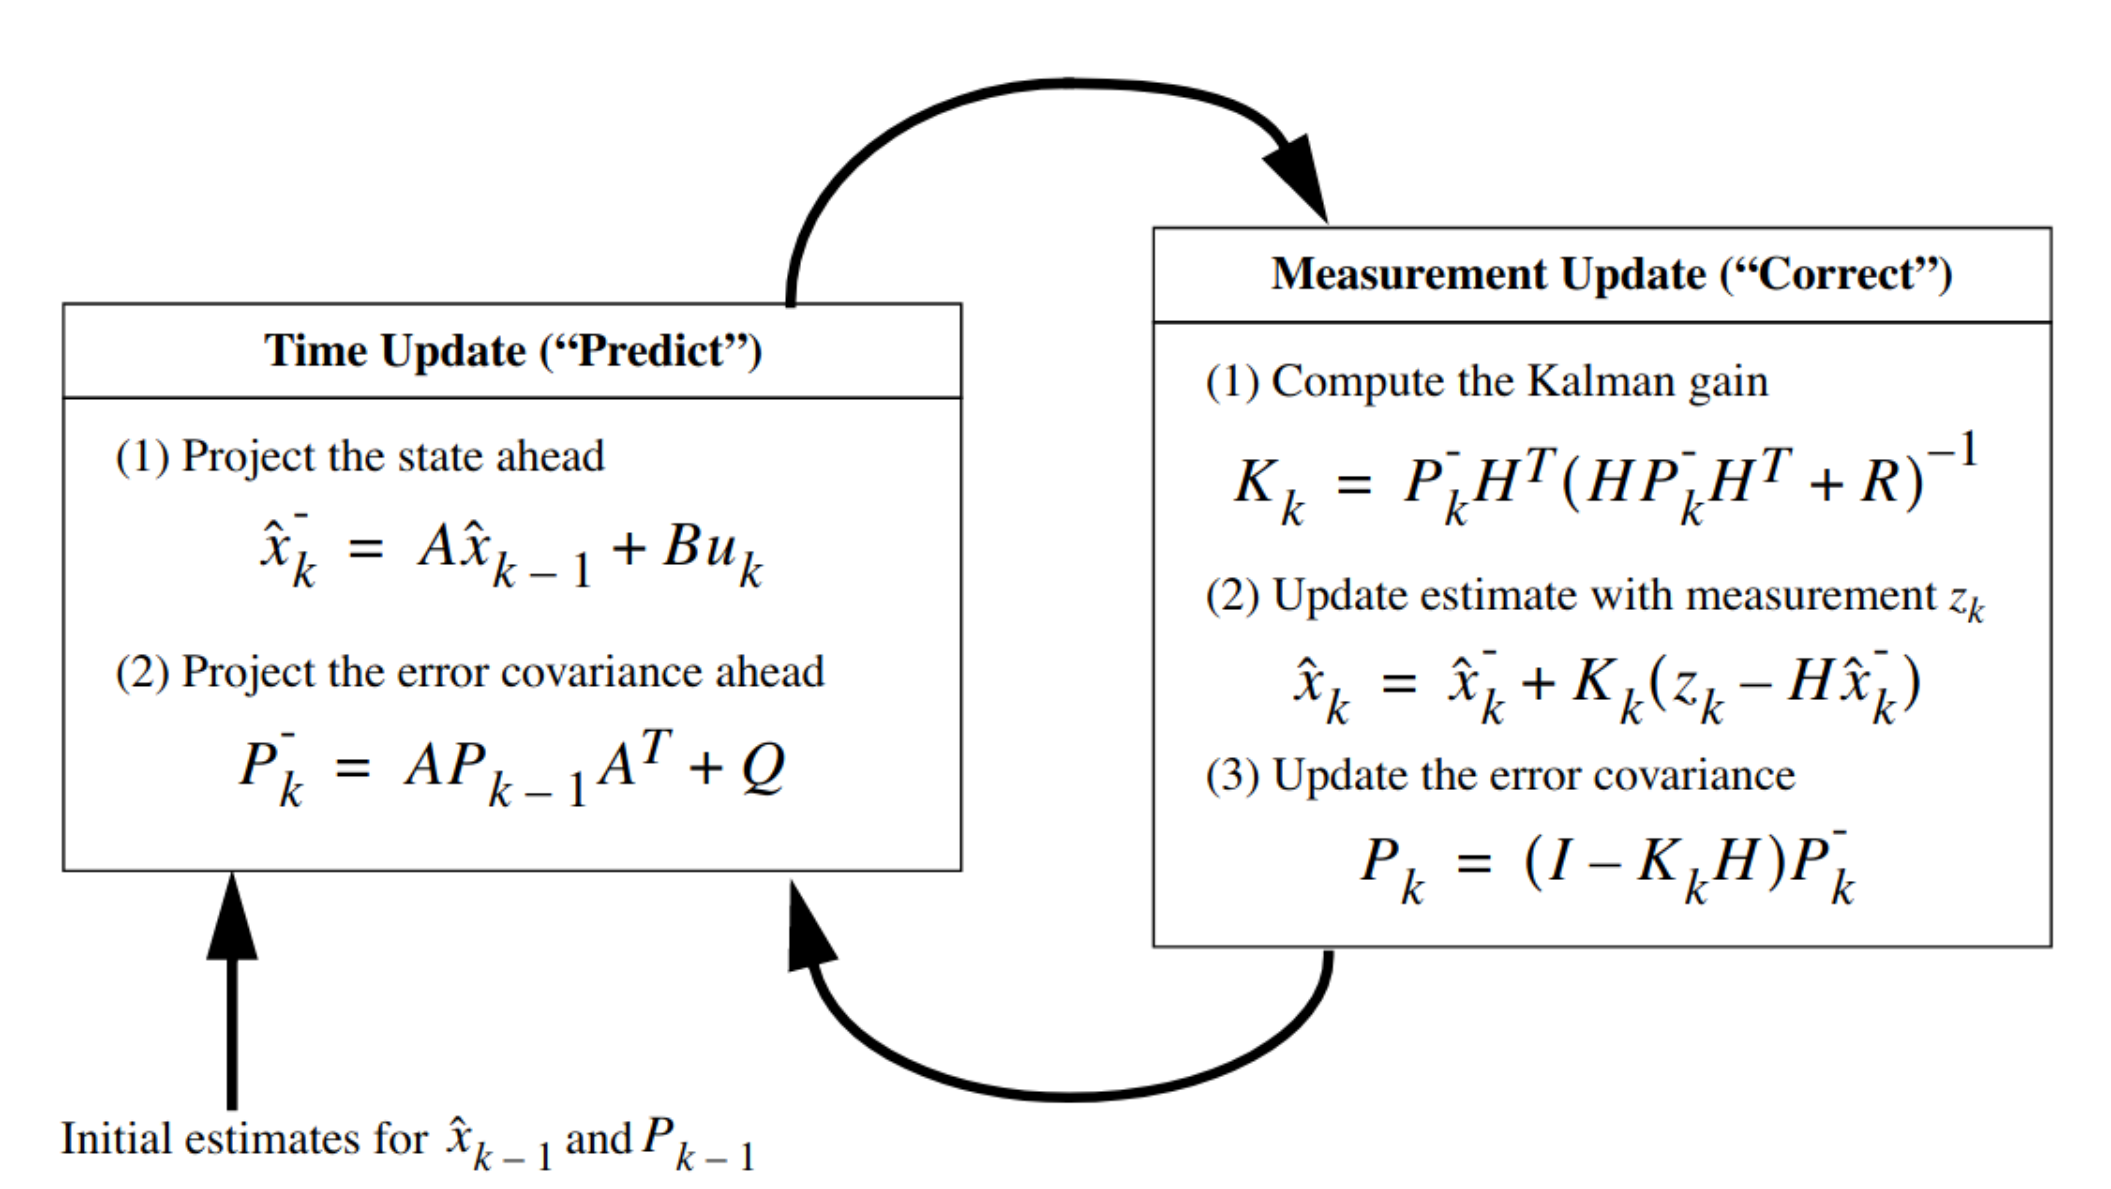
\includegraphics[width=0.7\textwidth]{kf_complete.png}
        \caption{Diagrama detallado del funcionamieno del filtro de Kalman}
        \label{complete_kf}
    \end{center}
\end{figure}

\noindent \'Este m\'etodo puede ser f\'acilmente utilizado para estimar el 
\acrshort{SOC} de una celda. En principio se necesita un modelo linealizado de la 
celda de litio-ion representado en un sistema de ecuaciones de estado e 
implementar el filtro para poder estimar el \acrshort{SOC} tomando una variable 
que se pueda utilizar y medir como salida para poder calcular un error de la 
estimaci\'on del estado, de forma tal que el algoritmo pueda iterar y calcular 
la ganancia de Kalman para poder \emph{corregir} su estimaci\'on.

\noindent Por ejemplo, \emph{Spagnol et. al} propone implementar un filtro de
Kalman utilizando un modelo en ecuaciones de estado que permite fusionar la
representaci\'on de la celda en un modelo el\'ectrico (t\'ipico para
estimaci\'on del \acrshort{OCV}) con metodolog\'ias de conteo de Coulomb
(desarrollada en \ref{ahMethod}) obteniendo un m\'etodo que permite rechazar
tanto el ruido de las mediciones como tambi\'en errores param\'etricos del
modelo.

\noindent Los autores plantean el uso de un modelo el\'ectrico de la bater\'ia
basado en dos tanques RC conectados a una resistencia en serie y dos fuentes de
tensi\'on controladas por el \acrshort{SOC} representa el \acrshort{OCV} de la 
celda, como se puede observar en la Figura \ref{2rc_circuit}.

\newpage

\begin{figure}[h!]
    \begin{center}    
        \begin{circuitikz}[american voltages]
            \draw (0, 0) to[D*] (0, -2);
            \draw (0, -2) to[cV, l=$OCV_{CC}(SoC)$] (0, -4);
            \draw (-1.5, -2) to[D*] (-1.5, 0);
            \draw (-1.5, -2) to[cV, l_=$OCV_{DC}(SoC)$] (-1.5, -4);
            \draw (-1.5, 0) to[short, -*] (0, 0);
            \draw (-1.5, -4) to[short, -*] (0, -4);
            \draw (0, 0) to[R=$R_0$] (2, 0);
            \draw (2, 0) to[short] (2, 1);
            \draw (2, 0) to[short] (2, -1);
            \draw (2, 1) to[R=$R_1$] (4, 1);
            \draw (2, -1) to[C=$C_1$] (4, -1);
            \draw (4, 1) to[short] (4, -1);
            \draw (4, 0) to[short] (5, 0);
            \draw (5, 1) to[short] (5, -1);
            \draw (5, 1) to[R=$R_2$] (7, 1);
            \draw (5, -1) to[C=$C_2$] (7, -1);
            \draw (7, 1) to[short] (7, -1);
            \draw (7, 0) to[short] (8, 0);
            \draw (0, -4) to[short] (8, -4);
            \draw (8, 0)  to[open, v=$v_o$] (8, -4);
        \end{circuitikz}
        \caption{Modelo el\'ectrico utilizado para representar la din\'amica de
        una celda de litio-ion}
        \label{2rc_circuit}
    \end{center}
\end{figure}

\noindent Una vez caracterizado este modelo, se busca obtener un sistema de 
ecuaciones de estado para poder implementar el filtro de Kalman, partiendo desde 
la ecuaci\'on de la tensi\'on de salida sobre un punto conocido del 
\acrshort{SOC} con el objetivo de linealizarlo, una vez planteado este sistema 
de ecuaciones, se puede proceder a implementar el Filtro de Kalman, donde su 
ganancia es recalculada para minimizar el error entre la tensi\'on de salida 
estimada con la obtenida en la medici\'on. 

\noindent Este procedimiento nos permite obtener un algoritmo apto para operar
en tiempo real bajo la aplicaci\'on de un veh\'iculo el\'ectrico, ya que no es
costoso de implementar a nivel de requerimiento computacional y solo depende de
dos sensores, un sensor de corriente y un sensor de tensi\'on que permita medir
ambas variables para fusionarlas dentro del algoritmo. Por \'ultimo, cabe
destacar que el mismo es robusto ante ruido en las mediciones, errores en la
parametrizaci\'on del modelo y error de inicializaci\'on, es decir, tener una
estimaci\'on err\'onea del estado incial del sistema. Esto se puede observar en
los resultados de la Figura \ref{resultados_soc_spagnoli}.

\begin{figure}[h!]
    \begin{center}
        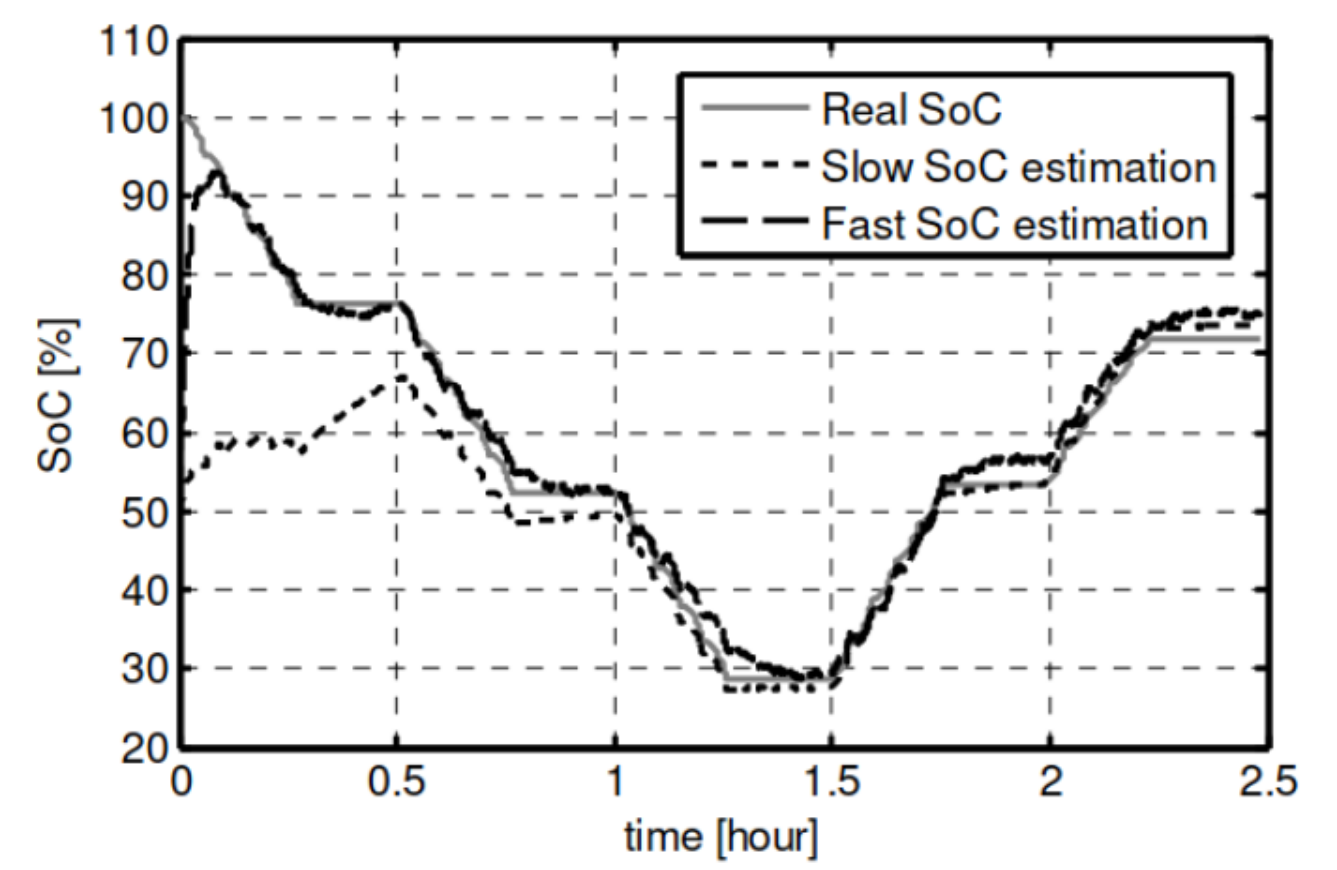
\includegraphics[width=0.7\textwidth]{soc_results_spagnoli.png}
        \caption{Resultados obtenidos en \emph{spagnoli et. al.} sobre la
        estimaci\'on del Kalman con distintos par\'ametros de ajuste, con un
        \acrshort{SOC} inicial de un 50\%, se puede observar que la señal del
        \acrshort{SOC} converge a distintas velocidades al valor real.}
        \label{resultados_soc_spagnoli}
    \end{center}
\end{figure}

\noindent Los resultados de investigaciones relacionadas al Filtro de Kalman
como un observador del Estado de Carga obtuvieron resultados prometedores que
hacen que el algoritmo sea un gran candidato para sistemas en tiempo real, tales
como \acrshort{VVEE} o \acrshort{UPS}.

\subsubsection{M\'etodos basados en el aprendizaje autom\'atico}

\noindent

\newpage


\begin{figure}[h!]
    \begin{subfigure}[b]{.5\textwidth}
	\begin{center}
	    \begin{minipage}[c]{0.45\textwidth}
		\centering
		\begin{circuitikz}[european]

		    \draw (7, 2) -- (7, 2.2);
		    \draw (7, 2) to[battery1] (7, 1.6);
		    \draw (7, 1.4) -- (7, 1.6);
		    \draw (7, 1.4) to[battery1] (7, .9);			
		    \draw (7, .7) -- (7, .9);			
		    \draw (7, 0.7) to[battery1] (7, 0.2);			
		    \draw (7, 0.2) -- (7, -0.2);
		    \draw (7, -0.2) to[battery1] (7, -0.7);
		    \draw (7, -.7) -- (7, -.9);
		    \draw (7, -.9) to[battery1] (7, -1.4);
		    \draw (7, -1.4) -- (7, -1.6);
		    \draw (7, -1.6) to[battery1] (7, -2);
		    \draw (7, -2) -- (7, -2.2);

		    \draw (9, 2) -- (9, 2.2);
		    \draw (9, 2) to[battery1] (9, 1.6);
		    \draw (9, 1.4) -- (9, 1.6);
		    \draw (9, 1.4) to[battery1] (9, .9);			
		    \draw (9, .7) -- (9, .9);			
		    \draw (9, 0.7) to[battery1] (9, 0.2);			
		    \draw (9, 0.2) -- (9, -0.2);
		    \draw (9, -0.2) to[battery1] (9, -0.7);
		    \draw (9, -.7) -- (9, -.9);
		    \draw (9, -.9) to[battery1] (9, -1.4);
		    \draw (9, -1.4) -- (9, -1.6);
		    \draw (9, -1.6) to[battery1] (9, -2);
		    \draw (9, -2) -- (9, -2.2);

		    \draw (11, 2) to[battery1] (11, 1.6);
		    \draw (11, 1.4) -- (11, 1.6);
		    \draw (11, 1.4) to[battery1] (11, .9);			
		    \draw (11, .7) -- (11, .9);			
		    \draw (11, 0.7) to[battery1] (11, 0.2);		
		    \draw (11, 0.2) -- (11, -0.2);
		    \draw (11, -0.2) to[battery1] (11, -0.7);
		    \draw (11, -.7) -- (11, -.9);
		    \draw (11, -.9) to[battery1] (11, -1.4);
		    \draw (11, -1.4) -- (11, -1.6);
		    \draw (11, -1.6) to[battery1] (11, -2);
		    \draw (11, -2) -- (11, -2.2);

		    \draw (7, 0) -- (9, 0);
		    \draw (9, 0) -- (11, 0);

		    \draw (7, 0.8) -- (9, 0.8);
		    \draw (9, 0.8) -- (11, 0.8);

		    \draw (7, 1.5) -- (9, 1.5);
		    \draw (9, 1.5) -- (11, 1.5);

		    \draw (7, 2.2) -- (9, 2.2);
		    \draw (9, 2.2) -- (11, 2.2);			

		    \draw (7, -0.8) -- (9, -0.8);
		    \draw (9, -0.8) -- (11, -0.8);

		    \draw (7, -1.5) -- (9, -1.5);
		    \draw (9, -1.5) -- (11, -1.5);

		    \draw (7, -2.2) -- (9, -2.2);
		    \draw (9, -2.2) -- (11, -2.2);			

		    \draw [dashed] (6.5, 2.4) rectangle (11.5, -2.4);

		    \draw node at (8.2, 2.6) {Pack de Baterías 6s3p};
		\end{circuitikz}
	    \end{minipage}
	\end{center}
	\caption{Esquemático de la arquitectura del pack de baterías.}
	\label{pack_bateria}
    \end{subfigure}%
    ~
    \begin{subfigure}[b]{.45\textwidth}
	\centering
	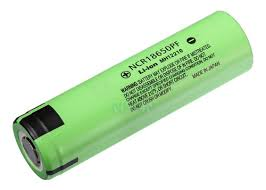
\includegraphics[width=0.7\textwidth]{18650.jpg}
	\caption{Foto celda NCR18650PF.}
	\label{foto_bateria}
    \end{subfigure}
    \caption{Pack 6s3p y Celda NCR18650PF.}
    \label{pack}
\end{figure}
\FloatBarrier

Estas celdas se caracterizan por su cátodo, cuya composición química se basa en
el óxido de litio niquel cobalto aluminio ($\mathrm{LiNiCoAlO_2}$) y, según su
hoja de datos \cite{18650_datasheet}, sus carateristicas electricas se pueden
observar en la Tabla \ref{table:ncr}. 

\begin{table}[h]
    \begin{center}
	\begin{tabular}{|c|l|}
	    \hline
	    \multicolumn{2}{|c|}{Especificaciones el\'ectricas}                          \\ \hline
	    \textbf{Capacidad Específica}                 & 2700mAh                            \\ \hline
	    \multirow{2}{*}{\textbf{Capacidad}}           & Mínimo: 2750mAh                    \\ \cline{2-2} 
	    & Tipico: 2900mAh                    \\ \hline
	    \textbf{Corriente de Descarga Máxima}         & 10000mAh($\sim$3.5C)               \\ \hline
	    \textbf{Rango operativo de tensión}           & 2.5V - 4.2V                        \\ \hline
	    \textbf{Voltaje Nominal}                      & 3.6V                               \\ \hline
	    \textbf{Charga}                               & CC-CV, Std. 1375mA, 4.20V, 4.0 hrs \\ \hline
	    \textbf{Peso}                                 & 48g                              \\ \hline
	    \multirow{3}{*}{\textbf{Temperatura}}         & Carga: 0 a 45C                     \\ \cline{2-2} 
	    & Descarga: -20 a 60C                \\ \cline{2-2} 
	    & Almacenaje: -20 a 50C              \\ \hline
	    \multirow{2}{*}{\textbf{Densidad Energética}} & Volum\'etrica: 577Wh/l               \\ \cline{2-2} 
	    & Gravim\'etrica: 207wh/kg             \\ \hline
	\end{tabular}%
	\caption{Especificaciones el\'ectricas de una celda de litio NCR18650PF}
	\label{ncr_table}
    \end{center}
\end{table}

Por el otro lado, la hoja de datos también nos provee curvas significativas,
como por ejemplo, la curva de carga \emph{(Fig. \ref{cc_cv_18650})}, la curva de
descarga para distintas corrientes \emph{(Fig. \ref{descarga_18650})} y la curva
del ciclo de vida típico de la batería \emph{(Fig. \ref{life_cycle_18650})}.

\begin{figure}[h!]
    \begin{subfigure}[t]{.5\textwidth}
	%   		\centering
	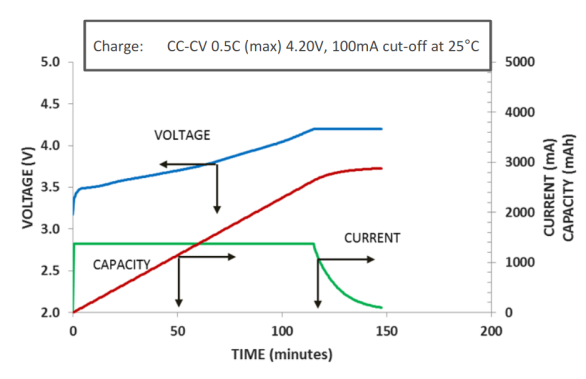
\includegraphics[width=0.9\textwidth]{cc_cv_18650.png}
	\caption{Curva de carga.}
	\label{cc_cv_18650}
    \end{subfigure}%
    ~ 
    \begin{subfigure}[t]{.5\textwidth}
	%    		\centering
	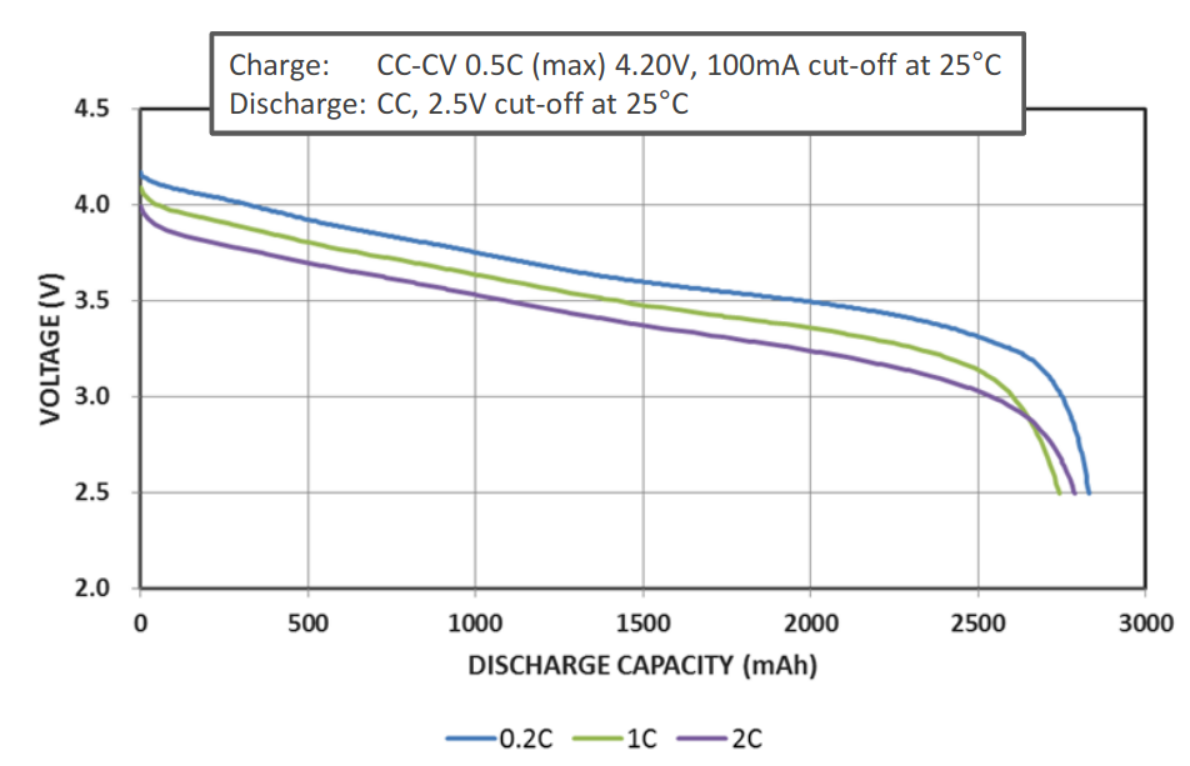
\includegraphics[width=0.9\textwidth]{discharge_18650.png}
	\caption{Curva de descarga en base a distintas corrientes de descarga (0.5C,
	1C, 1.5C y 2C)}
	\label{descarga_18650}
    \end{subfigure}
    ~ 
    \begin{centering}
	\begin{subfigure}[t]{1\textwidth}
	    \centering
	    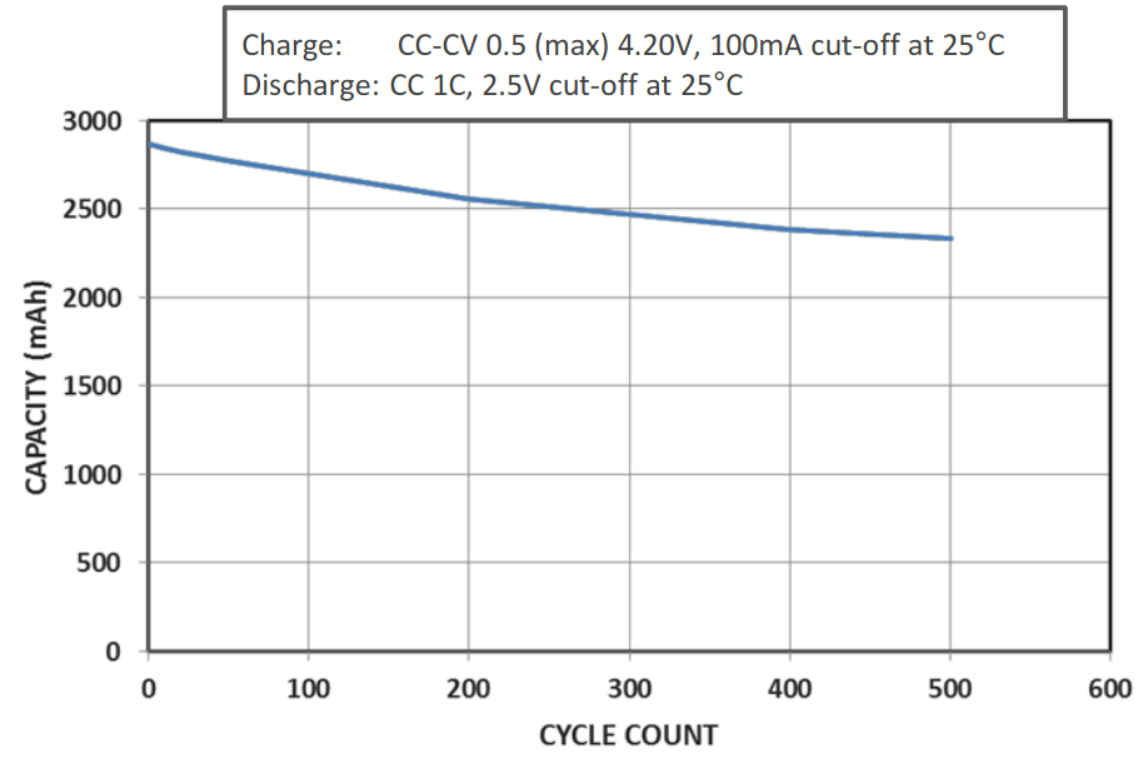
\includegraphics[width=0.4\textwidth]{life_cycle_18650.png}
	    \caption{Curva del ciclo de vida de una celda 18650}
        \label{life_cycle_18650}
	\end{subfigure}
    \end{centering}
    \caption{Curvas sgnificativas celda Panasonic 18650PF}
    \label{curvas_sign_18650}
\end{figure}

\newpage 

\subsection{Sensado de Corriente}

El sensado de la corriente de carga como de descarga del pack de batería juega
un rol muy importante en el desarrollo exitoso de un \acrshort{BMS}. Es a partir
de conocer con precisión la magnitud de corriente que el sistema podrá mantener
el pack de baterías operando dentro de la zona segura (\acrshort{SOA} por sus
siglas en ingles), monitorear la distribución de carga entre las celdas,
implementar correctamente los algoritmos de ecualización de carga y mantener un
seguimiento preciso del estado de carga.

\noindent Existen en el mercado una gran variedad de tecnologías y 
soluciones para la medición de corriente en las diferentes aplicaciones. 
Algunas de las tecnologías mas relevantes, disponibles en el mercado son:
\begin{itemize}
    \item Resistencia Shunt
    \item Transformadores de intensidad (TI)
    \item Bobina de Rogowski 
    \item Sensores de Efecto Hall
    \item Sensores de Impedancia Magnética (MI)
    \item Sensores de Magnetoresistencia Gigante 
    \item Sensores Ópticos (Experimental)
\end{itemize}

Dentro del amplio abanico de métodos y tecnologías utilizadas para la medición
de corrientes los dos más elegidos e implementados en Sistemas de Administración
de Baterías \acrshort{BMS} son las mediciones a partir de resistencias Shunt y
mediciones a partir de sensores de efecto hall.

\subsubsection{Resistencia Shunt}

La tecnología Shunt se vale del Sensado de la caída del voltaje sobre una
resistencia de unos pocos mili ohmios en serie con el paso de la corriente
incógnita para la medición indirecta de la corriente.

El método de sensado por resistencia tipo shunt presenta una de las mejores
relaciones costos-efectividad, presentando un empaquetado compacto y aplicable
en mediciones de corrientes tanto continua como alterna encontrando su
frecuencia de corte por encima de las decenas de Mhz.

Las mediciones por resistencia shunt carecen naturalmente de aislación galvánica
debiendo ser resuelta a partir del circuito de implementación. Generalmente, los
shunts presentan bajo coeficiente de temperatura de resistencia, (\acrfull{TCR}
por sus siglas en ingles). Característica fundamental en las implementaciones de
\acrshort{BMS} en sistemas de vehículos eléctricos que permite aumentar el rango
de temperatura de operación del sistema.

Aunque los shunts de corrientes operen bajo el principio de caida de voltaje
ohmico, en la práctica las resistencias presentan una inductancia intrínseca que
comprometen la precisión y el ancho de banda máximo de las mediciones.

\subsubsection{Sensor de efecto Hall}

El sensor de efecto Hall es un sensor de efecto magnético basado en el fenómeno
físico homónimo que le da su nombre.  El sensor de efecto Hall es un dispositivo
aislado, no intrusivo que puede ser utilizado para medir corriente tanto
continua como alterna de hasta unos cientos de kHz. El sensor Hall puede ser
fabricado utilizando tecnología CMOS convencional pero a un costo mayor que las
implementaciones con transformadores de corriente o bobinas de Rogowski.

El traductor de efecto Hall encuentra normalmente su límite de medición en los
picos de corriente debido al fenómeno de saturación magnética del núcleo y
encuentra su límite de ancho de banda en las frecuencias menores al MHz. A su
vez, esta tecnología es sumamente sensible a la influencia de los campos
magnéticos externos. Frente a estas limitaciones es común que los sensores de
efecto Hall se implementen mayoritariamente con bobinas cerradas para lograr una
mejor precisión y un rango mayor de operación dinámico.

El voltaje de offset presente en la medición del dispositivo es poco estable y
varia fuertemente frente a las variaciones de temperatura de operación.

\begin{figure}[h!]
    \centering
    \begin{subfigure}[b]{0.4\linewidth}
	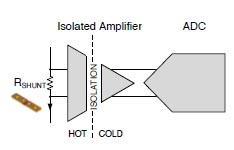
\includegraphics[width=\linewidth]{../assets/R-Shunt_Isolated_Sensor.jpg}
	\caption{Sensado por Resistencia Shunt}
    \end{subfigure}%
    \hspace{15mm}
    \begin{subfigure}[b]{0.4\linewidth}
	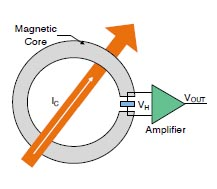
\includegraphics[width=\linewidth]{../assets/Open-loop_Hall_Sensor.jpg}
	\caption{Sensado por efecto Hall de loop abierto}
    \end{subfigure}
    \caption{Diagramas - Métodos de sensado de corriente}
    \label{fig:SenseMetods}
\end{figure}

\subsubsection{Tecnología Seleccionada}

Frente a los requerimientos y la naturaleza de un \acrshort{BMS} hemos
seleccionado la tecnología de sensado de corriente por resistencia Shunt.
Actualmente existen en el mercado un sin número de soluciones de amplificadores
y moduladores aislados que permiten alcanzar precisas mediciones de corrientes
con este método logrando minimizar las injerencias del entorno siempre y cuando
se seleccione una resistencia Shunt adecuada.

\noindent Las ventajas de la medición a partir del método de resistencia 
shunt son:

\begin{itemize}
    \item Bajo offset y baja susceptibilidad frente a influencias de campos 
	magnéticos externos y variaciones de temperatura.
    \item Alta linealidad de la solución en todo el rango de voltaje en 
	comparación a la solución basada en tecnología Hall, sobre todo en 
	la zona cercana a cero y la de saturación del nucleo. 
    \item Mejor resolución para mediciones de corriente continua frente a 
	las soluciones basadas en mediciones de efecto Hall. 
	Particularmente debido a la baja sensitividad que presenta frente a 
	las influencias de los campos magnéticos externos.
    \item Pueden soportar operaciones en ambientes de altas temperaturas 
	manteniendo la linealidad debido a su bajo TCR. 
	Los sensores de efecto Hall encuentran su rango de operación 
	fuertemente acotado.
    \item Facilidad que presenta la tecnología para la integración en 
	circuitos impresos priorizando el tamaño reducido.
    \item Disponibilidad en distribuidores nacionales
\end{itemize}

\noindent El integrado propuesto para el sensado de corriente es el INA226 de
Texas Instruments. El INA226 es un conversor analógico digital de 16 bits (ADC)
que implementa una interfaz compatible I2C para la comunicación con el módulo
del control. El dispositivo monitorea simultaneamente la tensión que cae en una
resistencia shunt y la del bus de alimentación. Permite múltiples calibraciones
y seteos, entre ellos variar los tiempos de conversión y definir conversiones
múltiples que al implementar internamente un multiplicador y divisor permite
obtener lecturas directas de tensión y potencia en amperes y en Vatios.

Observamos en la figura \ref{fig:ina226-commonimplementation} su implementación
modelo. 

\begin{figure}[h!]
    \begin{center}
	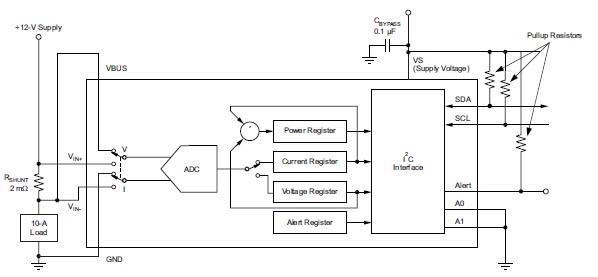
\includegraphics[width=0.7\linewidth]{assets/INA226-Common_Implementation}
	\caption{Implementación Tipo - INA226}
	\label{fig:ina226-commonimplementation}
    \end{center}	
\end{figure}
\FloatBarrier

\subsection{Simulaciones}

\subsubsection{Simulación Filtro de Kalman}

Para la implementación de este filtro es necesario obtener un modelo en espacio
de estados de la batería de la forma :

\begin{align}
    \dot{x}(t) = Ax+Bu	\nonumber\\
    y(t)=Cx+Du
    \label{SS_Model_generic}	
\end{align}

Para tal fin tomamos como referencia un modelo eléctrico con 2 elementes RC en
serie, también conocido como modelo de Randles de segundo orden, representado en
la figura \ref{Randles_2do}, ya que este módelo tiene amplia aceptación debido a
que ofrece un grado de ajuste alto sin resultar en un excesivo costo
computacional en comparación con modelos electroquímicos de la batería.

\begin{figure}[h!]
    \begin{center}
	\begin{minipage}[c]{0.95\textwidth}
	    \centering
	    \ctikzset{bipoles/length=1.0cm}
	    \ctikzset{bipoles/resistor/height=.3}

	    \begin{circuitikz}[american]

		\draw (0,0) to[R=$R_0$] (3,0) -- (3,-0.5) to[R=$R_1$] (6,-0.5) -- (6,0);
		\draw (3,0) -- (3,0.5) to[C=$C_1$,v=$ $] (6,0.5) -- (6,0);
		\draw (6,0) to[short,-*] (6.5,0) -- (7,0) -- (7,0.5) to[C=$C_2$,v=$ $] (10,0.5) to[short,-o] (10,0);
		\draw (7,0) -- (7,-0.5) to[R=$R_2$] (10,-0.5) -- (10,0) to[short,f=$i$] (11.5,0);
		\draw  (0,0) to[battery2=$OCV(SOC)$] (0,-3) -- (11.5,-3); 
		\draw  (11.5,0) to [open,v=$v$,invert] (11.5,-3);
		\draw (8.5,1.75) node[anchor=north]{$V_{C2}$};
		\draw (4.5,1.75) node[anchor=north]{$V_{C1}$};
	    \end{circuitikz}
	\end{minipage}
    \end{center}
    \caption{Circuito de Randles de Segundo Orden.}
    \label{Randles_2do}
\end{figure}
\FloatBarrier

\noindent La fuente de tensión controlada $OCV(SoC)$ es linealizada para 
obtener un modelo lineal de la batería e ignoramos el hecho de la histéresis 
respecto a la carga y a la descarga.

Obteniendo una ecuación lineal de la forma \ref{SOC_linearized}, cuyos
parametros fueron obtenidos mediante la función \emph{polyfit} de matlab como se
muetra en la figura \ref{SOC_vs_OCV}.

\begin{equation}
    OCV = SOC \times K_e + OCV_0
    \label{SOC_linearized}
\end{equation}

\begin{figure}[h!]
    \begin{center}
	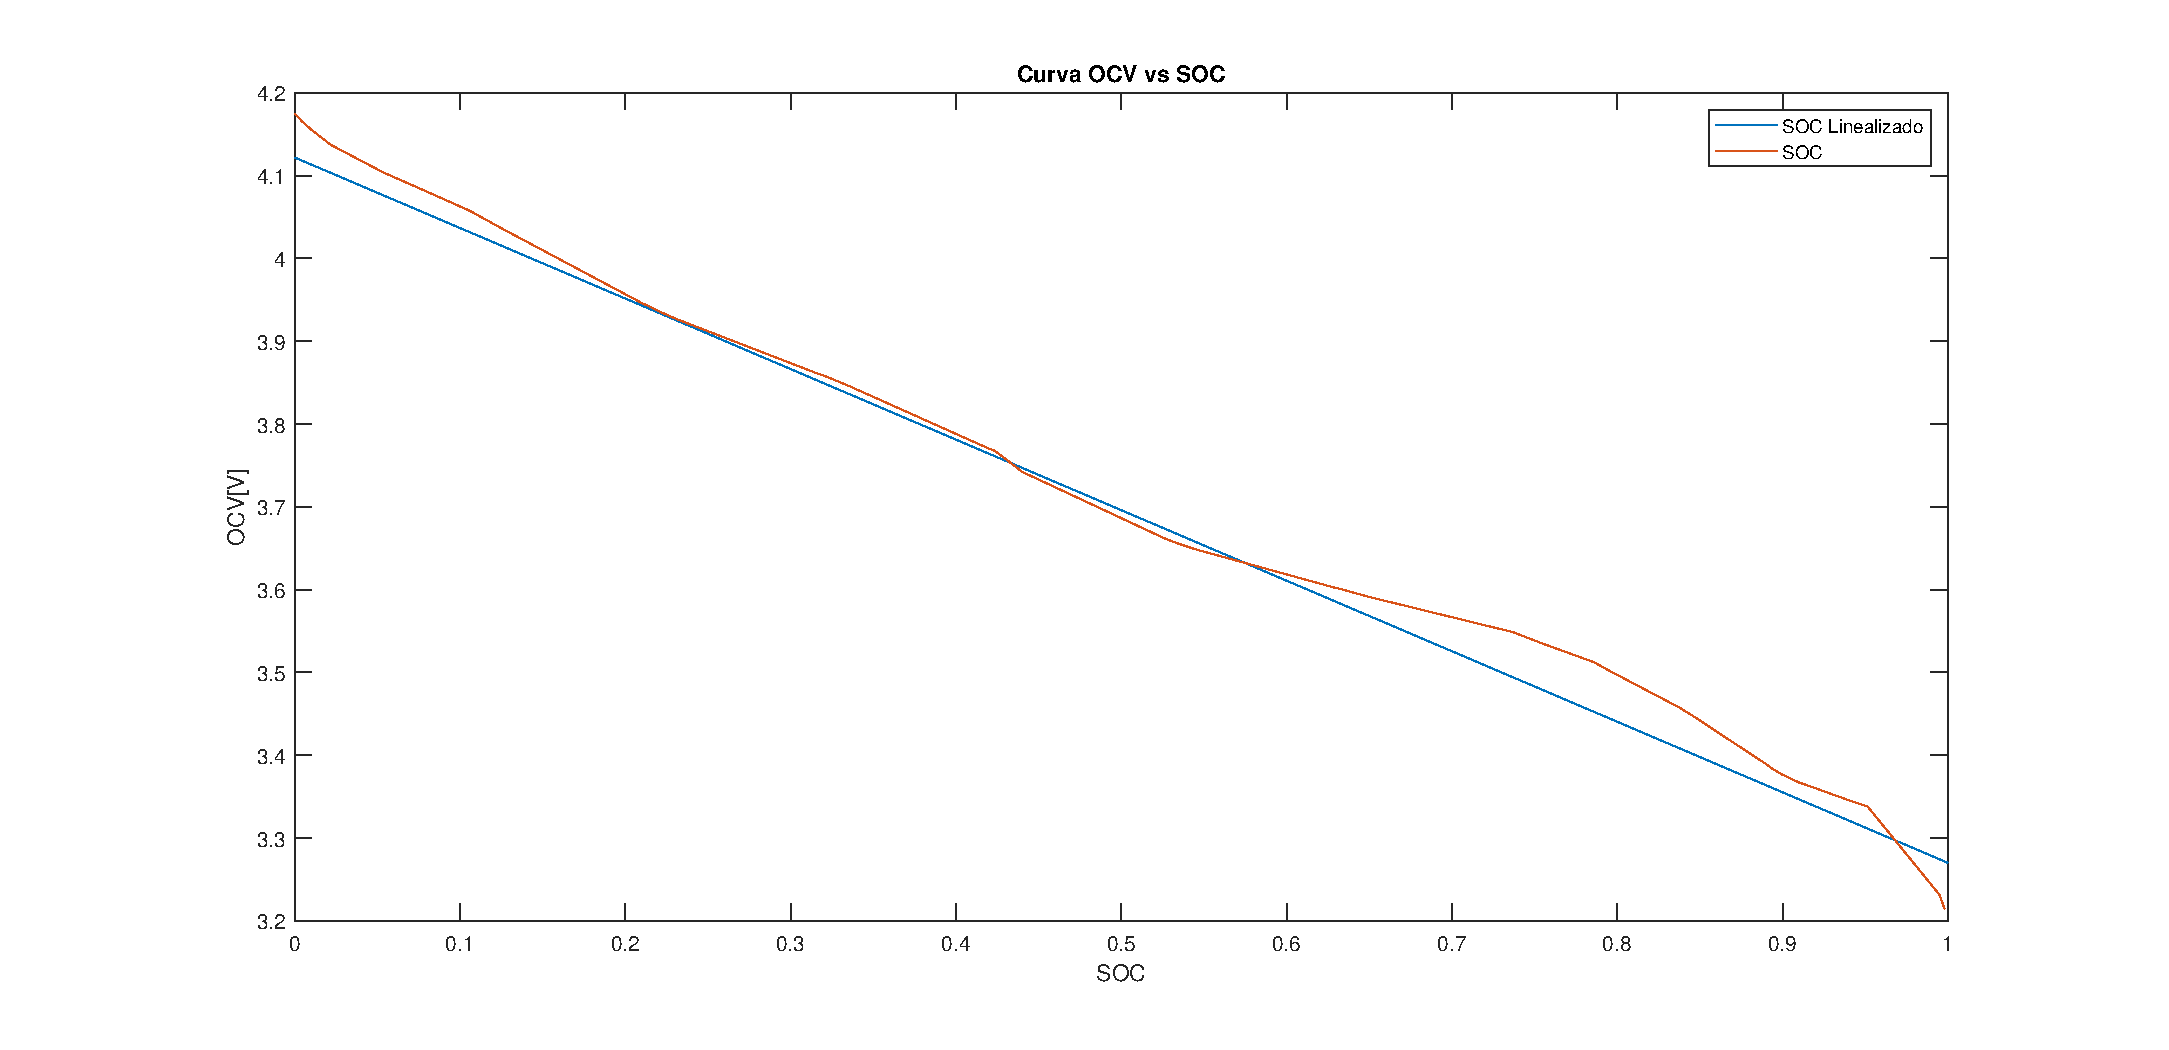
\includegraphics[width=1\textwidth]{SOC_vs_OCV.eps}
	\caption{Curva de SOC vs OCV con su correspondiente linealización }
	\label{SOC_vs_OCV}
    \end{center}
\end{figure}
\FloatBarrier

Nuestro modelo eléctrico tiene 2 grados de libertad y se agrega una 3° variable
de estado que es el estado de carga de la batería. Luego tomando la expresión
diferencial de la ecuación \ref{SOC_Coulomb_C}, seleccionando arbitrariamente
las tensiones en $C_1$ y $C_2$, y tomando como entrada del sistema la corriente
de la batería y como salida la tensión en bornes de la misma obtenemos el
siguiente conjunto de ecuaciones \ref{SS_model_eq}.

\begin{equation}
    \begin{array}{llcllcl}
	\dot{x} & = & \begin{bmatrix}
	    -\frac{1}{R_1 C_1} &            0       & 0 \\
	    0                  & -\frac{1}{R_2 C_2} & 0 \\
	    0                  &            0       & 0 \\
	\end{bmatrix} & x & + &     \begin{bmatrix}
	    -\frac{1}{C_1} \\
	    -\frac{1}{C_2}  \\
	    -\frac{1}{3600 S_{C,a}}\\
	\end{bmatrix} & i \\
	\\
	y & = & \begin{bmatrix}
	    -1-1-K_e 
	\end{bmatrix} & x & + & \begin{bmatrix}
	    R_0
	\end{bmatrix} & i \\
    \end{array}
	\label{SS_model_eq}
\end{equation}

Donde $S_{C,a}$ es la Capacidad Nominal en Ah de la batería. 

Para hacer un ajuste de parámetros de las baterías se utilizó un dataset
provisto por la universidad de Winsconsin-Madison por el Dr. Phillip Kollmeyer
\cite{Kollmeyer2018}. si bien todos los parámetros son dependientes del estado
de carga, seleccionamos los correspondientes al 90\%, ya que las variaciones mas
fuertes de los mismos se dan al entre el 0-10\% y en valores cercanos al 100\%

\begin{figure}[h!]
    \begin{center}
	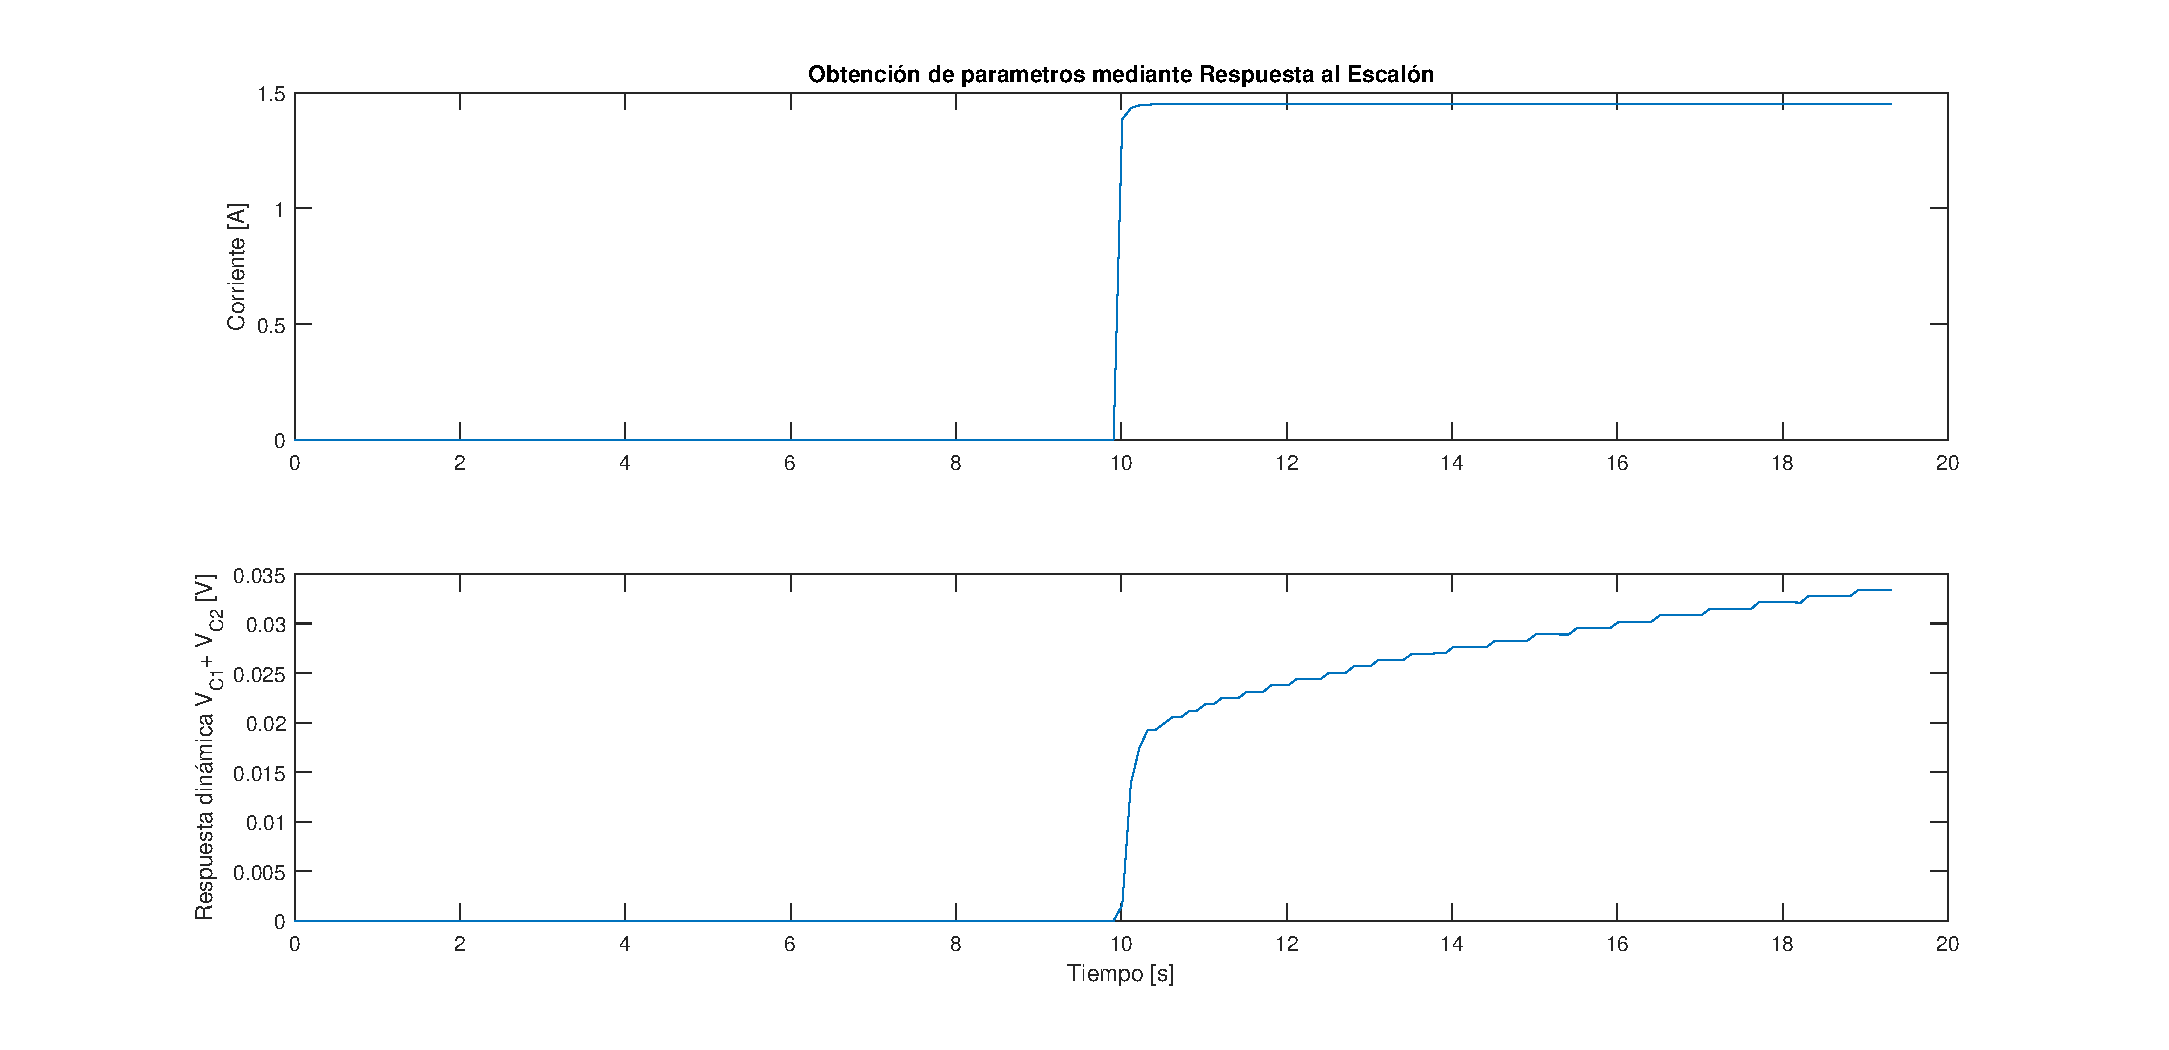
\includegraphics[width=0.85\textwidth]{rta_escalon.eps}
	\caption{Estudio de la Rta al escalón para estimación de parámetros}
	\label{rta_escalon}
    \end{center}
\end{figure}
\FloatBarrier

También se necesita proporcionar valores de Varianza del modelo, ruido al que
están sometidas las variables medibles, el estado inicial estimado y la varianza
de esta estimación estas son denominadas Q,R,$x_0$ y $P_0$ respectivamente.

\noindent Partiendo de la base que nuestro sistema debe ser robusto ante la mala
estimación inicial del estado de carga vamos a proponer un vector de estimación
de estado inicial con un SoC con un error de 80\%.

\begin{equation}
    \begin{array}{llll}
	P_0 & = & \begin{bmatrix}
	    1 & 0 & 0 \\
	    0 & 1 & 0 \\
	    0 & 0 & 1 \\
	\end{bmatrix} 
    \end{array} \nonumber
\end{equation}

\noindent El ciclo de la bateria esseleccionado comienza con la batería cargada
al 100\%, por lo que un error del 80\% se corresponde con 0.2 en el estado de
carga relativo.

\begin{equation}
    \begin{array}{llll}
	x_0 & = & \begin{bmatrix}
	    0 \\
	    0 \\
	    0.2 \\
	\end{bmatrix} 
    \end{array} \nonumber
\end{equation}

\noindent El error en nuestra observación es del orden de los milivoltios
(mV) calculado en base a la resolución del sensor.

\begin{equation}
    R = 0.01  \nonumber
\end{equation}

\noindent El error en nuestro modelo se estima bajo ya que los dataset nos 
proveen una buena fuente de información obtenida en base a ensayos de 
laboratorio

\begin{equation}
    \begin{array}{llll}
	Q & = & \begin{bmatrix}
	    1\cdot10^{-6} & 0 & 0 \\
	    0 & 1\cdot10^{-6} & 0 \\
	    0 & 0 & 1\cdot10^{-6} \\
	\end{bmatrix} 
    \end{array} \nonumber
\end{equation}

Por último se volcaron estos parámetros en un bloque de la librería \emph{System
Identification Toolbox} que corre el algoritmo del filtor de Kalman. Además se
simuló en paralelo el circuito eléctrico equivalente, como se observa en la
Figura \ref{simulink_diagram}.

\begin{figure}[h!]
    \begin{center}
	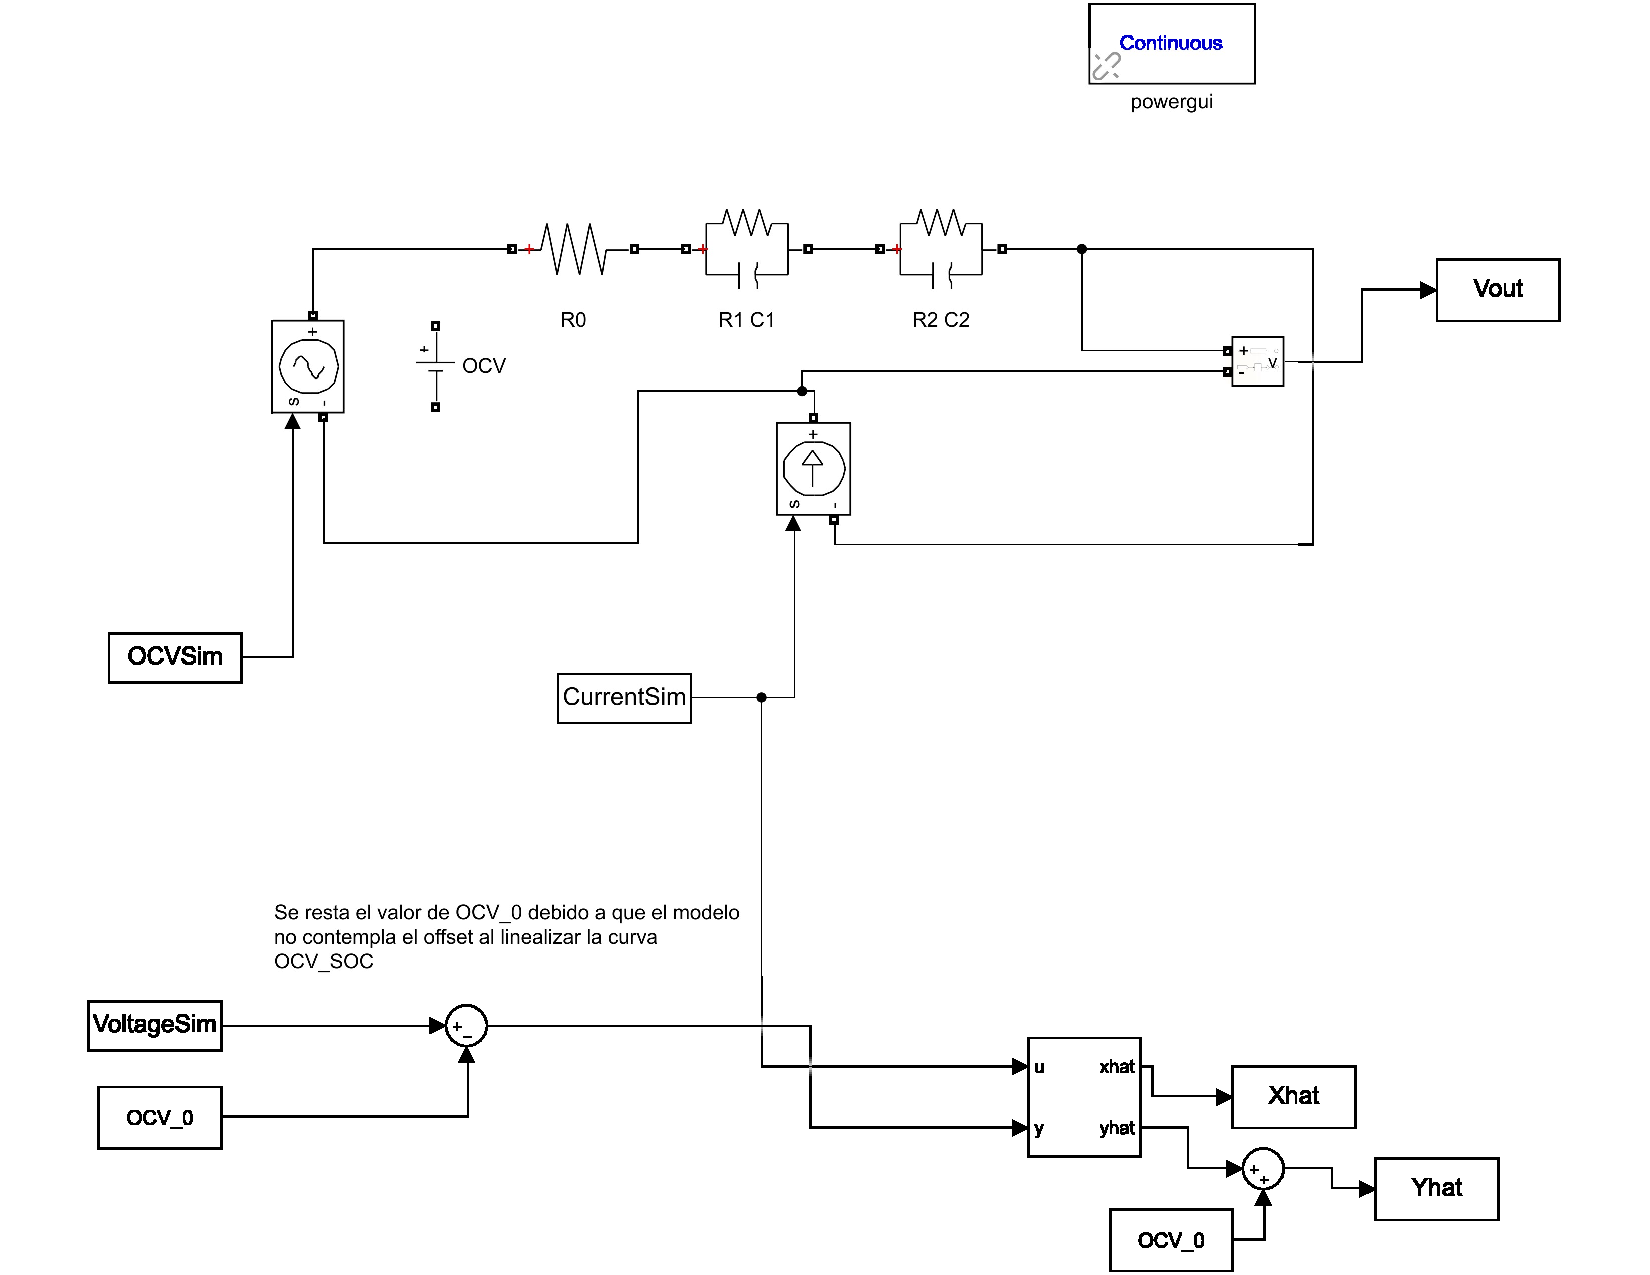
\includegraphics[width=0.95\textwidth]{simulink.pdf}
	\caption{Diagrama de Simulink utilizado para simular el Filtro de Kalman}
	\label{simulink_diagram}
    \end{center}
\end{figure}

Los resultados de la simulación se muestran a continuación en las Figuras
\ref{Tension_sim} y \ref{Tension_sim_zoom} correspondientes a la tensión en
bornes de la batería y  a las Figuras \ref{Drive_Cycle_1_SOC_sim} y
\ref{error_SOC_Sim}, las cuales corresponden al SOC simulado y a un contraste
del error tomando como valor verdadero el SOC provisto por el dataset.

\begin{figure}[h!]
    \begin{center}
	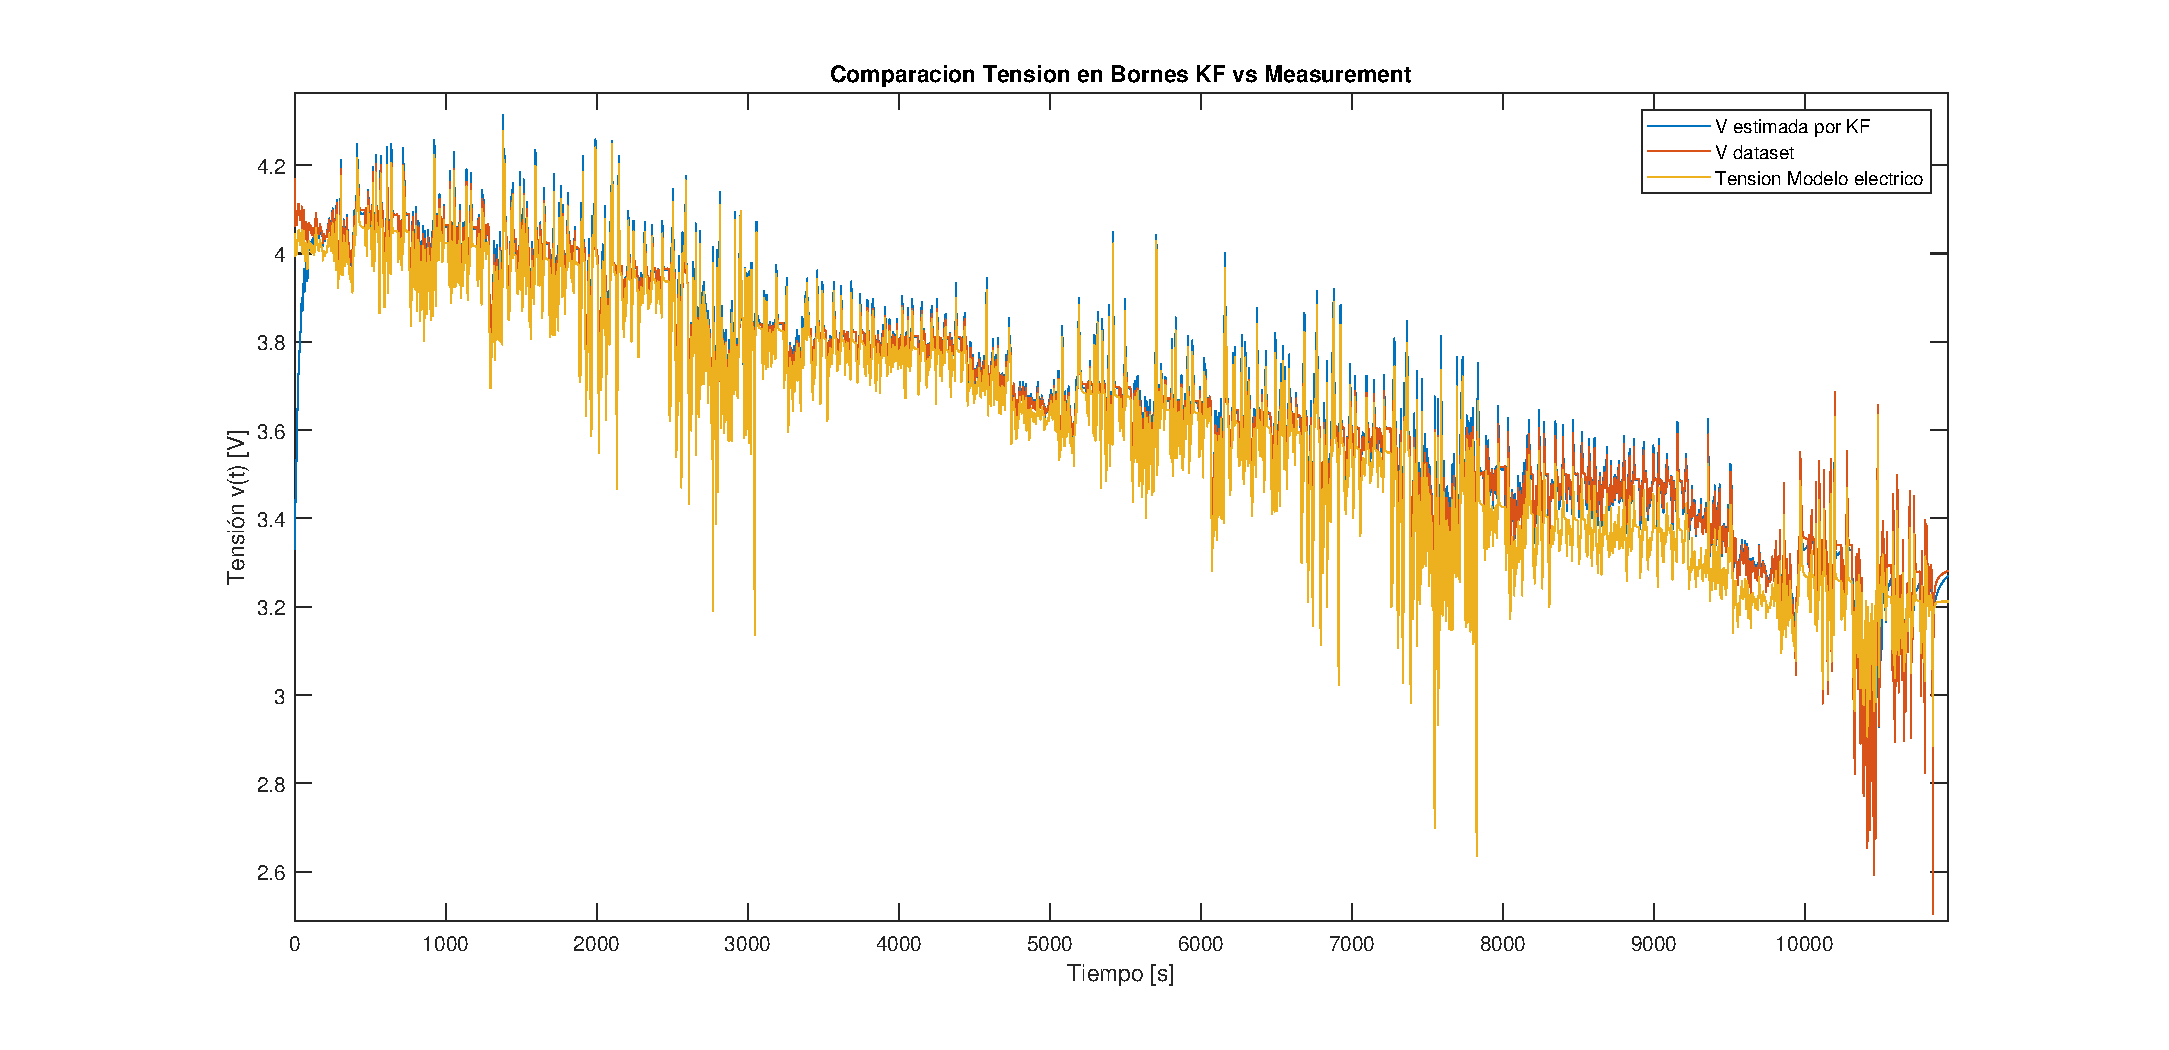
\includegraphics[width=1\textwidth]{Tension_Sim.eps}
	\caption{Resultado de la Simulación de la tensión en bornes de la 
	batería sometida a condiciones de ciclo de manejo}
	\label{Tension_sim}
    \end{center}
\end{figure}

\begin{figure}[h!]
    \begin{center}
	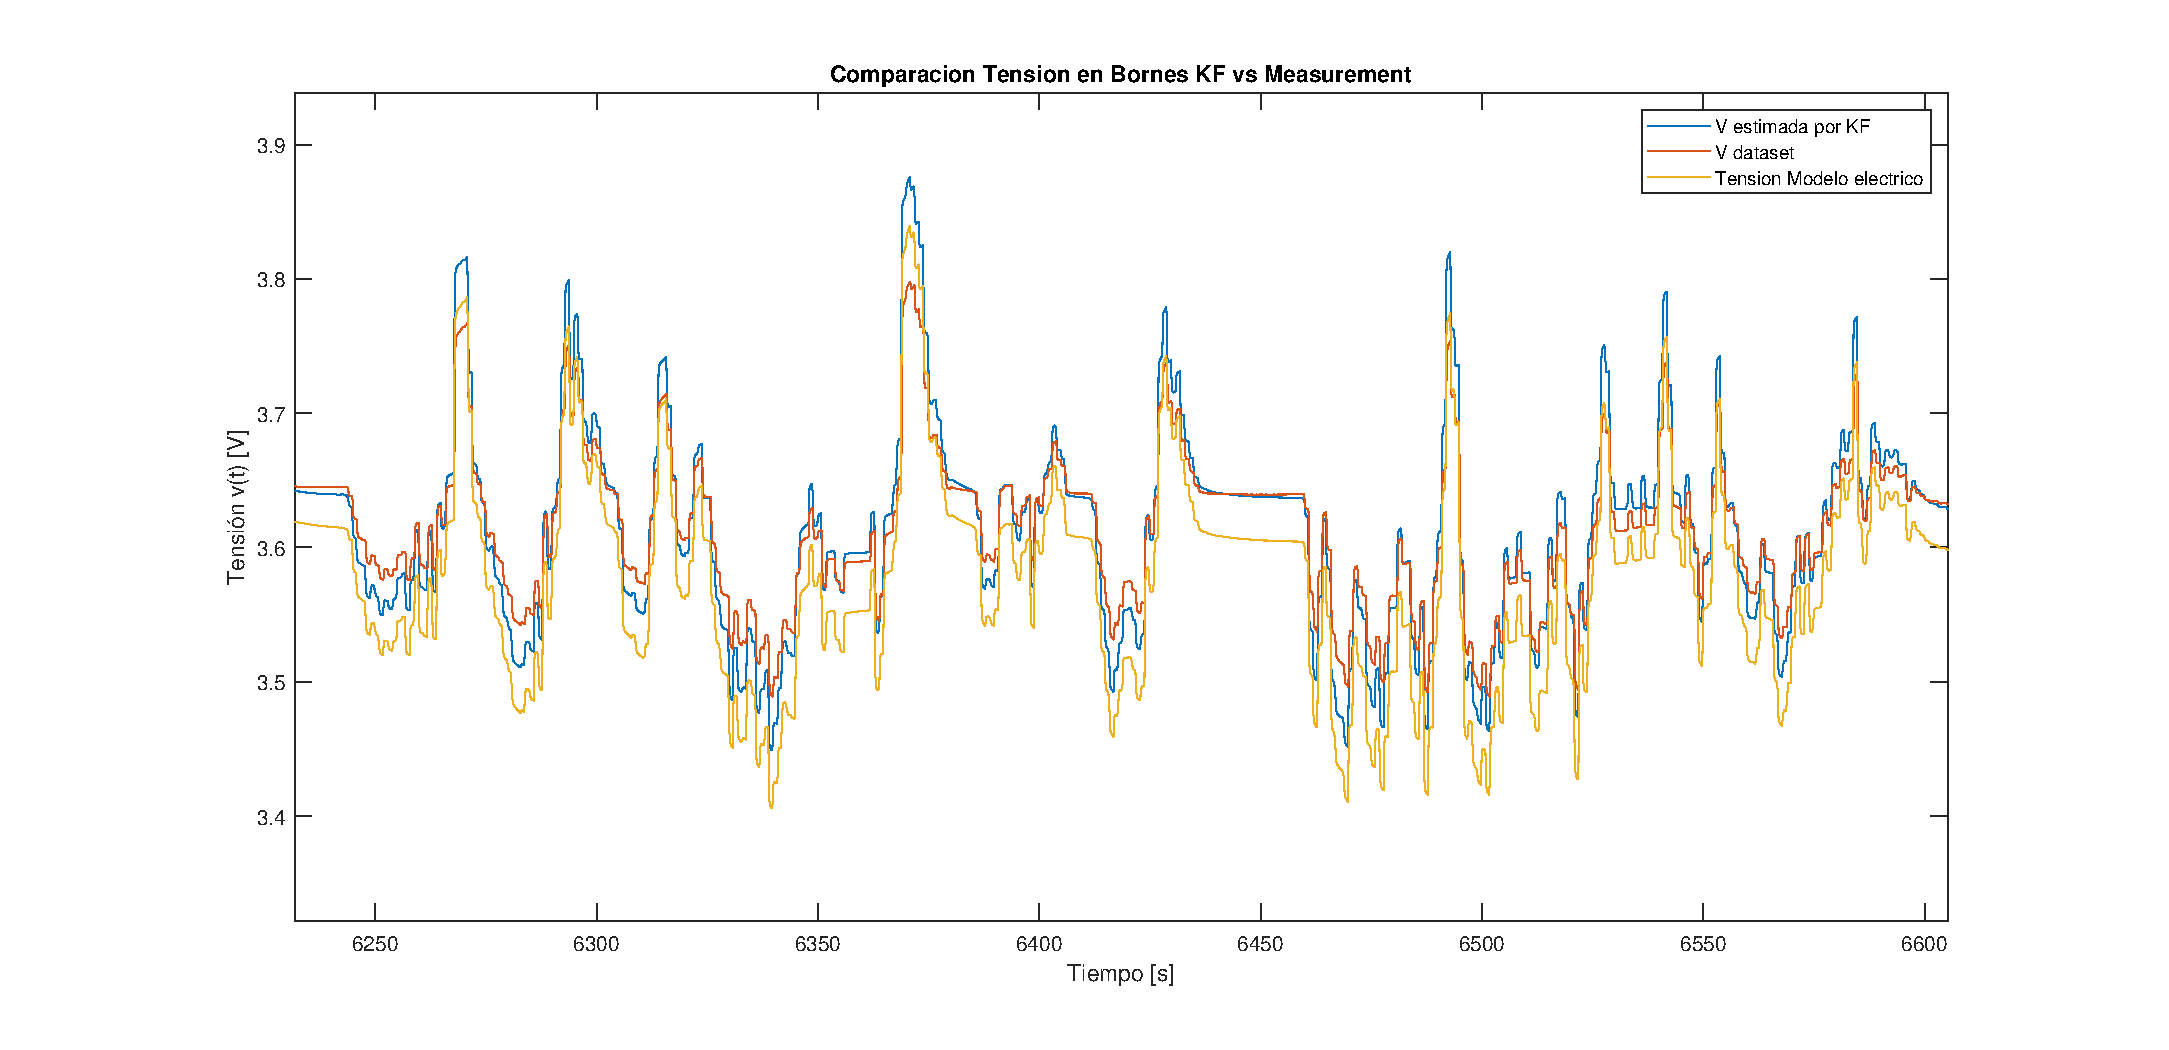
\includegraphics[width=0.95\textwidth]{Tension_Sim_zoom.eps}
	\caption{Detalle de la Simulación de la tensión en bornes de la batería
	sometida a condiciones de ciclo de manejo}
	\label{Tension_sim_zoom}
    \end{center}
\end{figure}

Si se presta especial atención el error se mantiene en una cota del 6 \% hasta
que se dispara en la región de SOC menor al 15\% donde el sistema se vuelve
fuertemente alineal y nuestro modelo pierde validéz. Por otro lado cumple
satisfactoriamente con la corrección del SOC inicial ya que estaba seteado en 20
\% y el Filtro corrige rapidamente a un valor aproximado de 100 \%. 

\begin{figure}[h!]
    \begin{center}
	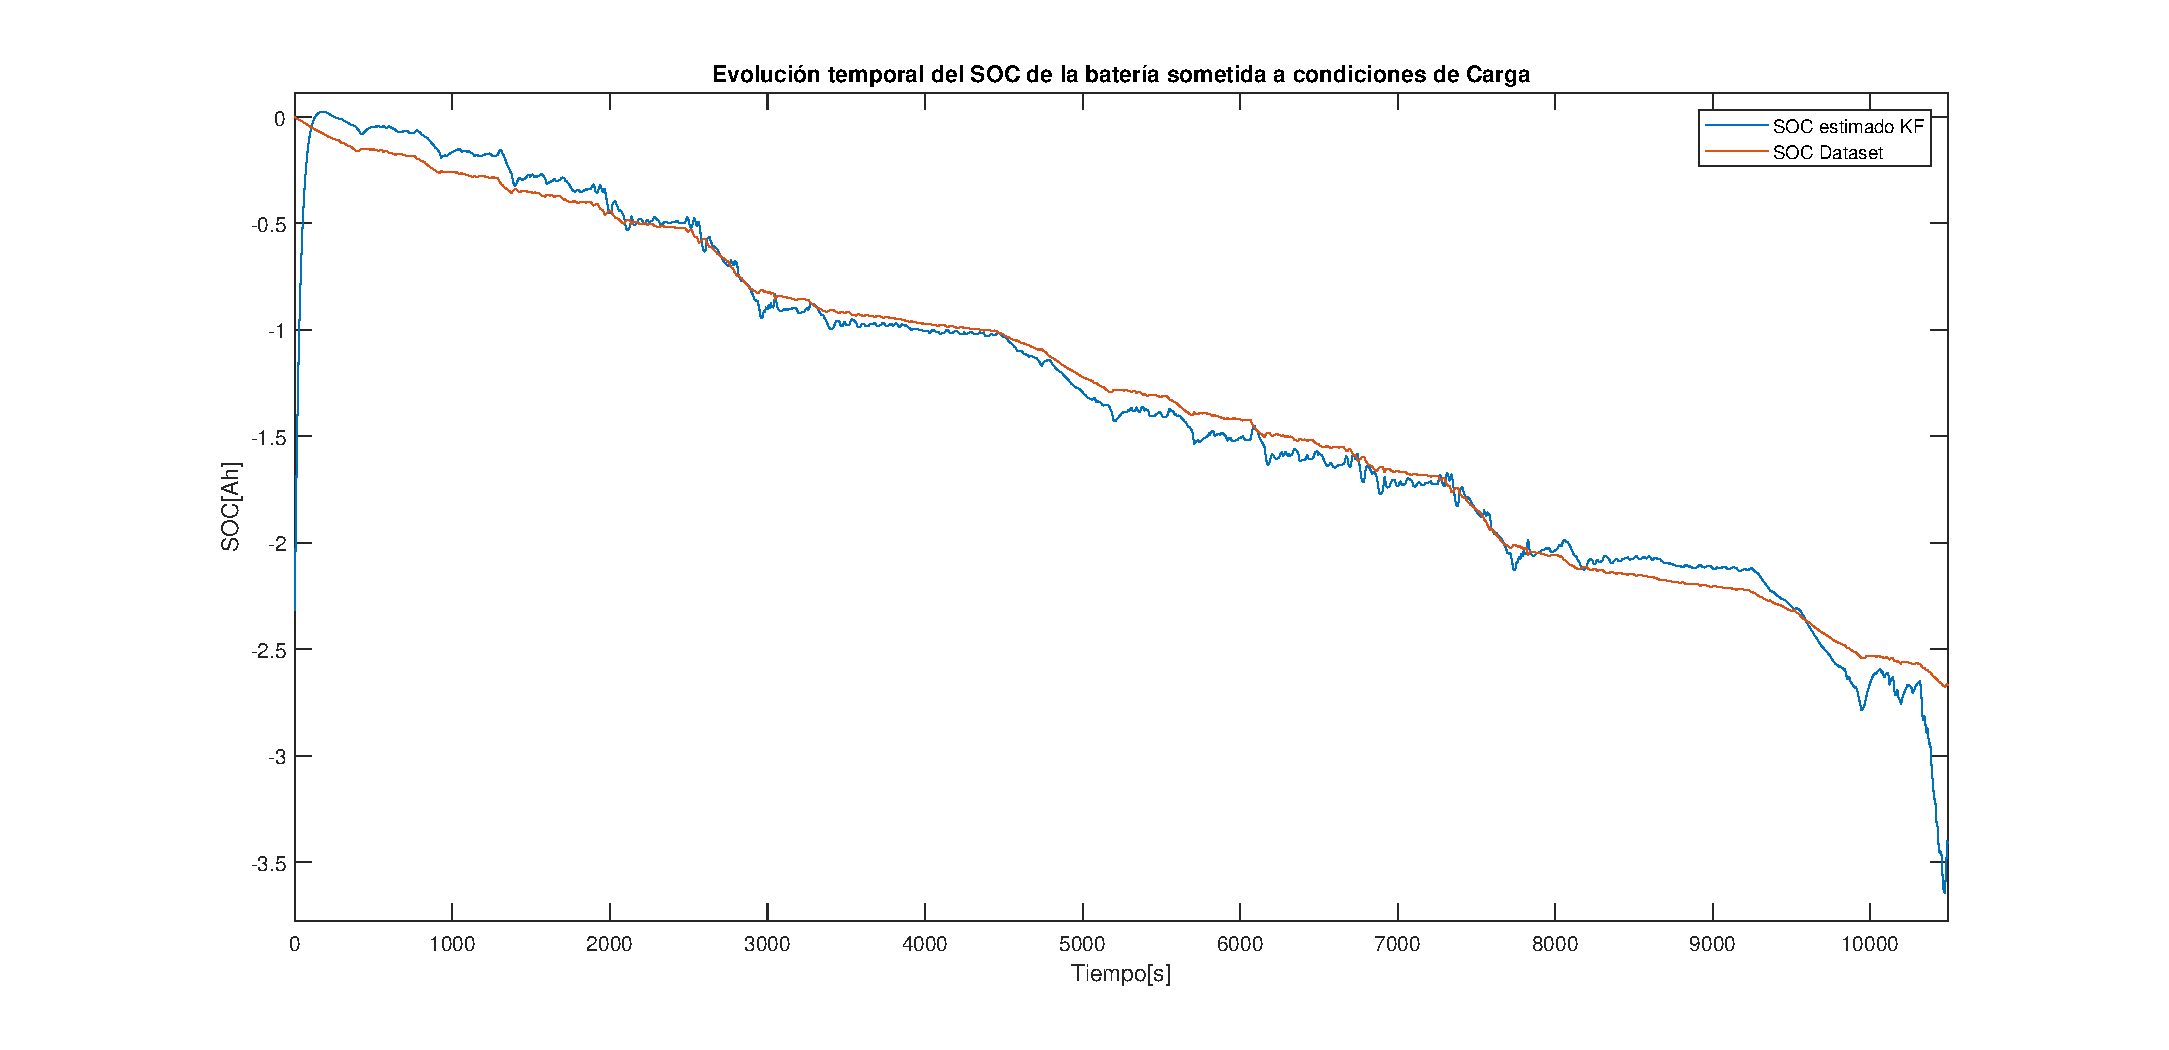
\includegraphics[width=0.95\textwidth]{Drive_Cycle_1_sim.eps}
	\caption{Resultados de la Simulación del sistema sometido a condiciones de
	ciclo de manejo}
	\label{Drive_Cycle_1_SOC_sim}
    \end{center}
\end{figure}

\begin{figure}[h!]
    \begin{center}
	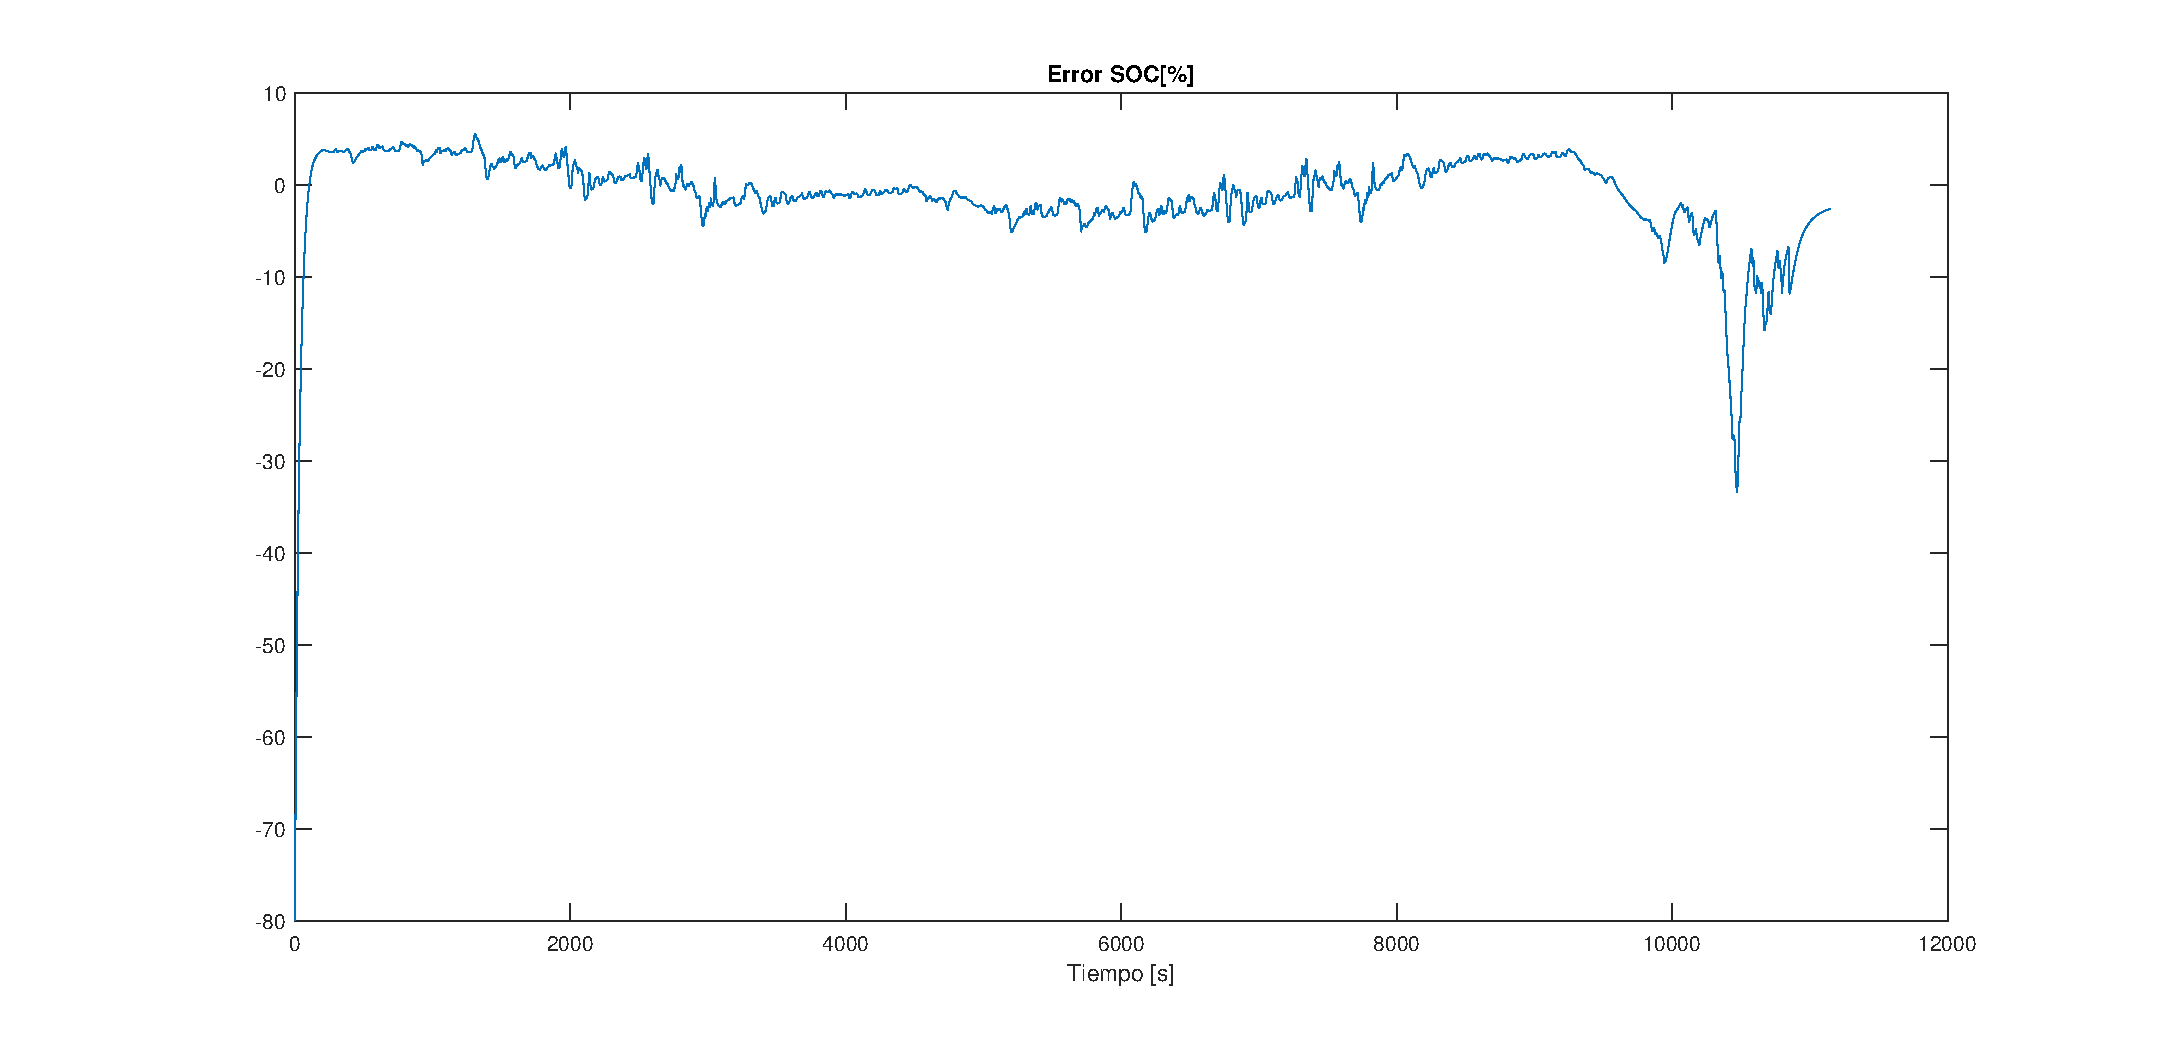
\includegraphics[width=0.95\textwidth]{soc_error_porc.eps}
	\caption{Resultados de Simulación del SOC de una batería sometida a
	condiciones de ciclo de manejo}
	\label{error_SOC_Sim}
    \end{center}
\end{figure}
\FloatBarrier

\subsection{Técnica de Carga} 
\subsubsection{Corriente Constante CC - Voltaje Constante CV}

El proceso de carga de una \acrfull{Ion-Li} no es trivial. Aplicar una tensión
constante en  bornes, como podríamos proceder con baterias de plomo ácido, no es
el procedimiento más adecuado en este caso. En aras de optimizar la autonomía y
la vida útil del pack de baterías el proceso de carga debe responder a
lineamientos particulares deacuerdo a las carácterísticas constructivas de las
celdas que lo componen.

El peril de carga que se ajusta a las celdas de \acrshort{Ion-Li}, como se
observa en la figura \ref{fig:char_prof}, es el perfil \acrfull{CC} -
\acrfull{CV}. Este consiste en tres fases, una primera etapa de
acondicionamiento o pre carga donde se inyecta a la batería una corriente
constante pequeña de magnitud equivalente a la corriente de fin de carga. Una
fase de carga rápida a corriente constante \acrshort{CC} y una tercer y última
fase de carga a tensión constante \acrshort{CV}.

\begin{figure}[h!] \centering
    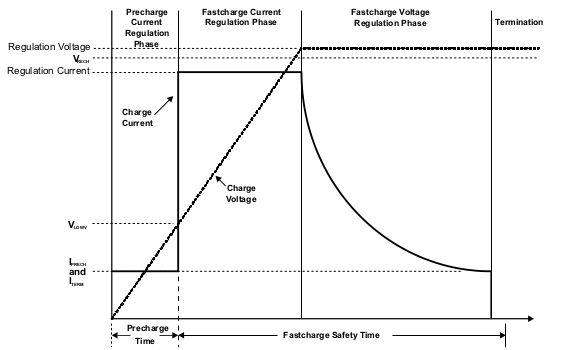
\includegraphics[width=0.8\textwidth]{bat_char/char_profile.png}
    \caption{Perfil de carga típico de una batería de Ion-Litio}
\label{fig:char_prof} \end{figure} \FloatBarrier

El proceso de pre carga o pre-acondicionamiento proporciona a las celdas la
capacidad de recuperar su capa de pasivación, la cual puede haberse visto
afectada o disuelta tras largos periodos de almacenamiento en estados de
descarga profunda. A su vez permite introducir las celdas en la zona de
operación segura en caso de que se encuente prufundamente descargadas.  Es
importante limitar el proceso de acondicionamiento en tiempo para prevenir pre
cargar indefinidamente una celda que se encuentre agotada. Si tras un periodo
completo de acondicionamiendo la celda no alcanza el voltaje mínimo necesario
puede considerarse que la misma alcanzó el final de su vida útil.

El voltaje umbral de inicio de carga rápida depende de la celda misma y en el
caso de las baterías \acrshort{Ion-Li} se ubica generalmente entre los $2.5V$ y
$3.0V$.  Una vez que la celda supera su voltaje umbral mínimo el cargador debeŕa
entra en la zona de carga rápida a corriente constante \acrshort{CC}. La fase de
carga rápida permite a la batería transformar la enería eléctria entregada en
energía electroquímica dentro de la batería en el menor tiempo posible. La
magnitud de la corriente de carga rápida depende de la celda y es limitada
generalmente entre $0.5C$ y $1C$ para prevenir el calentamiento del pack y su
degradación prematura. El pack de batería admitrá carga rápida a corriente
constante hasta alcanzar el voltaje límite de regulación. 

En esta tercer y última fase la corriente drenada del pack decae
exponencialmente hasta alcanzar la magnitud de fin de carga, situación que nos
indica que el ciclo se completo exitosamente. La corriente de terminación de
carga ronda entre $5\%$ y $10 \%$ de la corriente de carga rápida. Cabe aclarar
que en esta instancia del proceso de carga la corriente decae naturalmente dado
que es la contante de voltaje de terminales la magnitud controlada por el
cargador.  

Es importante remarcar que durante todo el proceso de carga, pero
fundamentalmente durante la fase de carga rápida a corriente constante, es de
vital importancia monitorear la temperatura de las celdas evitando que las
mismas se aparten de la zona de operación segura. Si bien el proceso de carga
implica intrínsicamente una elevación de la temperatura de la celda, etre otras
causas debido a su resistencia interna.

El tiempo total de carga es una variable determinante a la hora de implementar
un cargador de batería que extienda al máximo la vida útil y los ciclos de carga
de un pack de baterías y de sus celdas. Es la magnitud de corriente de carga
rápida la variable determinante del tiempo final de carga. Por ejemplo, para una
carga rápida a 1C, la bateria alcanzará, durante la fasé de \acrshort{CC}, el
$70\%$ de su capacidad total en el $30\%$ del tiempo de carga mientras que
tardará el $70\%$ del tiempo total de carga para acumular el $30\%$ restante de
su capacidad durante la fase \acrshort{CV}. 

La existencia de una resistencia interna en serie en las celdas no ideales
implica que a mayor corriente de carga rápida a CC se alcance más rápido la
tensión de umbral de paso a la fase de tensión constante CV acortando el tiempo
de CC pero extendiendo el tiempo de CV. Podemos inferir entonces que a menor
resistencia interna menor tiempo de carga. Y que aumentar la corriente a CC
tambien reducirá el tiempo de carga.  Sin embargo, se desaconseja completamente
implementar regímenes de carga rápida que superen 1C por el impacto en el número
de ciclos de vida útil de las celdas del pack de batería. La figura
\ref{fig:C_vs_Cycle_I} muestra como a medida que aumentamos el régimen de carga
\begin{figure}[h!] \centering
    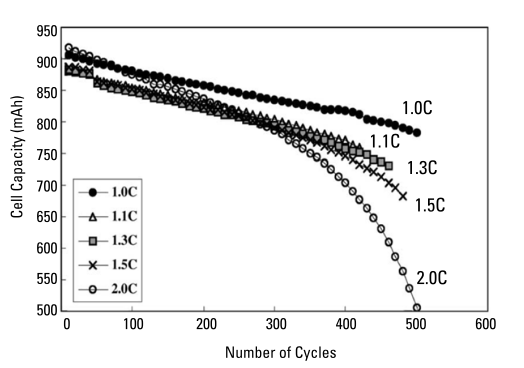
\includegraphics[width=0.6\textwidth]{bat_char/C_vs_Cycle_I.png}
    \caption{Relación Corriente de carga vs Ciclos de vidaútil de una celda de
    Ion-Litio con un cátodo de $LiCoO_2$} \label{fig:C_vs_Cycle_I} 
\end{figure}
\FloatBarrier

A mayores tasas de corriente, mayor cantidad de iones de litio se depositan
sobre el ánodo conviritiendose en litio metálico al librerar sus electrónes
disponibles.  El litio metálico es sumamente reactivo con el electrolito
resultando en una pérdida permanente de \acrshort{Ion-Li}, el elemento
almacendor de la energía, acelerando el evenjecimiento prematuro de la celda y
en consecuencia reduciendo los ciclos de vida útiles de la misma. 

Normalmente, a mayor voltaje en bornes de una celda mayor es la capacidad de la
misma. Podríamos entonces vernos tentados a aumentar el voltaje límite de
regulación y sobre cargar una celda para aumentar la carga almacenada. Por
ejemplo, una celta cargada a $4.3V$ en vez de $4.2V$ va a permitirnos almacenar
un $10\%$ más de carga inicial. El inconveniente aqui reside nuevamente en el
impacto que tendra estre procedimiento en el número de ciclos de carga y la vida
útil de la celda. La vida útil de una celda sobre cargada se vería reducida en
un $50\%$.  Por el otro lado, cargar una celda con un un voltaje menor ($40mv$
menor) implicará una reducción aproximada de un $10\%$ de su carga inicial.
Podemos arribar a la conclusión que el control del voltaje de carga y su
precisión es de vital importancia en un circuito de carga. La figura
\ref{fig:C_vs_Cycle_V} muentra la relación entre el número de ciclos de carga y
los diferentes voltajes de carga. 

\begin{figure}[h!] \centering
    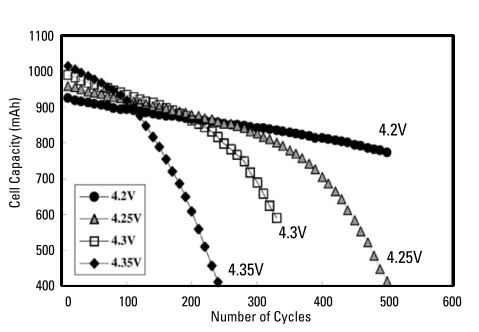
\includegraphics[width=0.6\textwidth]{bat_char/C_vs_Cycle_V.png}
    \caption{Relación Voltaje de carga la bateria vs Ciclos de vida de una celda de
Ion-Litio con un cátodo de $LiCoO_2$} \label{fig:C_vs_Cycle_V} \end{figure}
\FloatBarrier

A voltajes mayores el material del cátodo reacciona a mayor velocidad con el
electrolito perdiéndose material en la reacción resultando en una perdida de
capacidad de almacenamiento de energía. 

\subsubsection{Tecnología Seleccionada}

Para un completo control del perfil de carga ariba descripto es que
seleccionamos circuito integrado \emph{bq24610} de la firma \emph{Texas
Instrument}.

El \emph{bq24610} es un circuito altamente integrado que implementa un cargador
de \acrfull{Ion-Li} o \acrfull{Li-Po} y capaz de operar de forma independiente o
stand-alone. Emplea un controllador de corriente y de tensión sincrónico
switching PWM de frecuencia constante y de alta resolución del tipo buck cuya
topología simplificada puede observarse en la figura \ref{fig:simp_sch_char}. 

\begin{figure}[h!]
    \centering
    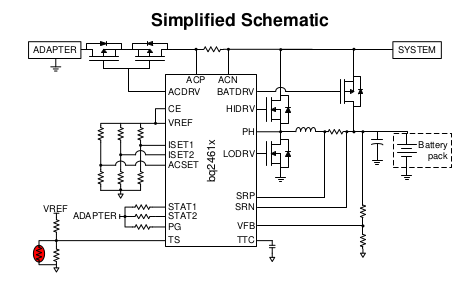
\includegraphics[width=0.5\textwidth]{bat_char/simp_sch_char.png}
    \caption{Esquema simplificado Cargador de Batería}
    \label{fig:simp_sch_char}
\end{figure}
\FloatBarrier

El mismo admite la conexión de hasta 6 celdas en serie con una tensión y
corriente máxima de entrada de hasta $28V$ y $10A$ respectivamente y una salída
de hasta $26V$ y $10A$ ajustandose adecuadamente a nuestros requerimientos y a
la topología de nuestro pack de baterías \emph{6S3P} descripta en \ref{batSel}.
El empaquedato del mismo es del tipo VQFN.

\subsection{Ecualización de celdas}

\noindent Como se comentó en secciones anteriores, cuando múltiples celdas se
encuentran conectadas en serie, el voltaje de una celda no siempre coincide con
la tensión equivalente del pack de baterías dividido por el número de celdas. 

\noindent La ecualización de celdas es una técnica en la cual se trata de
mantener los niveles de voltaje entre las celdas que conforman la cadena
conectada en serie de un pack de baterías de forma homogénea, es decir, que los
niveles de tensión entre celdas sea lo más uniforme posible, con el objetivo de
maximizar la eficiencia del pack de baterías.

\noindent El desbalance más típico generalmente se manifiesta en una variación
en el voltaje entre éstas, que puede ser corregido instantáneamente o
gradualmente conectando cargas externas en paralelo, a través de sus
correspondientes transistores, provocando una corriente de descarga adicional
que pueden ir desde miliamperes hasta varios Amperes, dependiendo del
dimensionamiento energético del pack de baterías. Sin embargo, este desbalance
en tensión es, por lo general, dado por desbalances químicos o distintas
dinámicas de descarga entre celdas, provocando que el objetivo del balanceo no
esté claramente definido provocando más perjuicios que beneficios al sistema
completo.  De hecho, la mayoría de las metodologías basadas en el desbalance de
voltaje, llevan a un pack de baterías más desbalanceado que sin ellos.

\noindent Por lo tanto es necesario conocer la naturaleza de los distintos tipos
de desbalances, los cuales son descriptos a continuación:

\subsubsection{Desbalance del estado de carga (SoC)}

\noindent El desbalanceo por estado de carga es causado por celdas que son
cargadas a distintos nivels de \acrshort{SOC}. Por ejemplo, si tenemos 3 celdas
cuya carga máxima es de 2200mAh ($\mathrm{Q_{max}}$), y descargar 100mAh una de
las celdas ($\mathrm{Q_1}$), la segunda por 100mAh y la tercera por 200mAh , la
primer y segunda celda van a estar a un \acrshort{SOC} de
$\mathrm{\frac{(Q_{max} - Q_1)}{Q_{max}} = 95.4\%}$. pero la tercer celda
estará, a cálculo hecho, en un 91\%. Por lo que podemos decir que la tercer
celda presenta un desbalance de un 4.4\%. 

Esto se traduce en distintos voltajes de circuito abierto, ya que se encuentran
directamente correlacionadas con el estado de carga de las mismas, sin embargo,
a pesar de esta diferencia constante de \acrshort{SOC}, la tensión entre celdas
varía con el crshort{SOC} debido a su variación con respecto a los distintos
niveles de estado de carga. En la Figura \ref{diff_imbalance} se muestra como
varía la diferencia de voltaje entre las celdas ante distintos niveles de
crshort{SOC} con un desbalance constante teniendo en cuenta la curva de la
figura \ref{OCV_SOC_equalization_figure}.

\begin{figure}[h!]
    \begin{subfigure}[t]{.5\textwidth}
	\begin{center}
	    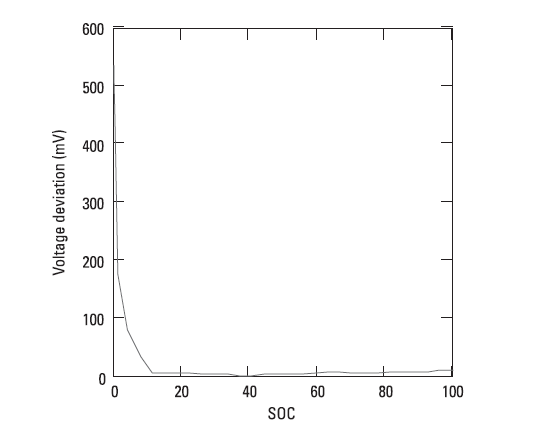
\includegraphics[width=0.9\textwidth]{diff_imbalance.png}
	    \caption{Diferencia de OCV a distintos estados de carga para un desbalance
	    de 1\% de SOC}
	    \label{diff_imbalance}
	\end{center}
    \end{subfigure}%
    ~
    \begin{subfigure}[t]{.5\textwidth}
	\begin{center}
	    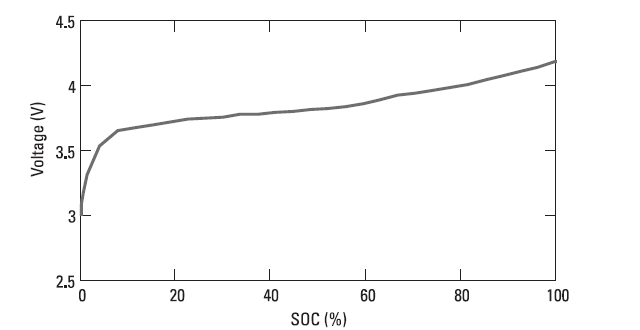
\includegraphics[width=0.9\textwidth]{SOC_vs_OCV_equalization.png}
	    \caption{OCV vs SOC}
	    \label{OCV_SOC_equalization_figure}
	\end{center}
    \end{subfigure}
    \caption{Variaciones del OCV segun SoC}
    \label{rep_OCV_SOC}
\end{figure}
\FloatBarrier

\noindent El voltaje sobre una carga puede ser aproximadamente, y rápidamente,
modelada por la siguiente ecuación:



\noindent Debido a que la función $R(SOC)$ incrementa rápidamente a bajos
valores de SOC, la diferencia de voltajes entre celdas, con un desbalance de SOC
determinado, incrementa en un estado de carga muy bajo sugeriendo que existe un
incremento en la necesidad de realizar el proceso de balanceo cuando el pack de
baterías alcanza su descarga completa, sin embargo, si esta diferencia de SOC es
eliminada en etapas anteriores, las diferencias de tensión que ocurren cerca del
fin de descarga son eliminadas sin necesidad de altas corrientes de drenaje para
cada celda.

\subsubsection{Diferencias entre impedancias internas}

La diferencia entre impedancias internas en un bache de producción es de
aproximadamente un 15\% como se puede observar en la Figura \ref{zin_diff}.

\begin{figure}[h!]
    \begin{center}
	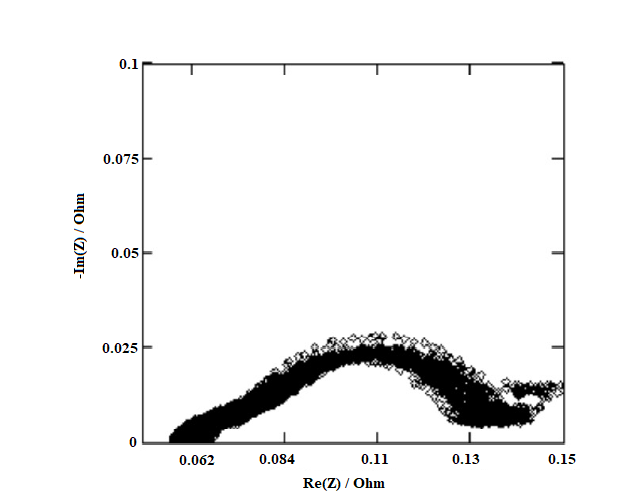
\includegraphics[width=0.7\textwidth]{zin_diff.png}
	\caption{Diferencias de espectrometrías entre 50 celdas. 
	El ensayo es realizado entre 1kHz a 10mHz}
	\label{zin_diff}
    \end{center}
\end{figure}
\FloatBarrier

Desbalances en la impedancia interna de la celda no causan diferencias en el
OCV, sin embargo, causará diferencias en el voltaje de la celda durante la
descarga, ya que la misma viene dada por la Ecuación \ref{v_load_bat}. Si la
batería se encuentra descargando, es decir, si la corriente es negativa el
voltaje que entrega a la carga será menor para una celda con mayor impedancia
interna. Por el otro lado, si la celda se encuentra cargando, el voltaje será
mayor para aquellas celdas con mayor resistencia interna.

A pesar de estas diferencias, no hay mecanismo de balanceo que permita solventar
el problema del desbalanceo de impedancia interna.

\subsubsection{Diferencias en la Capacidad de las celdas}

Por el otro lado, puede suceder que la capacidad química de las celdas
($\mathrm{Q_{MAX}}$) pueden ser diferentes en un principio, esto provoca que, a
pesar de que cada celda sea descargada por la misma cantidad de corriente, el
estado de carga será diferente. Por ejemplo, si las 3 celdas que nombramos
anteriores son descargadas por 100mAh, pero la 3er celda tiene una capacidad
distinta al resto (por ejemplo, 2000mAh en vez de 2200mAh), los estados de carga
resultantes serán de 95.4\% y 95\%.

Nuevamente esto provocará una diferencia en los OCVs de las celdas. Como puede
observarse, 200mAh de diferencia en $\mathrm{Q_{MAX}}$ causa solamente una
diferencia de un 0.4\% en el SOC, causando menor diferencia de voltaje que un
desbalance en el estado de carga.

Teniendo esto en cuenta las baterías no podrán estar balanceadas durante todo el
ciclo de descarga o de carga ya que al quitar la misma cantidad de carga el
estado de carga de las mismas será distinto. Un ejemplo algo más gráfico de esto
es con 2 vasos de agua, uno con el doble de capacidad del otro pero llenos hasta
la misma altura. Si se remueve la misma cantidad de agua de ambos el de mayor
capacidad se habrá descargado la mitad que el de menor capacidad.

En la práctica lo más común es lo que se llama \emph{top balancing}, que implica
balancear en el período de carga todas las celdas del pack al 100\%. El mismo
consiste descargar las celdas de menor capacidad permitiendo a las celdas de
mayor capacidad un margen para seguir cargando sin sobrecargar las primeras,
evitando lo que generaría una drástica disminución de la vida útil del pack.
Esta opción es mucho más atractiva que su contra parte denominada \emph{bottom
balancing} ya que esta balancea todas las baterías a su estado de carga en 0\%,
lo cual no acarrea ninguna ventaja ya que el pack de baterías va a seguir
entregando a la carga la misma cantidad de energía, esto es, cuando la batería
de menor capacidad se descargue como pasaría si no se realizara el balanceo
inferior.

La descarga de las celdas se puede llevar a cabo disipando su energía en
resistores o transfiriendo la carga a las celdas más descargadas, siendo estos
métodos clasificados como balanceo pasivo o balanceo activo respectivamente. Los
métodos pasivos son mucho más sencillos y económicos y en la mayoría de los
casos no es justificado el uso del método activo ya que los circuitos que llevan
a cabo la transferencia de energía poseen perdidas por lo que no ofrecen
ventajas reales en aplicaciones de baja potencia.

Por el otro lado, puede suceder que la capacidad química de las celdas
($\mathrm{Q_{MAX}}$) pueden ser diferentes en un principio, esto provoca que, a
pesar de que cada celda sea descargada por la misma cantidad de corriente, el
estado de carga será diferente. Por ejemplo, si las 3 celdas que nombramos
anteriores son descargadas por 100mAh, pero la 3er celda tiene una capacidad
distinta al resto (por ejemplo, 2000mAh en vez de 2200mAh), los estados de carga
resultantes serán de 95.4\% y 95\%.

Nuevamente esto provocará una diferencia en los OCVs de las celdas.  Como puede
observarse, 200mAh de diferencia en $\mathrm{Q_{MAX}}$ causa solamente una
diferencia de un 0.4\% en el SoC, causando menor diferencia de voltaje que un
desbalance en el estado de carga.

Teniendo esto en cuenta las baterías no podrán estar balanceadas durante todo el
ciclo de descarga o de carga ya que al quitar la misma cantidad de carga el SoC
de las mismas será distinto. Un ejemplo algo más gráfico de esto es con 2 vasos
de agua, uno con el doble de capacidad del otro pero llenos hasta la misma
altura. Si se remueve la misma cantidad de agua de ambos el de mayor capacidad
se habrá descargado la mitad que el de menor capacidad.

En la práctica lo más común es lo que se llama \emph{top balancing}, que implica
balancear en el período de carga en la que el pack se considera cargado a un
100\% o durante el periodo de Tension constante o CV (del ingles \emph{Constant
Voltage}). El mismo consiste descargar las celdas de menor capacidad permitiendo
a las celdas de mayor capacidad un margen para seguir cargando sin sobrecargar
las primeras, evitando lo que generaría una drástica disminución de la vida útil
del pack. Esta opción es mucho más atractiva que su contra parte denominada
\emph{bottom balancing} ya que esta balancea todas las baterías a su estado de
carga cercano al 0\%, lo cual no acarrea ninguna ventaja ya que el pack de
baterías va a seguir entregando a la carga la misma cantidad de energía, esto
es, cuando la batería de menor capacidad se descargue como pasaría si no se
realizara el balanceo inferior.

La descarga de las celdas se puede llevar a cabo disipando su energía en
resistores o transfiriendo la carga a las celdas más descargadas, siendo estos
métodos clasificados como balanceo pasivo o balanceo activo respectivamente. Los
métodos pasivos son mucho más sencillos y económicos y en la mayoría de los
casos no es justificado el uso del método activo ya que los circuitos que llevan
a cabo la transferencia de energía poseen perdidas por lo que no ofrecen
ventajas reales en aplicaciones de baja potencia.

Por último hay que considerar que corriente es necesaria para balancear el pack,
a mayor capacidad de corriente las corrientes de auto descarga y cambios en la
capacidad por envejecimiento van generando pequeños desbalances, pero los mismos
son acotados, las corrientes de auto descarga generan desbalances menores al
0.1\% por ciclo. 

\begin{figure}[h!]
    \begin{center}
	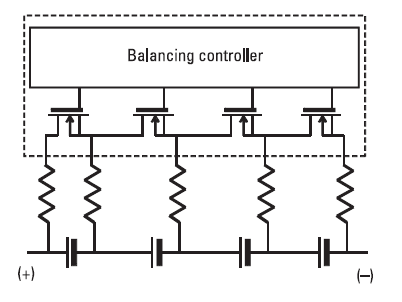
\includegraphics[width=0.5\textwidth]{passive_equalizator.png}
	\caption{Esquemático de conexión de un balanceador pasivo.}
	\label{passive_equalizator}
    \end{center}
\end{figure}
\FloatBarrier

%Para la implementación del balanceador analizó LTC6803-2.

El integrado BQ76PL536 de texas instrument es un Monitor de batería con
protecciones para sobre  y sub tensión y sobrecalentamiento asi como también
posee varias funcionalidades entre las cuales se destacan la posibilidad de
escalar el número de celdas en serie gracias a su interfaz D2D VBUS
(\emph{device to device vertical BUS}) permitiendo la conexión en serie de
varios BQ76PL536 permitiendo controlar hasta 6 celdas por integrado hasta un
total de 192 celdas.
%Anteriormente se nombró la importancia de la protección de las celdas, ya que
%el voltaje de ruptura del electrolito es cercano a la tensión de carga máxima
%de una celda (entre 4.1V a 4.3V por celda). Por lo tanto, se debe realizar un
%control y monitoreo riguroso para que las celdas de un pack experimente un
%sobrevoltaje durante el proceso de carga. Esto, conlleva a que, en un pack de
%baterías, cada celda sea monitoreada y controlada por separado, ya que
%controlar la tensión del pack de baterías no es suficiente, debido a que, a
%pesar de que los valores pueden encontrarse dentro de un umbral correcto, una
%de las celdas que componen el sistema puede estar experimentando un daño
%permanente por sobrevoltaje debido al desbalance que pueden encontrarse entre
%celdas

%El balanceo de celdas es necesario para aquellas aplicaciones donde tienen
%grandes transitorios de energía, especialmente aquellas aplicaciones donde
%ocurre frecuentemente, como por ejemplo, los frenos regenerativos en los EVs y
%HEVs. El freno regenerativo puede causar grandes flujos de corriente provocando
%un incremento instantáneo en la tensión de cada celda, alcanzando la tensión de
%ruptura del electrolito.

%Las desviaciones en las celdas generalmente ocurren debido a dos fenómenos:
%cambios en la impedancia interna o en la reducción de capacidad debido al
%envejecimiento de las mismas. En ambos casos, si una celda experimenta una
%desviación en su comportamiento, esta celda es un posible candidato a un
%sobrevoltaje durante los eventos que ocurren los transitorios de potencia. Las
%celdas con capacidad reducida o alta impedancia interna tienden a tener altas
%variaciones de tensión durante los procesos de carga y descarga.
%
%Por último, en aplicaciones donde es deseable obtener la mayor capacidad usable
%de un pack de baterías, puede ocurrir que durante el proceso de carga, una
%celda desbalanceada alcance el voltaje de fin de carga y provoca que el proceso
%de carga termine prematuramente. Entonces, además de proteger el pack de
%baterías, el proceso de carga permite aprovechar la capacidad completa del pack
%a pesar de los desbalanceos intrínsecos de cada celda.
%
%Tradicionalmente, los desbalances entre celdas en baterías de plomo son
%solucionados por una sobrecarga controlada. Este tipo de baterías pueden ser
%llevadas a condiciones de sobrecarga sin ser dañadas permanentemente, ya que el
%exceso de energía es liberado a través de la gasificación de las sustancias
%químicas que contienen. Éste método, es el método natural para el balanceo de
%celdas de plomo-ácido conectadas e nserie. Otras composiciones químicas, tales
%como las de Niquel-metal, exhiben un mecanismo similar.
%
%Debido a que las baterías de Litio no pueden ser sobrecargadas, no existe un
%mecanismo natural para el balanceo de celdas. Por lo tanto, se deben emplear
%métodos diferentes para balancearlas. Los métodos de balanceo se pueden separar
%en dos grandes grupos: Métodos activos y pasivos.
%
%A continuación, se describen los métodos más comunes para realizar el balanceo
%de celdas.

%\subsubsection{Balanceo de Celdas en el Fin de carga}

%Este método es empleado cuando el pack de baterías cuando es cargada
%completamente y es, generalmente, implementada en aquellas aplicaciones en las
%cuales el pack de baterías es completamente cargado en cada ciclo de su uso.
%Como pueden ser en fuentes de baterías ininterrumpidas (UPS, del inglés
%\emph{Uninterruptible Power Supply}) o vehículos eléctricos hasta celulares. 





\subsection{Plan de Trabajo}

Se plantea el siguiente plan de trabajo con el tiempo estimado para la
finalización del proyecto:

\begin{table}[h!]
    \begin{tabular}{|l|c|}
	\hline
	\multicolumn{1}{|c|}{Tarea}                                                                                                                                                                              & Duración                           \\ \hline
	\begin{tabular}[c]{@{}l@{}}Estudio, análisis y comparación del estado del arte de la tecnología. \\Estudio de los requerimientos de hardware.\end{tabular}                         & 2 Semanas                          \\ \hline
	    \begin{tabular}[c]{@{}l@{}}Modelado de baterías de Li-Ion en MatLab. \\Simulación de los distintos algoritmos y los circuitos de protección. \\ Estudio y comparación. Validación y elección de los más adecuados.\end{tabular} & 4 Semanas                          \\ \hline
		\begin{tabular}[c]{@{}l@{}}Desarrollo e implementación del hardware del \acrshort{BMS}. *\end{tabular}                                                      & 6 Semanas                          \\ \hline
		    \begin{tabular}[c]{@{}l@{}}Desarrollo del Firmware del \acrshort{BMS} con los algoritmos seleccionados.\\  Implementación y depuración sobre el hardware.\end{tabular}                                                    & 4 semanas                          \\ \hline
			Montaje del banco de pruebas para ensayar las protecciones y los algoritmos correspondientes. *                                                                                                                       & 3 Semanas                          \\ \hline
			Análisis de resultados, obtención de conclusiones y desarrollo del informe final.                                                                                                                                                       & 3 Semanas                          \\ \hline
			\textbf{Total}                                                                                                                                                                                                  &\textbf{24 Semanas} \\ \hline
    \end{tabular}
\end{table}

\subsection{Extensión a futuros proyectos}

El desarrollo del hardware y los algoritmos, tanto de ecualización como de
estado de carga sirven como una buena base para futuros proyectos vinculados a
la temática de energías renovables y \acrshort{VE}s.

Como posible extensión se plantea el desarrollo de algoritmos novedosos para la
estimación del Estado de Salud, su posible aplicación a sistemas de alta
potencia e inclusive realizar estudios sobre nuevas tecnologías relacionadas a
la composición química de las celdas.

\newpage

\section{Desarrollo}\label{desarrollo}


(insertar somewhere):
\subsection{Tiempo de Muestreo}
Al trabajar con estrategias de control basadas en microcontroladores y sensores digitales nos encontramos con la necesidad de discretizar los procesos y tener en cuenta los tiempos de muestreo.

El teorema de Nyquist-Shannon nos permite calcular un límite inferior a la frecuencia de muestreo, ya que este establece que si la frecuencia de muestreo cumple con la condición \ref{nyquist_condition} siendo $f_s$ la frecuencia de muestreo y $F_{MAX}$ la máxima frecuencia presente en la señal, se podrá reconstruir la señal sin perder información.
Por el contrario, si la señal y la frecuencia de muestreo no son las adecuadas se produciría \emph{aliasing}.\\
\begin{equation}
	f_s > 2 F_{MAX}
	\label{nyquist_condition}
\end{equation}


Dado el sistema de ecuaciones \ref{SS_model_eq} el cual es una representación de nuestro sistema en espacio de estados, podemos calcular los valores de los polos sabiendo los Eigenvalores o Autovalores de la matriz de evolución A.\\
Además, la matriz de evolución de nuestro sistema es diagonal por lo que los autovalores y subsecuentemente los polos se corresponden con los elementos $A_{nn}$ con $n=\{1;2;3\}$.\\ 

Tomando el valor del máximo valor absoluto entre los elementos $A_{nn}$ de las todas matrices A obtenidas para cada valor de $SoC$ obtuvimos de la ecuación \ref{eq_polo_rapido}, el valor del polo más rapido:

     \begin{equation}
     	MAX  \left \|A_{nn}(Soc)\right \| = \omega = 6.6379 rad/s
     	\label{eq_polo_rapido}
     \end{equation}


Dado que la frecuencia de corte $f_c$ asociada al polo más rapido se calcula según la ecuación \ref{ang_vs_frec} obtenemos $F$ y reemplazamos en \ref{nyquist_condition} obteniendo nuestra frecuencia mínima de muestreo $f_{smin}$ de la ecuación \ref{nyquist_condition2}.

\begin{equation}
	F = \frac{\omega}{2 \pi} = 1.056 Hz
	\label{ang_vs_frec}
\end{equation}

\begin{equation}
	f_{s min} > 2 F = 2.113 Hz
	\label{nyquist_condition_2}
\end{equation}

En la figura \ref{system_bode} se observa que a partir de $\omega = 10 rad/s$ la ganancia esta determinada por $-20log(R_{0})\approx-30dB$, lo cual es coherente con los calculos previos.\\

\begin{figure}[h!]
	\begin{center}
		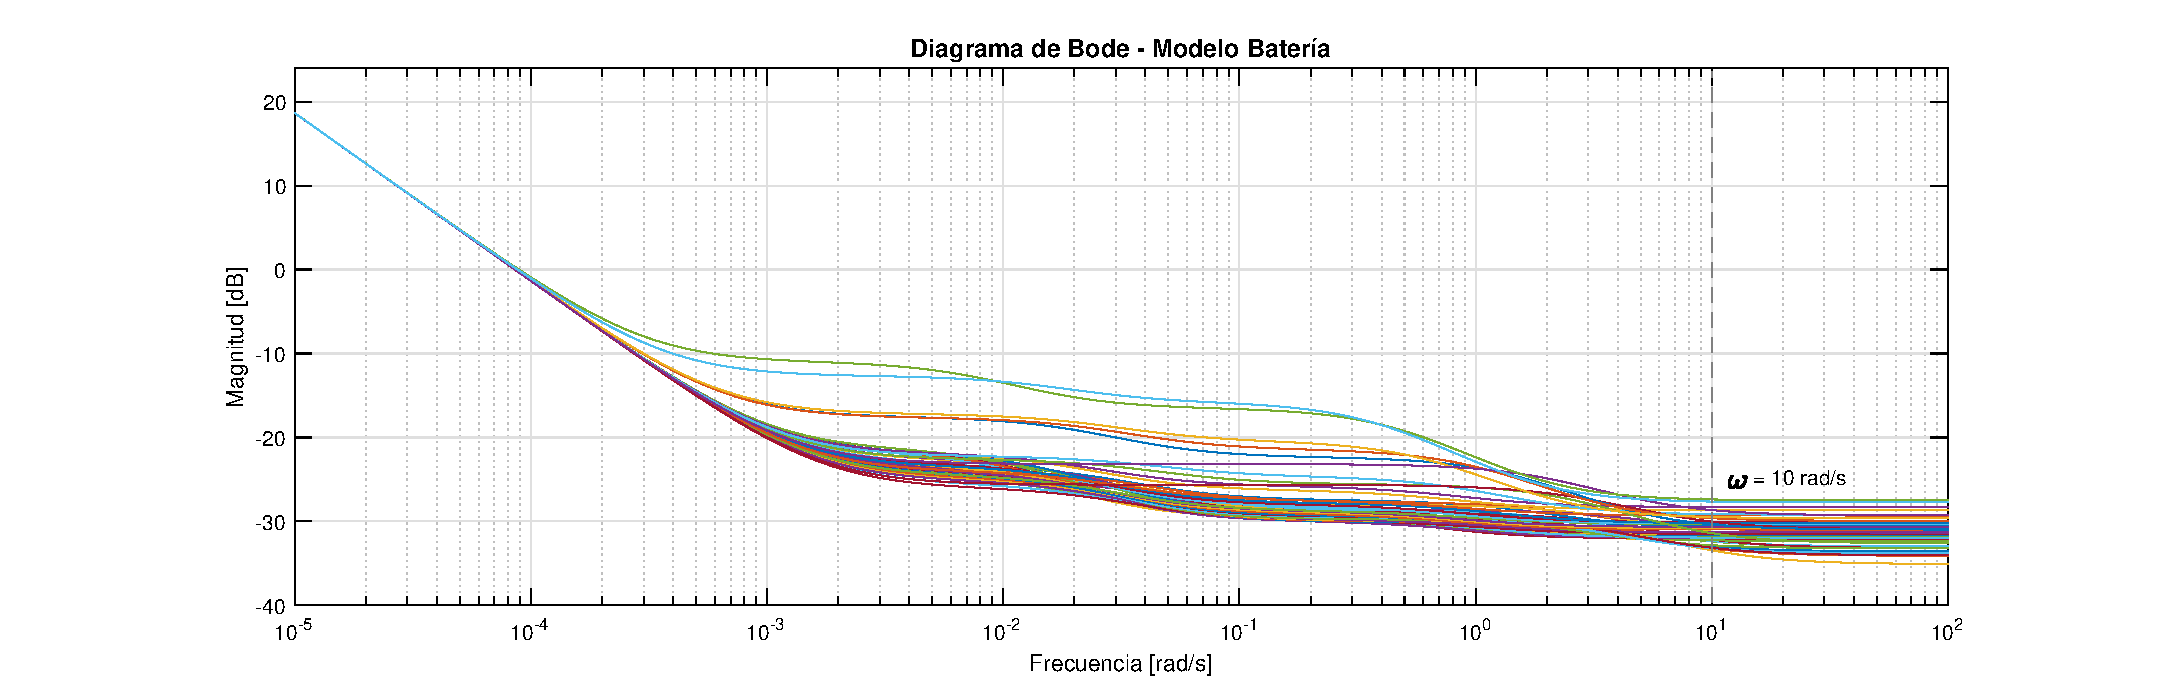
\includegraphics[width=1\textwidth]{bode_amplitud_w_grid.eps}
		\caption{Diagrama de Bode del sistema.}
		\label{system_bode}
	\end{center}
\end{figure}

Los tiempos de procesamiento del Microcontrolador del filtro de Kalman y los sensores en conjunto son de 10ms por lo que la frecuencia de muestreo de nuestro sistema es $100 Hz$ cumpliendo con la condición \ref{nyquist_condition}.\\


\clearpage



%\subsection{Implementación Circuito Cargador}

% La carga del pack de batería no es un proceso trivial y la extensión de la
% vida util del mismo depende profundamente de poder controlar el mismo con
% detalle. 

% El control completo de la operación del pack de batPoder controlar Extender la
% vida util del pack de baterías no es un tema trivial como ya hemos expuesto
% anteriormente. El balanceo de carga es

\clearpage

\section{Ensayos}\label{ensayos}
(Sección en desarrollo)
%TODO: Ensayos
\newpage

\section{Conclusiones}\label{conclusiones}
(Sección en desarrollo)
%TODO: Conclusiones
\newpage

\appendix

\section{Desarrollo matem\'atico del Filtro de Kalman}\label{matKalman}

\noindent El filtro de Kalman es construido como un minimizador del error 
cuadr\'atico medio (o \acrshort{MSE}, del ingl\'es 
\emph{\acrlong{MSE}}), pero tambi\'en existe una derivaci\'on 
alternativa del filtro motrando como el mismo maximiza las estad\'isticas de 
probabilidad.

\noindent El prop\'osito de filtrar es extraer la informaci\'on requerida de una
señal, ignorando el resto. Evaluar el funcionamiento del filtro puede ser
realizado utilizando funciones de costo o p\'erdida, por lo tanto, podemos
definir que el objetivo del filtro es minimizar la funci\'on de p\'erdida (o en
ingl\'es, \emph{loss}).

\subsection{Error Cuadr\'atico Medio}

\noindent Las señales lineales pueden ser descriptas de la siguiente forma
(\emph{ec.\ref{lineal_signal}}):

\begin{equation}
    y_k = a_k x_k + n_k \label{lineal_signal}
\end{equation}

\noindent Donde $\mathrm{y_k}$ es la señal observada, $\mathrm{a_k}$ es la 
ganancia, $\mathrm{x_k}$ es la informaci\'on que lleva la señal y $\mathrm{n_k}$ 
es el ruido aditivo.

\noindent El objetivo del filtro es estimar $\mathrm{x_k}$. La diferencia entre
la estimaci\'on de $\mathrm{\hat{x}_k}$ y $\mathrm{x_k}$ se puede definir en la
Ecuaci\'on \ref{error_estimacion} como el error:

\begin{equation}
    f(e_k) = f(x_k - \hat{x}_k) \label{error_estimacion}
\end{equation}

La forma de $\mathrm{f(e_k)}$ depende de la aplicaci\'on, sin embargo, es claro
que la misma debe ser positiva y aumentar de forma monot\'onica. Una funci\'on
de error que exhibe estas caracter\'isticas es la funci\'on de error
cuadr\'atico (\emph{ec. \ref{error_cuadratico}}).

\begin{equation}
    f(e_k) = (x_k - \hat{x}_k)^2 \label{error_cuadratico}
\end{equation}

Dado que es necesario considerar la habilidad del filtro en predecir una
cantidad de informaci\'on determinada sobre un per\'iodo de tiempo, cobra mayor
sentido evaluar la m\'etrica de la funci\'on de error sobre el tiempo,
obteniendo la Ecuaci\'on \ref{loss_function}.

\begin{equation}
    lossfuncion = E\left(f(e_k)\right) \label{loss_function}
\end{equation}

Que esto resulta en la funci\'on \acrshort{MSE} (\emph{ec. \ref{mse}}).

\begin{equation}
    \epsilon(t) = E(e^2_k) \label{mse}
\end{equation}

\subsection{M\'axima Probabilidad}\label{maximum_likelihood_section}

La derivaci\'on del error cuadr\'atico medio, a pesar de ser intuitivo, se lo
considera de car\'acter heur\'istico. Una derivaci\'on m\'as rigurosa puede ser
desarollada usando la m\'axima probabilidad estad\'istica (o \acrshort{MLE}, del
ingl\'es \acrlong{MLE}). Esto es logrado redefiniendo el objetivo del filtro en
encontrar $\mathrm{\hat{x}}$ que maximiza la probabilidad de y. Que se define
matem\'aticamente en la Ecuaci\'on \ref{mle}.

\begin{equation}
    max\left[P\left(y|\hat{x}\right)\right] \label{mle}
\end{equation}

Asumiendo que el ruido aditivo es Gaussiano con una desviaci\'on estandard
$\mathrm{\sigma_k}$, obtenemos la Ecuaci\'on \label{probabilidad_y_x};

\begin{equation}
    P\left(y_k|\hat{x}_k\right) = K_ke^{\left(- \frac{(y_k - a_k\hat{x}_k)^2}{2\sigma^2_k}\right)} \label{probabilidad_y_x}
\end{equation}

Donde $\mathrm{K_k}$ es una constante de normalizaci\'on. La funci\'on de
m\'axima probabilidad Ecuaci\'on \ref{probabilidad_y_x} se encuentra expresada
en la Ecuaci\'on \ref{max_likelihood};

\begin{equation}
    P(y|\hat{x}) = \prod_k K_ke^{\left(- \frac{(y_k - a_k\hat{x}_k)^2}{2\sigma^2_k}\right)} \label{max_likelihood}
\end{equation}

Que lleva a la Ecuaci\'on \ref{derivation_mse};

\begin{equation}
    log[P\left(y|\hat{x}\right)] = - \frac{1}{2}\sum_k \left(\frac{(y_k -
    a_k\hat{x}_k)^2}{2\sigma^2_k}\right) + constante \label{derivation_mse}
\end{equation}

La funci\'on a la que deriva la Ecuaci\'on \ref{derivation_mse} es la
\acrshort{MSE}, que puede ser maximizada ante una variaci\'on de
$\mathrm{\hat{x}_k}$. Por lo tanto, el error cuadr\'atico medio es una funci\'on
aplicable cuando $\mathrm{y_k}$ es modelada con una distribuci\'on Gaussiana.
En tal caso el \acrshort{MSE} sirve para proveer el valor de
$\mathrm{\hat{x}_k}$ que maximiza la probabilidad de la señal $\mathrm{y_k}$.

En la pr\'oxima derivaci\'on se define el filtro \emph{\'optimo} como aqu\'el
filtro, de todos los posibles filtros que minimizan el \acrshort{MSE}.

\subsection{Derivaci\'on del Filtro de Kalman}

\noindent Al momento de desarrolar el filtro de Wiener, Wiener describe un 
filtro \'optimo de tipo respuesta al impulso finito, o \acrshort{FIR} (del 
ing\'es, \acrlong{FIR}) en el sentido del \acrshort{MSE}, utilizando la auto
correlaci\'on y la correlaci\'on cruzada de la señal recibida con la
informaci\'on original, para poder derivar la respuesta al impulso para el
filtro. 

\noindent Por el otro lado, Kalman presenta su filtro que logra optimizar el
\acrshort{MSE} pero a diferencia de que no necesita obtener la respuesta al
impulso para poder determinar el filtro. Kalman describe su filtro usando
t\'ecnicas basadas en el espacio de estados, lo que permite al filtro ser
utilizado como un \emph{suavizador} (o del ingl\'es, \emph{smoother}), un filtro
o un predictor. El uso del mismo como predictor, permiti\'o que el mismo sea
aplicado en un gran rango de aplicaciones para problemas de trackeo y
navegaci\'on. Definiendo el filtro en t\'erminos de un espacio de estados
tambi\'en simplifica la implementaci\'on del filtro en el dominio discreto, otra
raz\'on por la cual es utilizado ampliamente.

\subsubsection{Derivaci\'on a partir del espacio de estados}

\noindent Asumiendo que se quiere conocer el valor de una variable dentro de un 
proceso de la forma dada por la Ecuaci\'on \ref{system_eq}.

\begin{equation}
    x_{x+1} = Ax_k + w_k \label{system_eq}
\end{equation}

\noindent Donde $\mathrm{x_k}$ es el vector de estados en el instante de tiempo 
k, A es la matriz de transici\'on de estados (nxm) y $\mathrm{w_k}$ ruido 
aditivo Gaussiano asociado al modelo del proceso con covarianza conocida (nx1). 
Podemos entonces, modelar las observaciones de esta variable con la forma 
propuesta por la Ecuaci\'on \ref{observer_eq};

\begin{equation}
    z_k = Hx_k + v_k \label{observer_eq}
\end{equation}

\noindent Donde $\mathrm{z_k}$ es la medici\'on actual de x en el instante k 
(mx1), H es la conexi\'on sin ruido entre el vector de estados y el vector de 
medici\'on, que se asume estacionario en el tiempo (mxn) y, por \'ultimo, 
$\mathrm{v_k}$ es asociado con el error de medici\'on. Que, nuevamente, esta 
\'ultima variable se asume como un ruido Gaussiano con una conocida covarianza y 
es independiente al ruido inherente al proceso (mx1).

\noindent Como se describe en la secci\'on \ref{maximum_likelihood_section} para
minimizar \acrshort{MSE} se debe poder modelar correctamente los errores del
sistema utilizando distribuciones Gaussianas. La covarianza de los dos modelos
de ruido se asumen estacionarios en el tiempo y est\'an dadas por las Ecuaciones
\ref{Q_eq} y \ref{R_eq};

\begin{align}
    Q &= E\left[w_kw_k^T\right] \label{Q_eq} \\
    R &= E\left[v_kv_k^T\right] \label{R_eq}
\end{align}

El \acrshort{MSE} est\'a dada por la Ecuaci\'on \ref{e_mse_def};

\begin{equation}
    E\left[e_ke_k^T\right] = P_k \label{e_mse_def}
\end{equation}

Donde $\mathrm{P_k}$ es la matriz de covarianza del error en el instante k, 
(nxn). La Ecuaci\'on \ref{e_mse_def} puede expandirse en la Ecuaci\'on
\ref{e_mse_def_exp};

\begin{equation}
    P_k = E\left[e_ke_k^T\right] = E\left[\left(x_k - \hat{x}_k\right)\left(x_k -
    \hat{x}_k\right)^T\right]\label{e_mse_def_exp}
\end{equation}

Asumiendo que la estimaci\'on anterior de $\mathrm{\hat{x}_k}$ se llama
$\mathrm{\hat{x}_{k-1}}$, y que fue obtenido a partir del conocimiento del
sistema. Es posible escribir una ecuaci\'on de actualizaci\'on para la nueva
estimaci\'on, combinando el estado anterior con datos obtenidos de los sensores
obteniendo la Ecuaci\'on \ref{est_update_eq}.

\begin{equation}
    \hat{x}_k = \hat{x}_{k-1} + K_k\left(z_k - H\hat{x}_{k-1}\right)
    \label{est_update_eq}
\end{equation}

Donde $\mathrm{K_k}$ es la ganancia de Kalman, cuya expresi\'on es derivada en
el desarrollo del tema. El t\'ermino $\mathrm{z_k - H\hat{x}_{k-1}}$ en la
Ecuaci\'on \ref{est_update_eq} es conocida como \emph{innovaci\'on} o
\emph{medici\'on residual}, y sustituyendo la Ecuaci\'on \ref{observer_eq} en la
Ecuaci\'on \ref{est_update_eq} se obtiene la Ecuaci\'on \ref{exp_est_update_eq};

\begin{equation}
    \hat{x}_k = \hat{x}_{k-1} + K_k\left(Hx_k + v_k - H\hat{x}_{k-1}\right)
    \label{exp_est_update_eq}
\end{equation}

Sustituyendo la Ecuaci\'on \ref{exp_est_update_eq} en la Ecuaci\'on
\ref{e_mse_def_exp} obtenemos una nueva expresi\'on de la matriz de covarianza
del error en el instante k, en la que se ve involucrada el ruido del proceso
como tambi\'en la ganancia de Kalman \emph{(ec. \ref{e_mse_def_exp_kalman})}.

\begin{equation}
    P_k = E\left[\left[\left(I - K_kH\right)\left(x_k - \hat{x}_{k-1}\right) -
    K_kv_k\right]\left[\left(I - K_kH\right)\left(x_k -\hat{x}_{k-1}\right) -
    K_kv_k\right]^T\right] \label{e_mse_def_exp_kalman}
\end{equation}

En esta instancia del desarrollo se puede observar que $\mathrm{x_k - \hat{x}_k}$
es el error previo a la estimaci\'on. Es claro que esto es independiente al
error de la medici\'on, por lo tanto la probabilidad de expectativa puede ser
re-escrita en la Ecuaci\'on \ref{e_mse_def_exp_kalman_indep};

\begin{equation}
    P_k = \left(I - K_kH\right)E\left[\left(x_k - \hat{x}_{k-1}\right)\left(x_k
        - \hat{x}_{k-1}\right)^T\right]\left(I - K_kH\right)^T +
        K_kE\left[v_kv_k^T\right]K_k^T\label{e_mse_def_exp_kalman_indep}
\end{equation}

Sustituyendo las Ecuaciones \ref{R_eq} y \ref{e_mse_def_exp} en la Ecuaci\'on
\ref{e_mse_def_exp_kalman_indep}, obtenemos la Ecuaci\'on \ref{prior_error_cov};

\begin{equation}
    P_k = \left(I - K_kH\right)P_{k-1}\left(I-K_kH\right)^T + K_kRK_k^T \label{prior_error_cov}
\end{equation}

donde $\mathrm{P_{k-1}}$ es la estimaci\'on previa de $P_k$.

La Ecuaci\'on \ref{prior_error_cov} es la ecuaci\'on de la actualizaci\'on de la
covarianza del error. La diagonal de la matriz de covarianza contiene el
\acrshort{MSE} de los errores, como se puede observar en la Ecuaci\'on
\ref{cov_matrix_diagonal};

\begin{gather}
    P_{k,kc}  = \begin{bmatrix}
E\left[e_{k-1}e^T_{k-1}\right]  & E\left[e_ke^T_{k-1}\right] & E\left[e_{k+1}e^T_{k-1}\right] \\
E\left[e_{k-1}e^T_k\right]  & E\left[e_ke^T_k\right] & E\left[e_{k+1}e^T_k\right] \\
E\left[e_{k-1}e^T_{k+1}\right]  & E\left[e_ke^T_{k+1}\right] & E\left[e_{k+1}e^T_{k+1}\right] \\
                \end{bmatrix}\label{cov_matrix_diagonal}
\end{gather}

La suma de los elementos de la diagonal de una matriz es definida como la
\emph{traza} de una matriz. En el caso de la matriz de covarianza del error,
la traza es la suma de los \acrshort{MSE}. Por lo tanto, el \acrshort{MSE} puede
ser minimizado con solo minimizar la traza de $\mathrm{P_k}$ que,
consecuentemente, minimiza la traza de $\mathrm{P_{k,k}}$.

La traza de $\mathrm{P_k}$ es primero derivado con respecto a $\mathrm{K_k}$ y
se iguala a cero para encontrar las condiciones del m\'inimo/m\'aximo. Partiendo
de la expansi\'on de la Ecuaci\'on \ref{prior_error_cov} obtenemos la Ecuaci\'on
\ref{cov_error_expanded_prior};

\begin{equation}
    P_k = P_k - K_kHP_{k-1} - P_{k-1}H^TK_k^T + K_k\left(HP_{k-1}H^T + R\right)K_k^T\label{cov_error_expanded_prior}
\end{equation}

Teniendo en cuenta que la traza de la matriz, es igual a la traza de su
transpuesta, podemos re-escribir \ref{cov_error_expanded_prior} en la Ecuaci\'on
\ref{cov_error_expanded_prior_trpsed};

\begin{equation}
    T\left[P_k\right] = T\left[P_{k-1}\right] - 2T\left[K_kHP_{k-1}\right] +
    T\left[K_k\left(HP_{k-1}H^T + R\right)K_k^T\right]
    \label{cov_error_expanded_prior_trpsed}
\end{equation}

donde; T[$\mathrm{P_k}$] es la traza de la matriz $\mathrm{P_k}$. Derivando con
respecto a $\mathrm{K_k}$, obtenemos la Ecuaci\'on \ref{deriv_cov_kalman};

\begin{equation}
    \frac{dT\left[P_k\right]}{dK_k} = -2\left(HP_{k-1}\right)^T + 2K_k\left(HP_{k-1}H^T + R\right) \label{deriv_cov_kalman}
\end{equation}

Igualando a cero, reacomodando la Ecuaci\'on \ref{deriv_cov_kalman} y
resolviendo para $\mathrm{K_k}$, obtenemos la Ecuaci\'on \ref{kalman_gain_func};

\begin{equation}
    K_k = P_{k-1}H^T\left(HP_{k-1}H^T + R\right)^{-1}\label{kalman_gain_func}
\end{equation}

La Ecuaci\'on \ref{kalman_gain_func} es la ecuaci\'on de la ganancia de Kalman,
La \emph{innovaci\'on} tiene una covariancia de predicci\'on de la medici\'on 
definida como \ref{cov_pred_medicion};

\begin{equation}
    S_k = HP_{k-1}H^T + R \label{cov_pred_medicion}
\end{equation}

Finalmente, sustituyendo la Ecuaci\'on \ref{kalman_gain_func} en la Ecuaci\'on 
\ref{cov_error_expanded_prior} obtenemos la Ecuaci\'on
\ref{update_eq_cov_error_opt_gain}:

\begin{align}
    P_k &= P_{k-1} - P_{k-1}H^T\left(HP_{k-1}H^T + R\right)^{-1}HP_{k-1}\nonumber\\
        &= P_{k-1} - K_kHP_{k-1} \nonumber \\
        &= (I - K_kH)P_{k-1} \label{update_eq_cov_error_opt_gain}
\end{align}

que representa la ecuaci\'on de actualizaci\'on para la matriz de error de
covarianza con la ganancia \'optima. Las Ecuaciones \ref{kalman_gain_func} y
\ref{update_eq_cov_error_opt_gain} junto a la expresi\'on de \emph{innovaci\'on}
desarrollan una estima de la variable $\mathrm{x_k}$. La proyecci\'on del estado
es lograda utilizando la Ecuaci\'on \ref{proyec_estado};

\begin{equation}
    \hat{x}_{k+1} = A\hat{x}_k\label{proyec_estado}
\end{equation}

Para completar la recursividad del algoritmo es necesario encontrar una
ecuaci\'on que proyecte la matriz de la covarianza del error en el pr\'oximo
intervalo (k+1). Esto es logrado formando una expresi\'on para el error previo;

\begin{align}
    \hat{e}_{k+1} &= x_{k+1} - \hat{x}_{k+1} \nonumber \\
                  &= \left(Ax_k + w_k\right) - A\hat{x}_k \nonumber \\
                  &= Ae_k + w_k \label{prior_err_exp}
\end{align}

Extendiendo la Ecuaci\'on \ref{e_mse_def_exp} al tiempo k+1, obtenemos la
Ecuaci\'on \ref{e_mse_def_exp_proy}

\begin{equation}
    P_{k+1} = E\left[e_{k+1}e_{k+1}^T\right] = E\left[\left(Ae_k +
    w_k\right)\left(Ae_k + w_k\right)^T\right]\label{e_mse_def_exp_proy}
\end{equation}

Cabe destacar que la correlaci\'on cruzada entre $\mathrm{e_k}$ y $\mathrm{w_k}$ 
es nula ya que el ruido se acumula entre k y k+1 mientras que el error es el
error hasta el instante k. Por lo tanto;

\begin{align}
    P_{k+1} &= E\left[e_{k+1}e_{k+1}^T\right]\nonumber\\
            &= E\left[Ae_k\left(Ae_k\right)^T\right] +
            E\left[w_kw_k^T\right]\nonumber\\
            &= AP_kA^T + Q \label{proy_cov}
\end{align}

Esto completa la recursividad del filtro, que puede ser visibilizada en la
Figura \ref{kalman_filter_recursivity}. 

\begin{figure}[h!]
    \begin{center}
        \begin{tikzpicture}
            \draw (0, 0) node {Estimaci\'on Inicial};
            \draw[-stealth] (0, -.25) -- (0, -1);
            \draw (-2, -1) rectangle (2, -1.5);
            \draw (0, -1.26) node {Ganancia de Kalman};
            \draw (2, -1.25) -- (3, -1.25);
            \draw [-stealth] (3, -1.25) -- (3, -3);
            \draw (2, -3) rectangle (4, -3.5);
            \draw (3, -3.25) node {Estimaci\'on};
            \draw [-stealth] (3.5, -2) -- (3.5, -3);
            \draw (4, -1.75) node {Mediciones};
            \draw [-stealth] (3.5, -3.5) -- (3.5, -5.5);
            \draw (4, -5.75) node {Actualizaci\'on de estados estimados};
            \draw (3, -3.5) -- (3, -5.25);
            \draw [-stealth] (3, -5.25) -- (2, -5.25);
            \draw (-2, -5.5) rectangle (2, -5);
            \draw (0, -5.25) node {Actualizaci\'on Covarianza};
            \draw (-2, -5.25) -- (-3, -5.25);
            \draw [-stealth] (-3, -5.25) -- (-3, -3.5);
            \draw (-5, -3) rectangle (-1, -3.5);
            \draw [-stealth] (-4, -3.5) -- (-4, -5.5);
            \draw (-4, -5.75) node {Estimaciones proyectadas};
            \draw (-3, -3.25) node {Proyecci\'on en k+1};
            \draw (-3, -3) -- (-3, -1.25);
            \draw [-stealth] (-3, -1.25) -- (-2, -1.25);
        \end{tikzpicture}
        \caption{\acrshort{DB} del algoritmo recursivo del Filtro de Kalman}
        \label{kalman_filter_recursivity}
    \end{center}
\end{figure}

Por \'ultimo, las ecuaciones del Filtro de Kalman son resumidas en la Tabla
\ref{resumen_kalman_filter}.

\begin{table}[h!]
\begin{center}
\begin{tabular}{ll}
\hline
Ganancia de Kalman                                               & $K_k = \left(HP_k'\right)^TS_k^{-1}$                        \\ \hline
Actualizaci\'on de la estimaci\'on & $\hat{x}_k = \hat{x}_k + K_k\left(z_k - H\hat{x}_k'\right)$ \\ \hline
Actualizaci\'on de la matriz de covarianza        & $P_k = \left(I - K_k H\right)P_k'$                          \\ \hline
\multirow{2}{*}{Proyecci\'on en k+1}              & $\hat{x}_{k+1}' = A\hat{x}_k$                               \\ \cline{2-2} 
                                                                 & $P_{k+1}' = AP_kA^T + Q$                                    \\ \hline
\end{tabular}
\end{center}
\caption{Resumen del Filtro de Kalman}
\label{resumen_kalman_filter}
\end{table}





%\printbibliography
\newpage
% Print table of acronyms
\addcontentsline{toc}{section}{Tabla de Abreviaturas}
\glsaddall
\printnoidxglossary[type=\acronymtype,title={Abreviaturas}]

\end{document}
